\documentclass{article}
\usepackage[utf8]{inputenc} % Підтримка UTF-8
\usepackage[ukrainian]{babel} % Підтримка української мови
\usepackage[ukrainian=nohyphenation]{hyphsubst} % Без переносу слів в українській
\setlength{\emergencystretch}{3cm}
\usepackage{booktabs}
\usepackage[T2A]{fontenc} % Кодова таблиця для кирилиці
\usepackage{amsmath, amsfonts} % Для математики, якщо потрібно
\usepackage[a4paper, left=3cm, right=1.5cm, top=2cm, bottom=2cm]{geometry}
\usepackage{fancyhdr}        % Пакет для налаштування колонтитулів
\usepackage{hyperref}        % Для створення посилань
\usepackage{listings}          % Пакет для вставки коду
\usepackage{graphicx}
\usepackage{csvsimple}
\usepackage{parskip}
\usepackage{csquotes}
\usepackage{pgfplotstable}
\usepackage{xcolor}      % For custom colors
\usepackage{colortbl}

\pagestyle{fancy}            % Встановлюємо fancy стиль для колонтитулів
\fancyhf{}                   % Очищуємо всі колонтитули
% Встановлюємо посилання на зміст у лівий верхній кут
\fancyhead[L]{\hyperlink{mytarget}{Зміст}}  % Посилання на зміст
% Встановлюємо нумерацію сторінок у правий верхній кут
\fancyhead[R]{\thepage}
% Прибираємо колонтитули з першої сторінки
\thispagestyle{plain}
% Прибираємо колонтитули для першої сторінки
\fancypagestyle{plain}{
    \fancyhf{}  % Очищуємо колонтитули
    \renewcommand{\headrulewidth}{0pt}  % Вимикаємо лінію колонтитулів
}
\hypersetup{
    colorlinks=true,        % Enable colored links
    linkcolor=red!50!black,      % Color for internal links
    citecolor=red!50!black,      % Color for citations
    filecolor=red!50!black,      % Color for file links
    urlcolor=red!50!black        % Color for external URLs
}

\graphicspath{{../../}}


\newcommand\warningsign{⚠}


\begin{document}
% Титульна сторінка
\newpage 
\begin{center}
    \LargeНАЦІОНАЛЬНИЙ ТЕХНІЧНИЙ УНІВЕРСИТЕТ УКРАЇНИ\\
    \Large«КИЇВСЬКИЙ ПОЛІТЕХНІЧНИЙ ІНСТИТУТ\\
    \LargeІМЕНІ ІГОРЯ СІКОРСЬКОГО»\\
    \vspace{1cm}
    Факультет прикладної математики\\
    Кафедра прикладної математики\\
    \vspace{3cm}
    \textbf{Звіт}\\
    \vspace{0.5cm}
    із лабораторної роботи №1\\
    із дисципліни «Аналіз даних»\\
    \vspace{1cm}
    на тему\\
    \textit{Розвідковий аналіз даних}\\
    \vspace{1.5cm}
    \textbf{Команда № 9}\\
    \vspace{2cm}
    \begin{tabbing}
        Виконали: \hspace{10cm} \= Керівник:\\
        студенти групи КМ-23: \> \textit{Тавров Д.Ю.}\\
        \textit{Баранівська В.О.} \> \textit{Доцент,}\\
        \textit{Корсун Є. В.} \> \textit{канд. тех.-наук}.\\
        \textit{Хмарук О. Ю.} \> \\
        \textit{Літковський А.С.} \>\\
        \textit{Кудін Н. А.} \> \\
    \end{tabbing}
    \vspace{3cm}
    \largeКиїв — 2025\\
\end{center}

% Створюємо зміст
\newpage
\hypertarget{mytarget}{} % Якір на сторінці 5
\tableofcontents
\newpage

\section{Вступ}
\subsection{Мета}
Протягом останнього десятиліття, якість повітря у світі суттєво погіршується. Завдяки вимірам та аналізу вчених, можна нагаматися покращити або ж мінімізувати ті, чи інші шкідливі викиди газів і не тільки. 

Низка соціально-наукових дослдіжень показують, що стрімке погіршення якості повітря все ще залишається в густо населених регіонах. Тому, щоб провести аналіз даної галузі, було проведено пошук набору даних в країнах Азії. 

В ході дослідження ресурсів зі збору даних у цьому напрямі, було вирішено дослідити якість повітря Тайваню. Уряд провінції намагається контролювати та покращувати якість повітря. Тому 17 грудня 2017 року була введена  реформа Air Pollution Control Action Plan. \footnote{\href{https://e-info.org.tw/node/209138}{Покликання на статтю про запровадження реформи 3 2017 по 2040 роки}}.

\begin{center}
    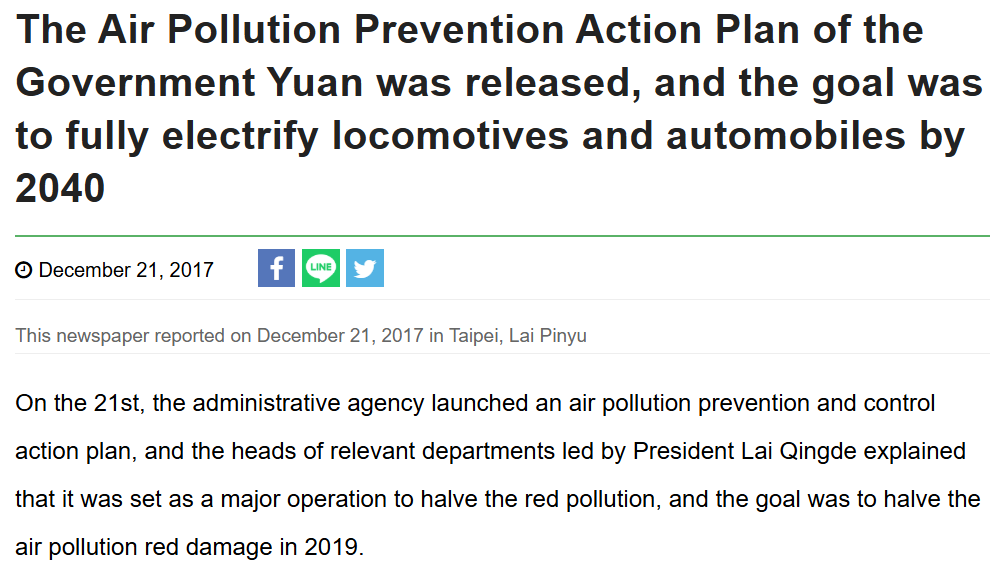
\includegraphics[height=3in]{notes/media/air_quality_reform_news.png}\\
    \textit{Вирізка зі статті про початок реформи}
\end{center}

Індекс забруднення повітря базується на рівні 6 атмосферних забруднювальних речовин, зокрема діоксиду сірки ($SO_2$), діоксиду азоту ($NO_2$), твердих частинок ($PM_{10}$), твердих частинок ($PM_{2.5}$), окису вуглецю ($CO$) і озону ($O_3$). 
\textit{Particulate matter} (PM) це мікроскопічні тверді частинки. Фактично - це все в повітрі, що не є газом, і складається з величезного різноманіття хімічних сполук та матеріалів, деякі з яких можуть бути токсичними. 
Частинки мають діаметр менше 10 мкм (PM10) і діаметр менше 2.5 мкм (PM2.5).
\subsection{Постановка задачі}
З огляду на мету та досліджувану галузь, було поставлено такі питання: 

\begin{enumerate}
    \item Чи впливає швидкість вітру (windspeed) на концентрацію частинок PM2.5 і PM10?
    \item Чи існує кореляція між рівнем забруднення повітря (AQI) і типом головного забруднювача (pollutant) в різних районах?
    \item Як зміни в концентрації озону (O3) впливають на загальний рівень забруднення повітря (AQI)?
    \item Які регіони (county) мають найвищий середній рівень забруднення повітря (AQI) протягом року?
    \item Як змінюється якість повітря (status) протягом доби в різних районах?
    \item Як змінюється концентрація PM2.5 і PM10 в залежності від швидкості вітру (windspeed) і напрямку вітру (winddirec) в різних регіонах?
    \item Як змінився загальний рівень забруднення по регіонам після початку реформи? 
    \item Чи існує залежність між початком реформ та показниками забруднення? 
    \item Як змінюється якість повітря залежно від станції виміру у містах?
\end{enumerate}

    
\newpage
\section{ОСНОВНА ЧАСТИНА}
\subsection{Опис даних}
Так як реформа досі продовжується, то дані оновлюються в живому часі. Тому для дослідження було взято результати \textit{з 25 листопада 2016 по 31 серпня 2024}
\footnote{\href{https://data.moenv.gov.tw/en/dataset/detail/aqx_p_488}{Покликання на офіційний датасет Міністерства довкілля Тайваню}}

Відповідно до базового розвідкованого аналізу, було отримано наступні характеристики набору даних: 

\begin{itemize}
    \item Кількість рядків: 5\,882\,208
    \item Кількість стовпців: 22
    \item Початковий опис даних: 
    \begin{table}[h!]
\centering
\begin{tabular}{|>{\raggedright\arraybackslash}p{3cm}|p{5cm}|p{3cm}|}
\hline
\textbf{Column} & \textbf{Description} & \textbf{Data Type} \\
\hline
date & Date and time of the reading & Text \\
\hline
sitename & Station name & Text \\
\hline
county & County or city & Text \\
\hline
aqi & Air Quality Index & Numeric \\
\hline
pollutant & Main pollutant & Text \\
\hline
status & Status of air quality & Text \\
\hline
so2 & Sulfur Dioxide in ppb & Numeric \\
\hline
co & Carbon Monoxide in ppm & Numeric \\
\hline
o3 & Ozone in ppb & Numeric \\
\hline
o3\_8hr & 8-hour average of Ozone & Numeric \\
\hline
pm10 & Particulate matter under 10m & Numeric \\
\hline
pm2.5 & Particulate matter under 2.5m & Numeric \\
\hline
no2 & Nitrogen Dioxide in ppb & Numeric \\
\hline
nox & Nitrogen Oxides in ppb & Numeric \\
\hline
no & Nitric Oxide in ppb & Numeric \\
\hline
windspeed & Wind speed in m/sec & Numeric \\
\hline
winddirec & Wind direction in degrees & Numeric \\
\hline
unit & Unit of measurement & Text \\
\hline
co\_8hr & 8-hour average of CO & Numeric \\
\hline
pm2.5\_avg & Moving average of PM2.5 & Numeric \\
\hline
pm10\_avg & Moving average of PM10 & Numeric \\
\hline
so2\_avg & Moving average of SO2 & Numeric \\
\hline
longitude & Longitude of the site & Numeric \\
\hline
latitude & Latitude of the site & Numeric \\
\hline
siteid & Station ID & Numeric \\
\hline
\end{tabular}
\label{tab:data_columns}
\end{table}
\end{itemize}

\subsection{Підготовка даних}
Для того, щоб розпочати розвідковий аналіз, було проведено очищення та попередня підготовка даних, а саме: 
\begin{itemize}
    \item Перший огляд датасету показав, що деякі числові стовпці зчитались як текстові. 
    Щоб виправити це, було застосовано функцію `problems` показало, що:
        \begin{itemize}
            \item іноді замість порожнього значення використовується $-$ або ND. Через це відповідні колонки стають текстовими
            \item трапляється неправильний формат дати (роздільник $/$ замість очікуваного $-$).
        \end{itemize}
   \textbf{Рішення:} До функції $read\_csv$ додано аргумент $na$, який вказує, що значення $" \ "$, $"\ -"$ і $"ND"$ треба сприймати як порожні. Виправлено формат дати.
   
   Колонки $'sitename'$, $'county'$, $'pollutant'$ і $'status'$ перетворено на категорійні. Проблеми із типами даних на цьому вирішено.
   
   \newpage
   
    \item Під час перевірки закодаваних і неадекватних даних у кожному стовпці було отримано наступні результати: 
         \begin{itemize}
             \item Стовпці, що містять очевидно кодові значення:
             \begin{itemize}
                \item \textbf{aqi} - кодові: -1
                
                Рядки, де $\text{aqi} = -1$, майже повністю заповнені NA. Такі рядки займають близько $0.2\%$
                \item \textbf{so2, co, o3, pm10, pm2.5}  - кодові: -999
                
                Є підозрілі від'ємні числа. Можна припустити, що від'ємні показники є наслідком неідеалньості калібрування датчиків (тобто вони є справжніми, а не кодовими). Також у датасеті зафіксовані значно більші за модулем додатні концентрації, тому зсув показників є незначним.
                \item \textbf{winddirec} - кодові: 990
             \end{itemize}
             
            \textbf{ Рішення:} Кодові значення замінимо на NA.

             \item Стовпці, що містять від'ємні значення:
             \begin{itemize}
                \item \textbf{so2, co, no2,  o3, nox, no, windspeed, co\_8hr, pm2.5\_avg, pm10\_avg , so2\_avg} 
                \item \textbf{o3\_8hr} - кодові: -1

                Є від'ємне число -1. Хоча воно і схоже на кодове, за аналогією до попередніх колонок, припустимо, що воно справжнє. До того ж, частка таких рядків дуже мала: у цьому можна переконатися, поглянувши на гістограму.
             \end{itemize}

             \textbf{Рішення:} Припуститимо, що від'ємні показники є справжніми, а не кодовими, і виникли через незначний зсув у калібруванні датчиків. За неохідності (наприклад, для логаритмування) цей зсув можна буде компенсувати додаванням певного числа до всіх значень відповідної колонки.
             
             \item Стовпці, які можна видалити, користь під сумнівом:
             \begin{itemize}
                 \item \textbf{unit} - порожня колонка
                 \item \textbf{longitude, latitude, siteid}  - корисність під сумнівом
             \end{itemize}
             
             \textbf{Рішення:} Видалимо непотрібні стовпці.
         \end{itemize}
    
    \item Було перевірено та проаналізовано кількість пропущених значень у кожному рядку та стовпці. Відповідно, стовпці в яких було відсутньо більше третини значень, було вирішено видалити, а саме в стовпці "pollutant" було відсутньо більше 5%.
    
    \textbf{Рішення:} видалити стовпець.
    
    \item Стовпці в яких було відмічено не значний відсоток пропущених даних,попередньо було залишено без змін. 
    
    Можливе рішення на майбутнє: заповнити або середніми значеннями (для числового типу), або часто повторюваними (для категоріального та текстового) 
    
    \item Було додано додатковий стовпчик з бінарним типом даних: 1 - після реформи, 0 - до реформи. Це дозволить проаналізувати та порівняти вплив реформи на якість повітря.
\end{itemize}


В результаті після "очистки" даних, отримали такі основні характеристики:
 \begin{enumerate}      
    \item Розмір набору даних: 
        \begin{itemize}
            \item Кількість рядків: 5\,882\,208
            \item Кількість стовпців: 16
        \end{itemize} 
    \item Кількість змінних:
        \begin{itemize}
            \item Факторні (factor)  - 3
            \item Логічні (logical) -  1
            \item Числові (numeric) -  11
            \item Тип дати (POSIXct) -  1 
        \end{itemize} 

    \pagebreak
    \item Кількість пропущених даних:
    
    \begin{table}[h!]
    \centering
\begin{tabular}{llccc}

\toprule
\textbf{Variable Type} & \textbf{Variable} & \textbf{Missing} & \textbf{Complete rate} \\
\midrule
Factor   & sitename      & 0      & 1     \\
         & county        & 0      & 1     \\
         & status        & 142718 & 0.976 \\
Logical  & after\_reform & 0      & 1     \\
Numeric  & aqi           & 50411  & 0.991 \\
         & so2           & 139794 & 0.976 \\
         & co            & 154139 & 0.974 \\
         & o3            & 207427 & 0.965 \\
         & pm10          & 146655 & 0.975 \\
         & pm2.5         & 202228 & 0.966 \\
         & no2           & 166000 & 0.972 \\
         & nox           & 169147 & 0.971 \\
         & no            & 169478 & 0.971 \\
         & windspeed     & 302683 & 0.949 \\
         & winddirec     & 303499 & 0.948 \\
POSIXct  & date          & 0      & 1     \\
\bottomrule
\end{tabular}
\caption{Missing data statistics}
\label{tab:summary}
\end{table}

    \begin{center}
        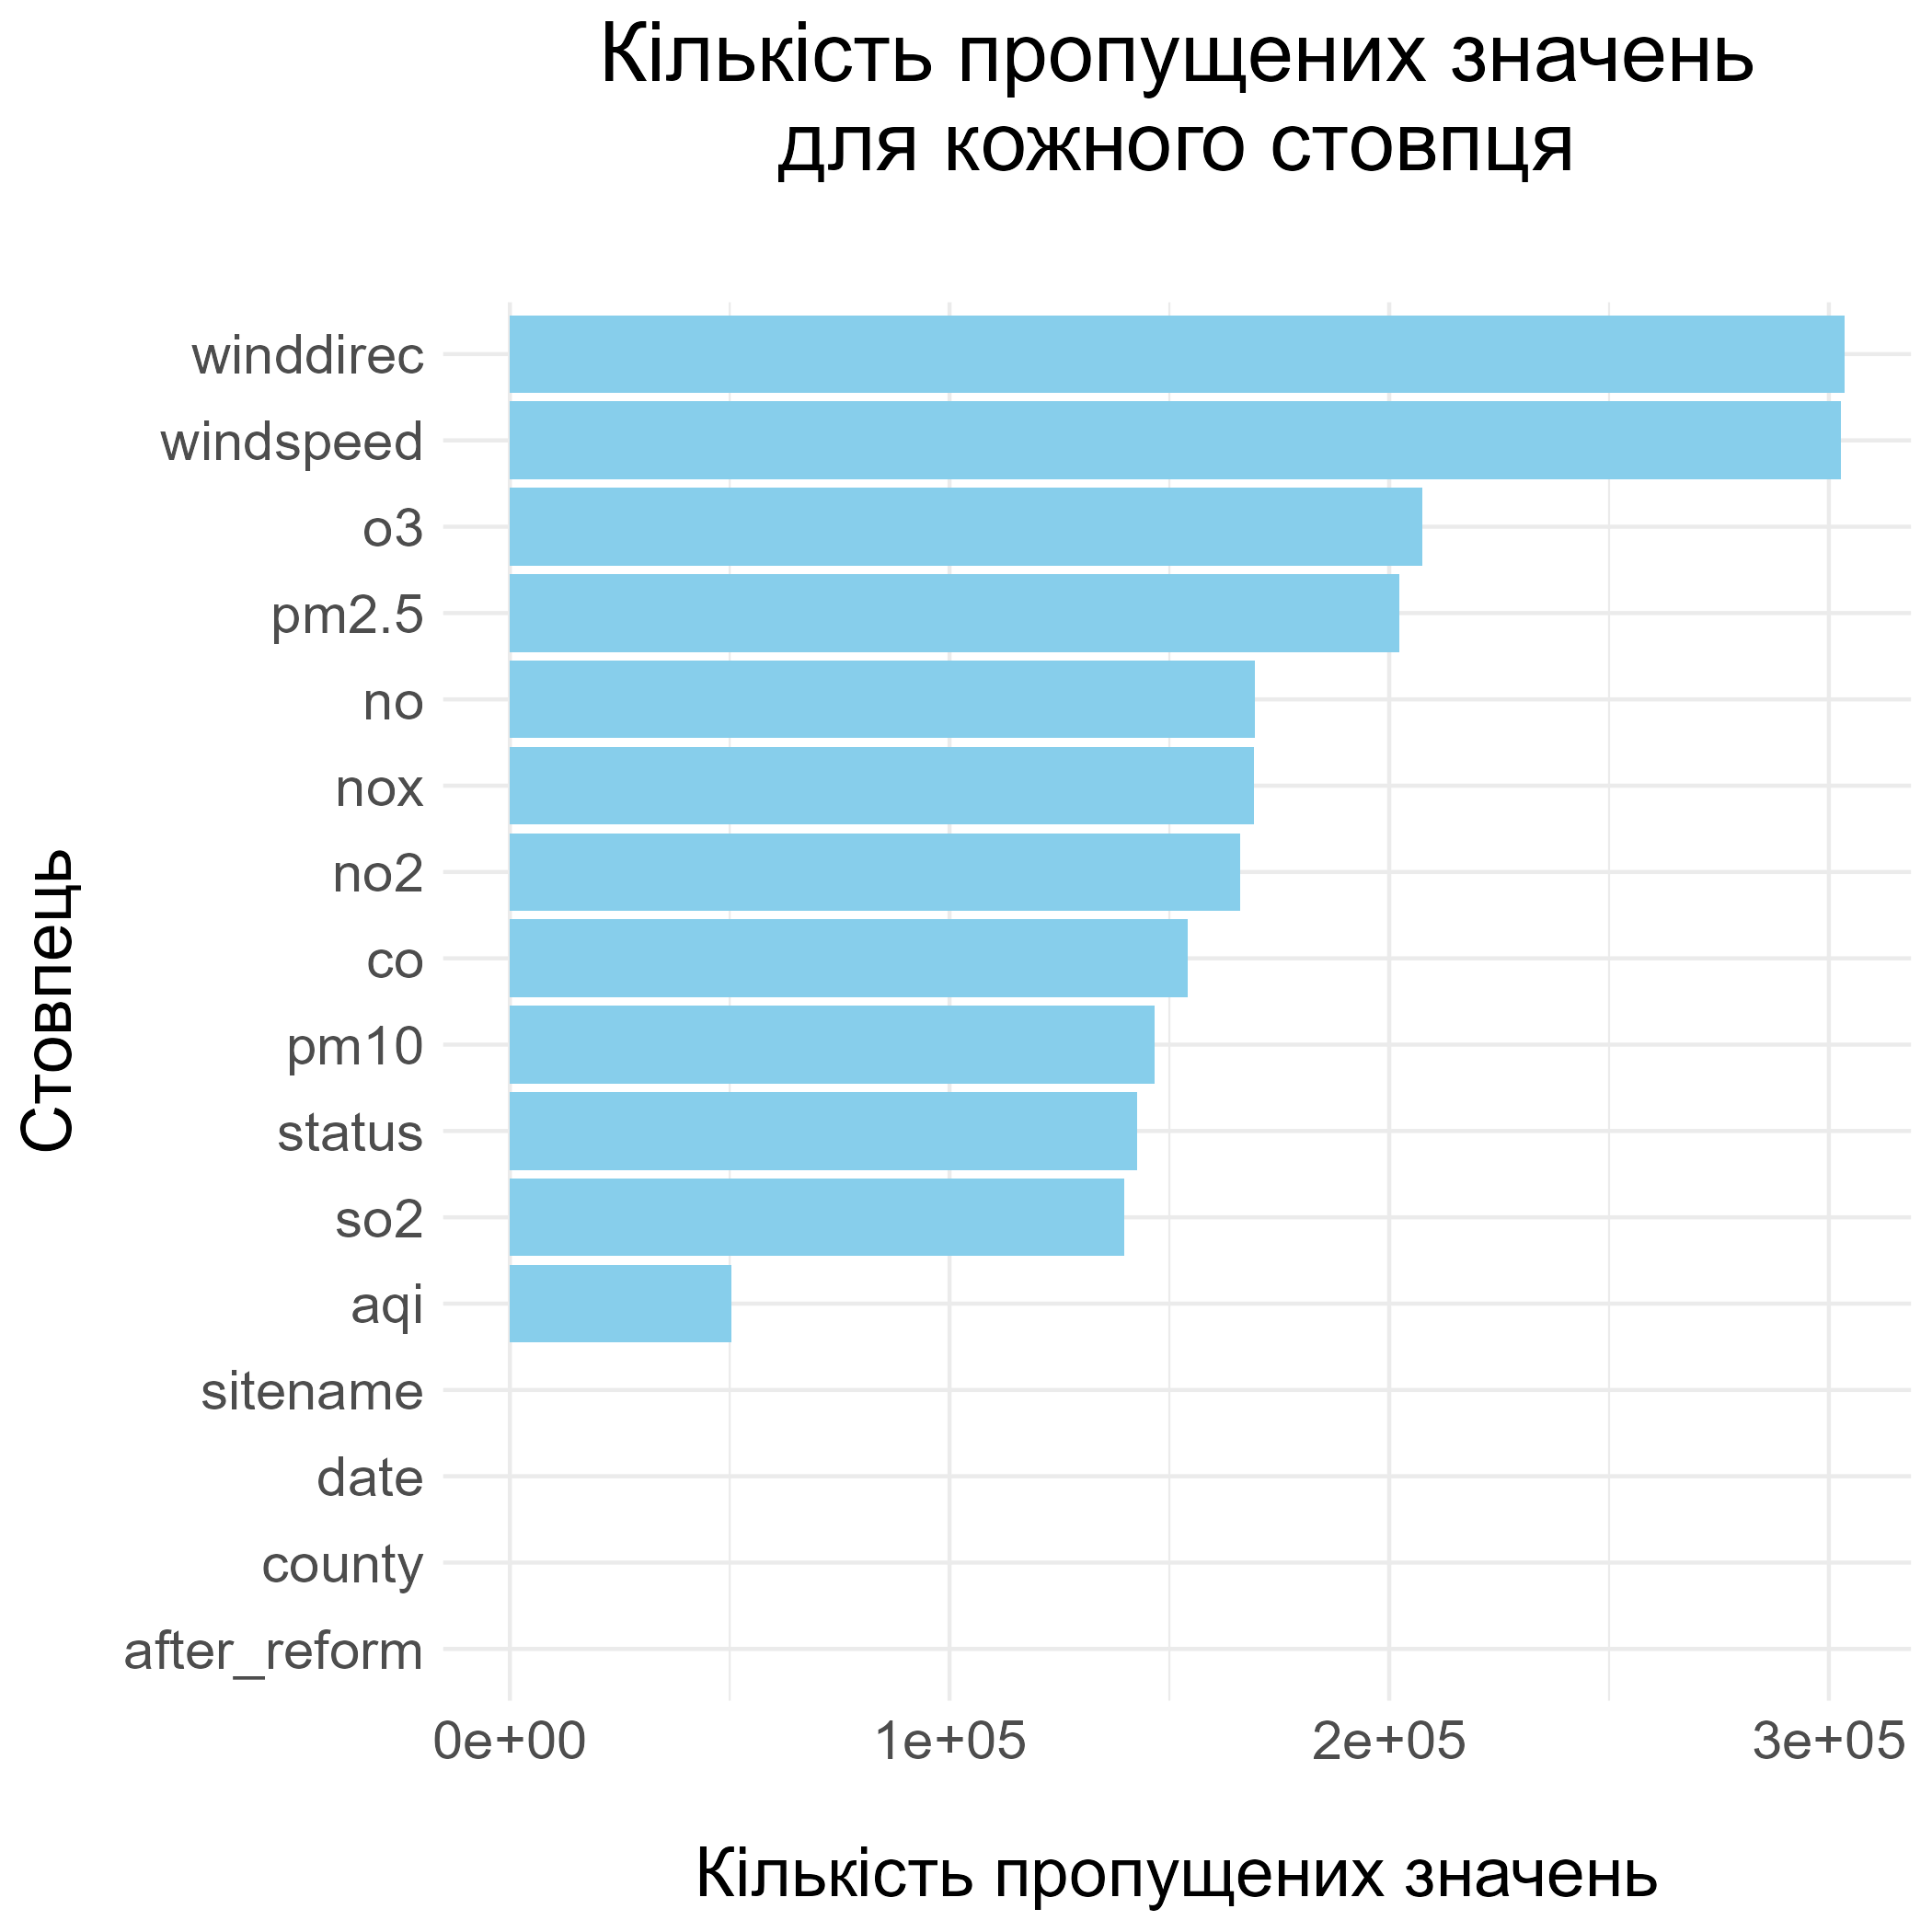
\includegraphics[height=4.5in]{plots/missed_data.png}
    \end{center}
    
    \pagebreak
    
    \item Дескриптивнi статистики:

    \begin{itemize}
        \item Числові змінні:

\begin{tabular}{lcccccc}
\toprule
\textbf{Variable} & \textbf{Min.} & \textbf{1st Qu.} & \textbf{Median} & \textbf{Mean} & \textbf{3rd Qu.} & \textbf{Max.} \\
aqi       & 0      & 32   & 47    & 54.26 & 70   & 500    \\
so2       & -4.1   & 1    & 1.7   & 1.99  & 2.5  & 255.4  \\
co        & -0.27  & 0.19 & 0.29  & 0.34  & 0.41 & 38.58  \\
o3        & -1     & 16   & 28.3  & 30.42 & 42   & 410    \\
pm10      & 0      & 18   & 28    & 34.38 & 45   & 1407   \\
pm2.5     & 0      & 8    & 14    & 16.85 & 23   & 1000   \\
no2       & -27.78 & 5    & 9     & 11.25 & 15   & 351.05 \\
nox       & -1.6   & 6.2  & 10.8  & 14.72 & 18   & 431    \\
no        & -7.2   & 0.7  & 1.4   & 3.45  & 2.7  & 391.31 \\
windspeed & -0.4   & 1.1  & 1.8   & 2.21  & 2.9  & 41     \\
winddirec & 0      & 55   & 150   & 163.3 & 270  & 359    \\
\midrule
\end{tabular}

    \item Факторні змінні:
    
\begin{tabular}{ccccc}
\toprule
\textbf{Variable} & \multicolumn{4}{c}{\textbf{Count}} \\
status & Good    & Moderate & \vtop{\hbox{\strut Unhealthy for}\hbox{\strut Sensitive Groups}} & Unhealthy \\
       & 3185191 & 2159158  & 343909  & 51008     \\
       & Very Unhealthy  & Hazardous         &                  & \\
       & 173             & 51                &                  & \\
county & Changhua County & Chiayi City       & Chiayi County    & Hsinchu City  \\
       & 293423          & 71912             & 143986           & 75850         \\
       & Hsinchu County  & Hualien County    & Kaohsiung City   & Keelung City  \\
       & 143846          & 71912             & 888497           & 71913         \\
       & Kinmen County   & Lienchiang County & Miaoli County    & Nantou County \\
       & 71913           & 71914             & 219683           & 216420        \\
       & New Taipei City & Penghu County     & Pingtung County  & Taichung City \\
       & 898819          & 71910             & 305495           & 367033        \\
       & Tainan City     & Taipei City       & Taitung County   & Taoyuan City  \\
       & 366827          & 503766            & 143809           & 448718        \\
       & Yilan County    & Yunlin County     &                  &               \\
       & 147071          & 287491            &                  &               \\
\end{tabular}
    
    \item Дата:
    
\begin{tabular}{ccc}
\toprule
\textbf{Variable} & \textbf{Min.} & \textbf{Max.} \\
\midrule
date & 2016-11-25 & 2024-08-31 \\
     & 13:00:00   & 23:00:00   \\
\midrule
\end{tabular}

     \item Логічні:
     
\begin{tabular}{ccc}
\textbf{Variable} & \textbf{True} & \textbf{False} \\
after\_reform     &  654783       &  5227425       \\               
\end{tabular}    
    
    \end{itemize}
    
    \pagebreak

    \item Зменшення набору даних:

    На більшість питань розвідкового аналізу можна дати відповідь не маючи весь набір
    даних. Було прийнято рішення зменшити набір даних, тобто вибрати тільки рядки, 
    починаючи з певного року.

    Знайдемо кількість рядків в кожному році:

    \begin{tabular}{cc}
        \textbf{Year} & \textbf{Count} \\
        2016          & 65431          \\
        2017          & 664415         \\
        2018          & 671559         \\
        2019          & 712824         \\
        2020          & 716022         \\
        2021          & 1070296        \\
        2022          & 748667         \\
        2023          & 736902         \\
        2024          & 496092         \\
    \end{tabular}

    Знайдемо кумулятивну суму з кінця, щоб визначити кількість даних, яка буде вибрана 
    починаючи з відповідного року:

    \begin{tabular}{cc}
        \textbf{Year} & \textbf{Accumulated count} \\
        2016 & 5882208 \\
        2017 & 5816777 \\
        2018 & 5152362 \\
        2019 & 4480803 \\
        2020 & 3767979 \\
        2021 & 3051957 \\
        2022 & 1981661 \\
        2023 & 1232994 \\
        2024 & 496092  \\
    \end{tabular}

    Було прийнято рішення вибрати набір даних починаючи з 2023 року 
    (1\,232\,994 з 5\,882\,208 рядків).

    Надалі будемо зазначати на якому наборі даних був виконаний аналіз. Зменшений
    датасет назвемо \textit{trimmed}.
    
    \item Викиди:

    \quad \textit{Був використаний trimmed набір даних}
    
    Для пошуку викидів використаємо \textit{фільтр Гампеля}:

    \begin{displayquote}
    Викидом є будь‑яке спостереження 
    $x \notin [M - 3 \cdot \text{MAD}; M + 3 \cdot \text{MAD}]$, 
    
    де $\text{MAD} = \dfrac{1}{\Phi^{-1}(0.75)} \cdot \text{median}(\pmb{x} - M)$,
    $M = \text{median}(\pmb{x})$
    \end{displayquote}

    Кількість викидів по кожній змінній:

    \begin{tabular}{ccc}
    \textbf{Variable} & \textbf{Count} & \textbf{Relative count} \\
    aqi        & 26759  & 0.0217  \\
    so2        & 57595  & 0.0467  \\
    co         & 53340  & 0.0433  \\
    o3         & 5154   & 0.00418 \\
    pm10       & 43393  & 0.0352  \\
    pm2.5      & 43913  & 0.0356  \\
    no2        & 58132  & 0.0471  \\
    nox        & 82640  & 0.067   \\
    no         & 159513 & 0.129   \\
    windspeed  & 43491  & 0.0353 \\
    winddirec  & 0      & 0       \\
    \end{tabular}

   \pagebreak
    
    Гістограма кількості викидів:

    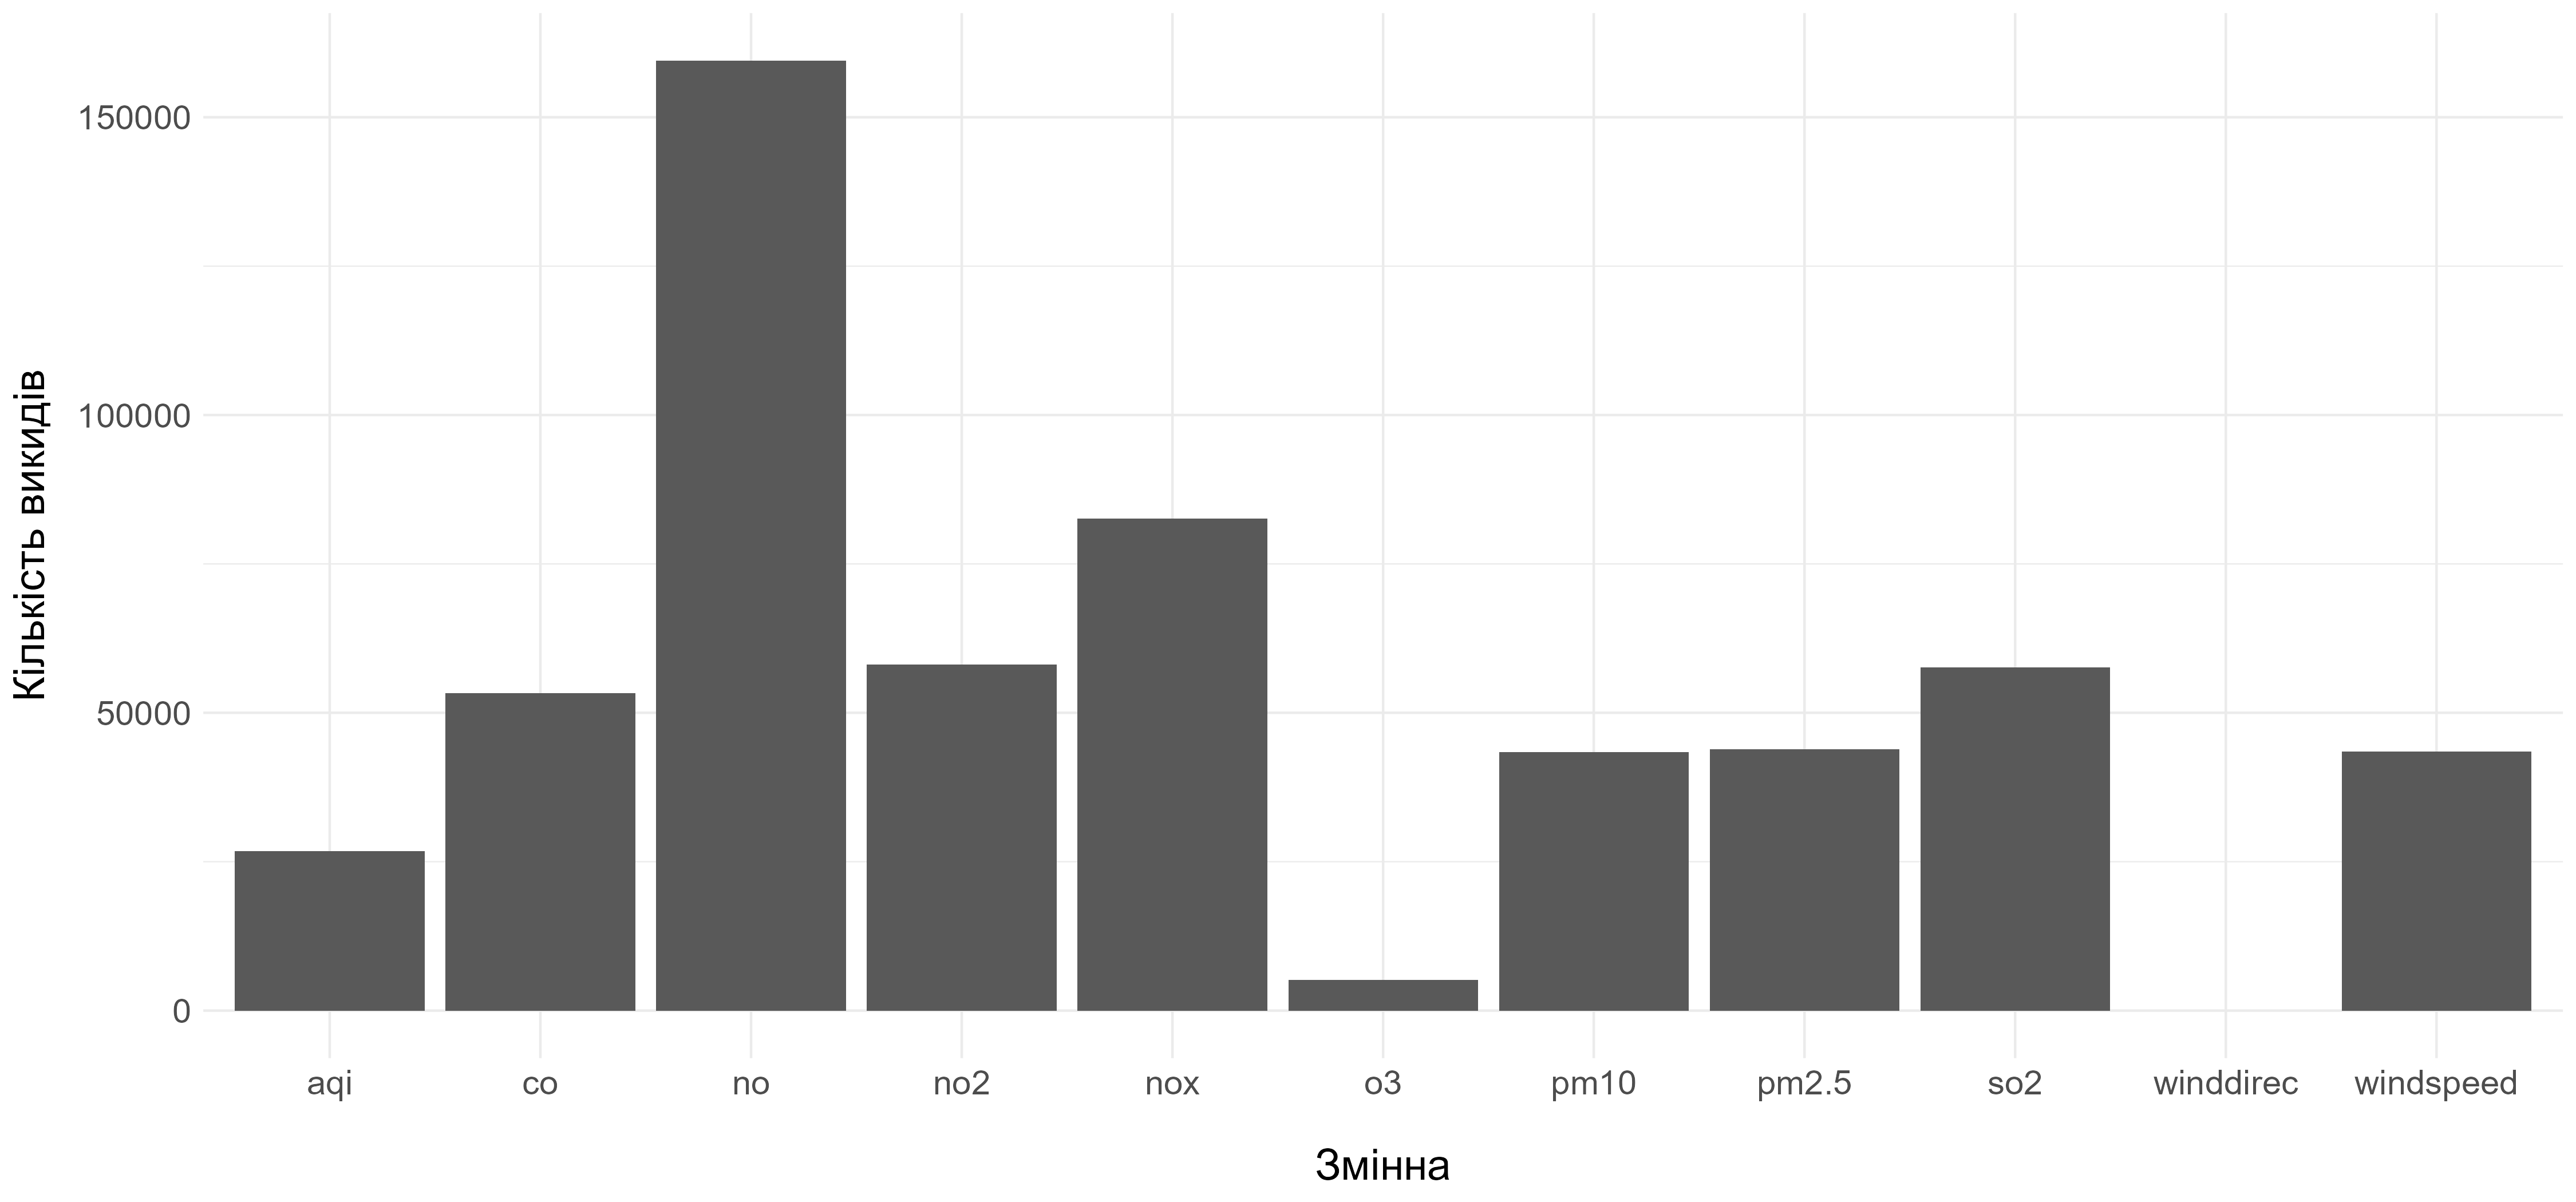
\includegraphics[height=2.7in]{plots/outliers/count-bar.png}
    
    Гістограма кількості викидів залежно від регіону:

    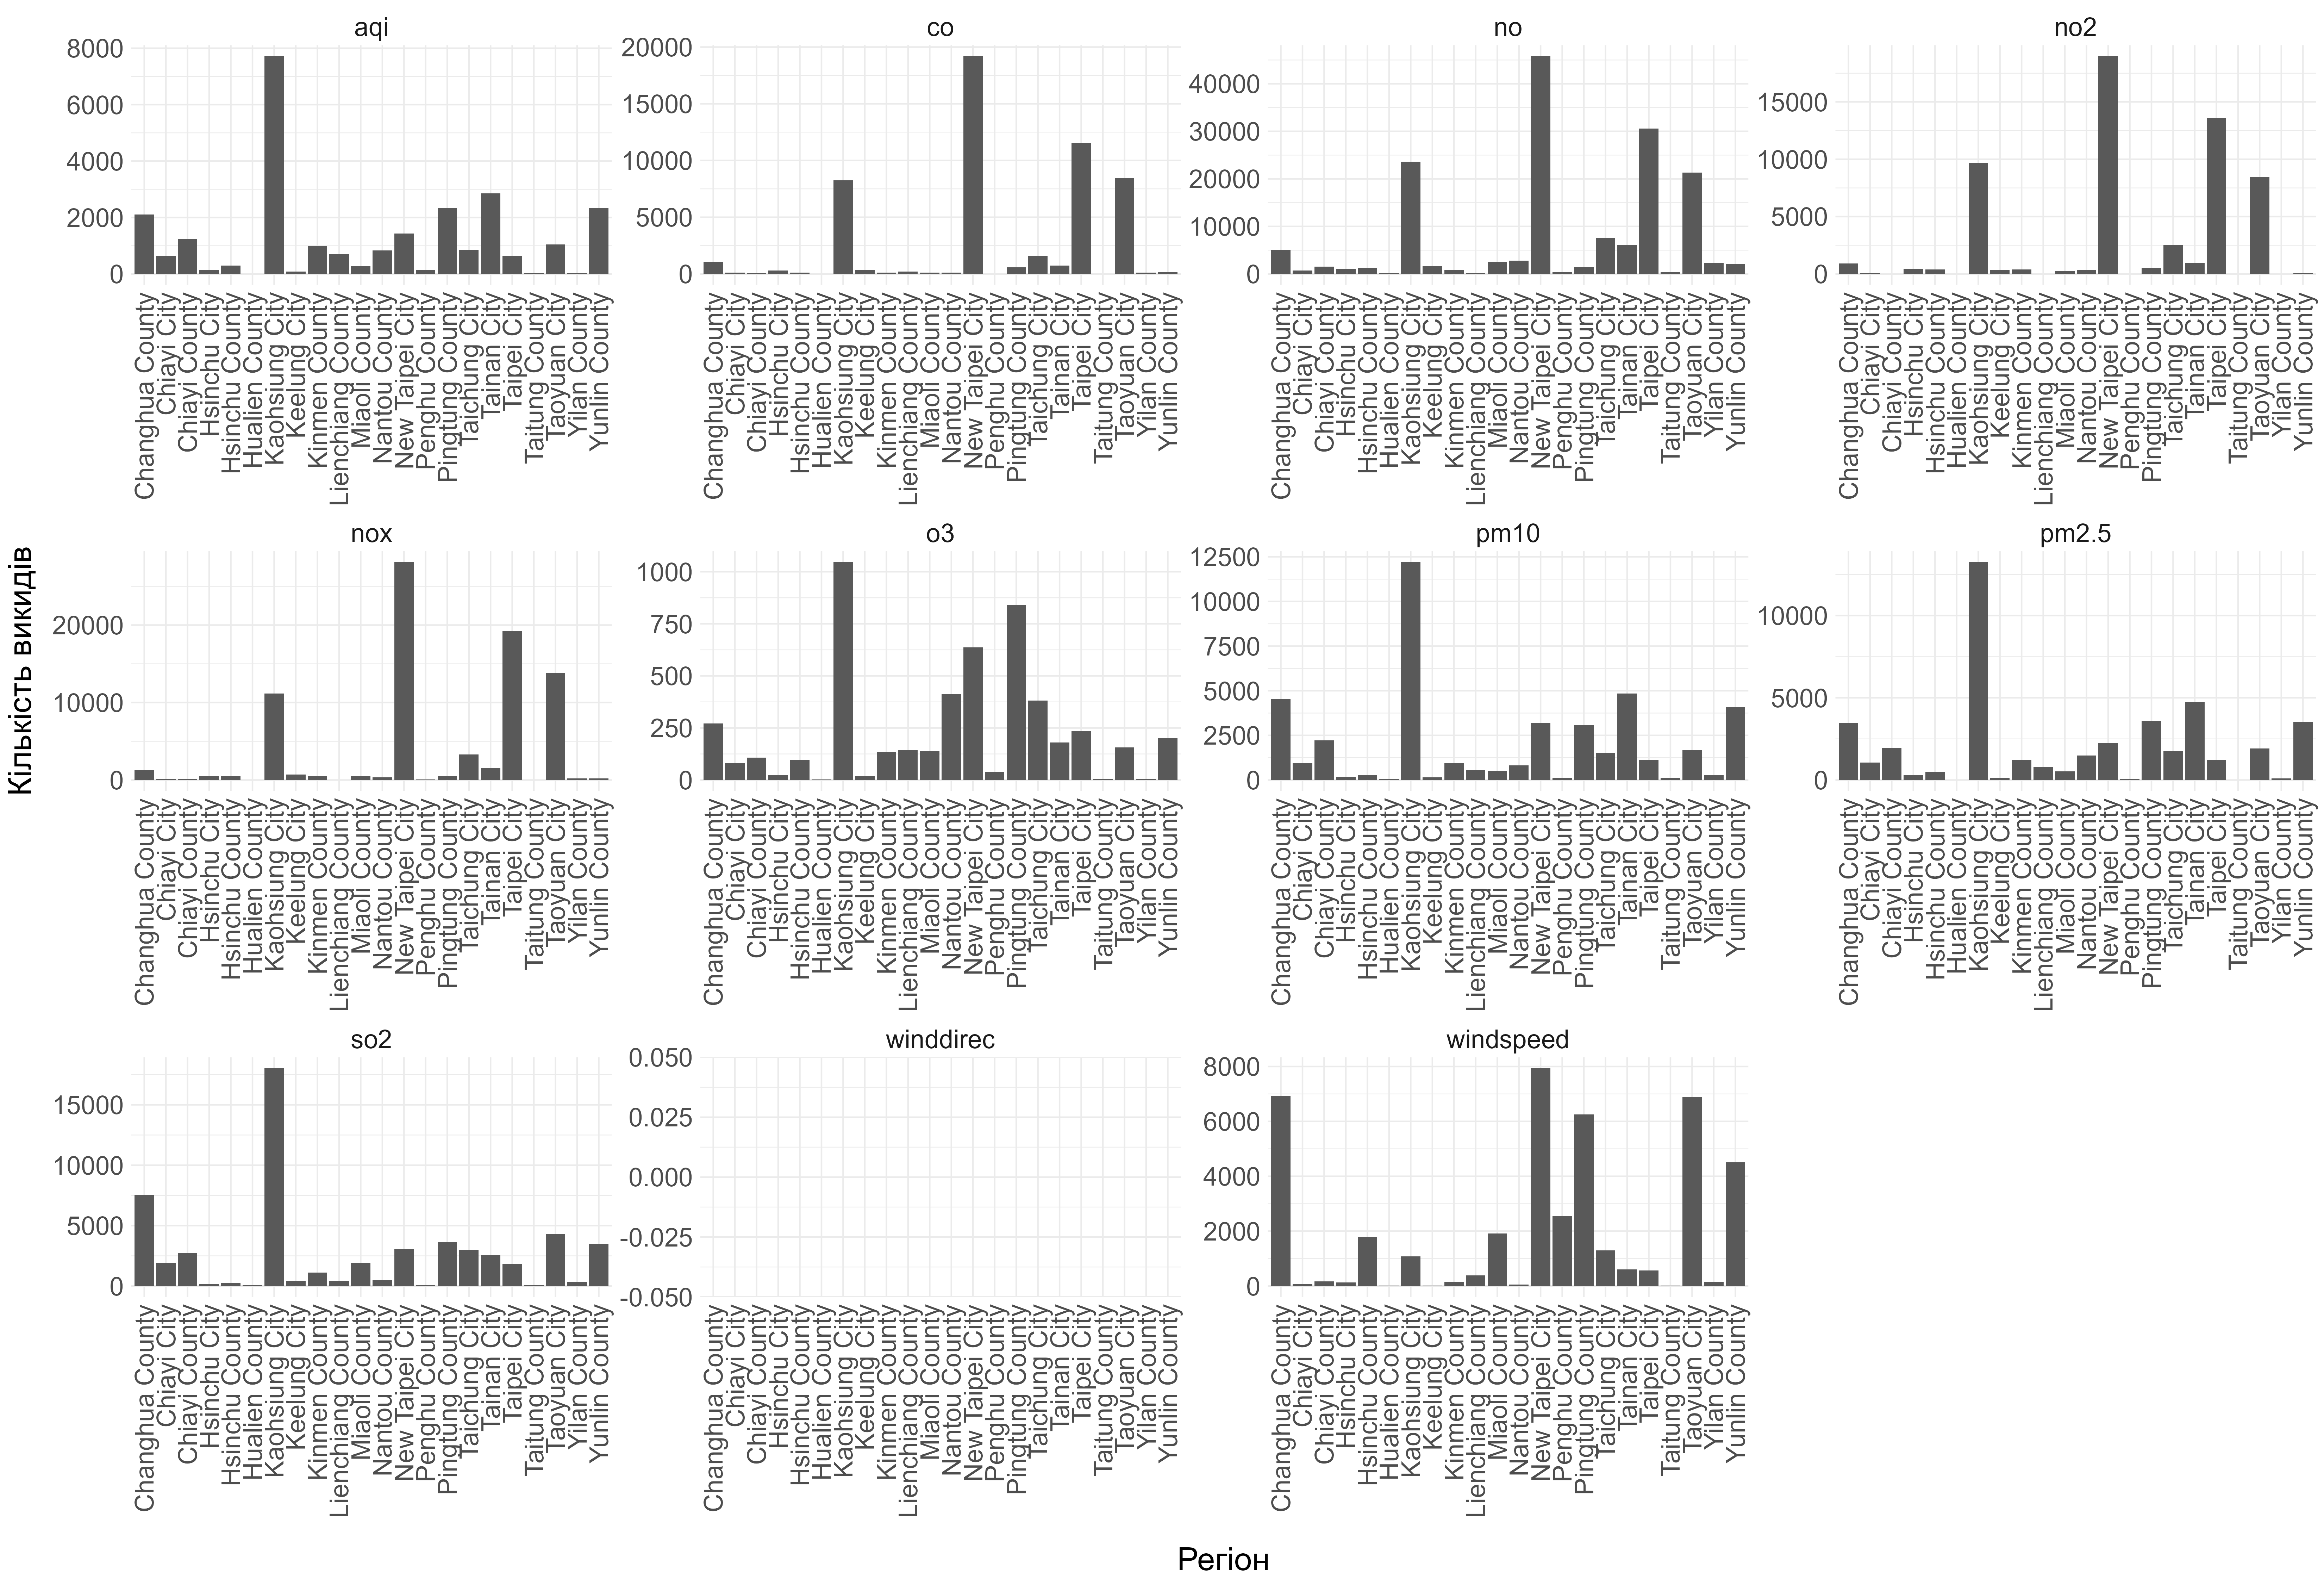
\includegraphics[width=6in]{plots/outliers/count-bar-county.png}

    На гістограмі можна замітити, що кількість викидів не розподілена рівномірно
    по регіонам.

    \pagebreak

    Гістограма розсіювання:

    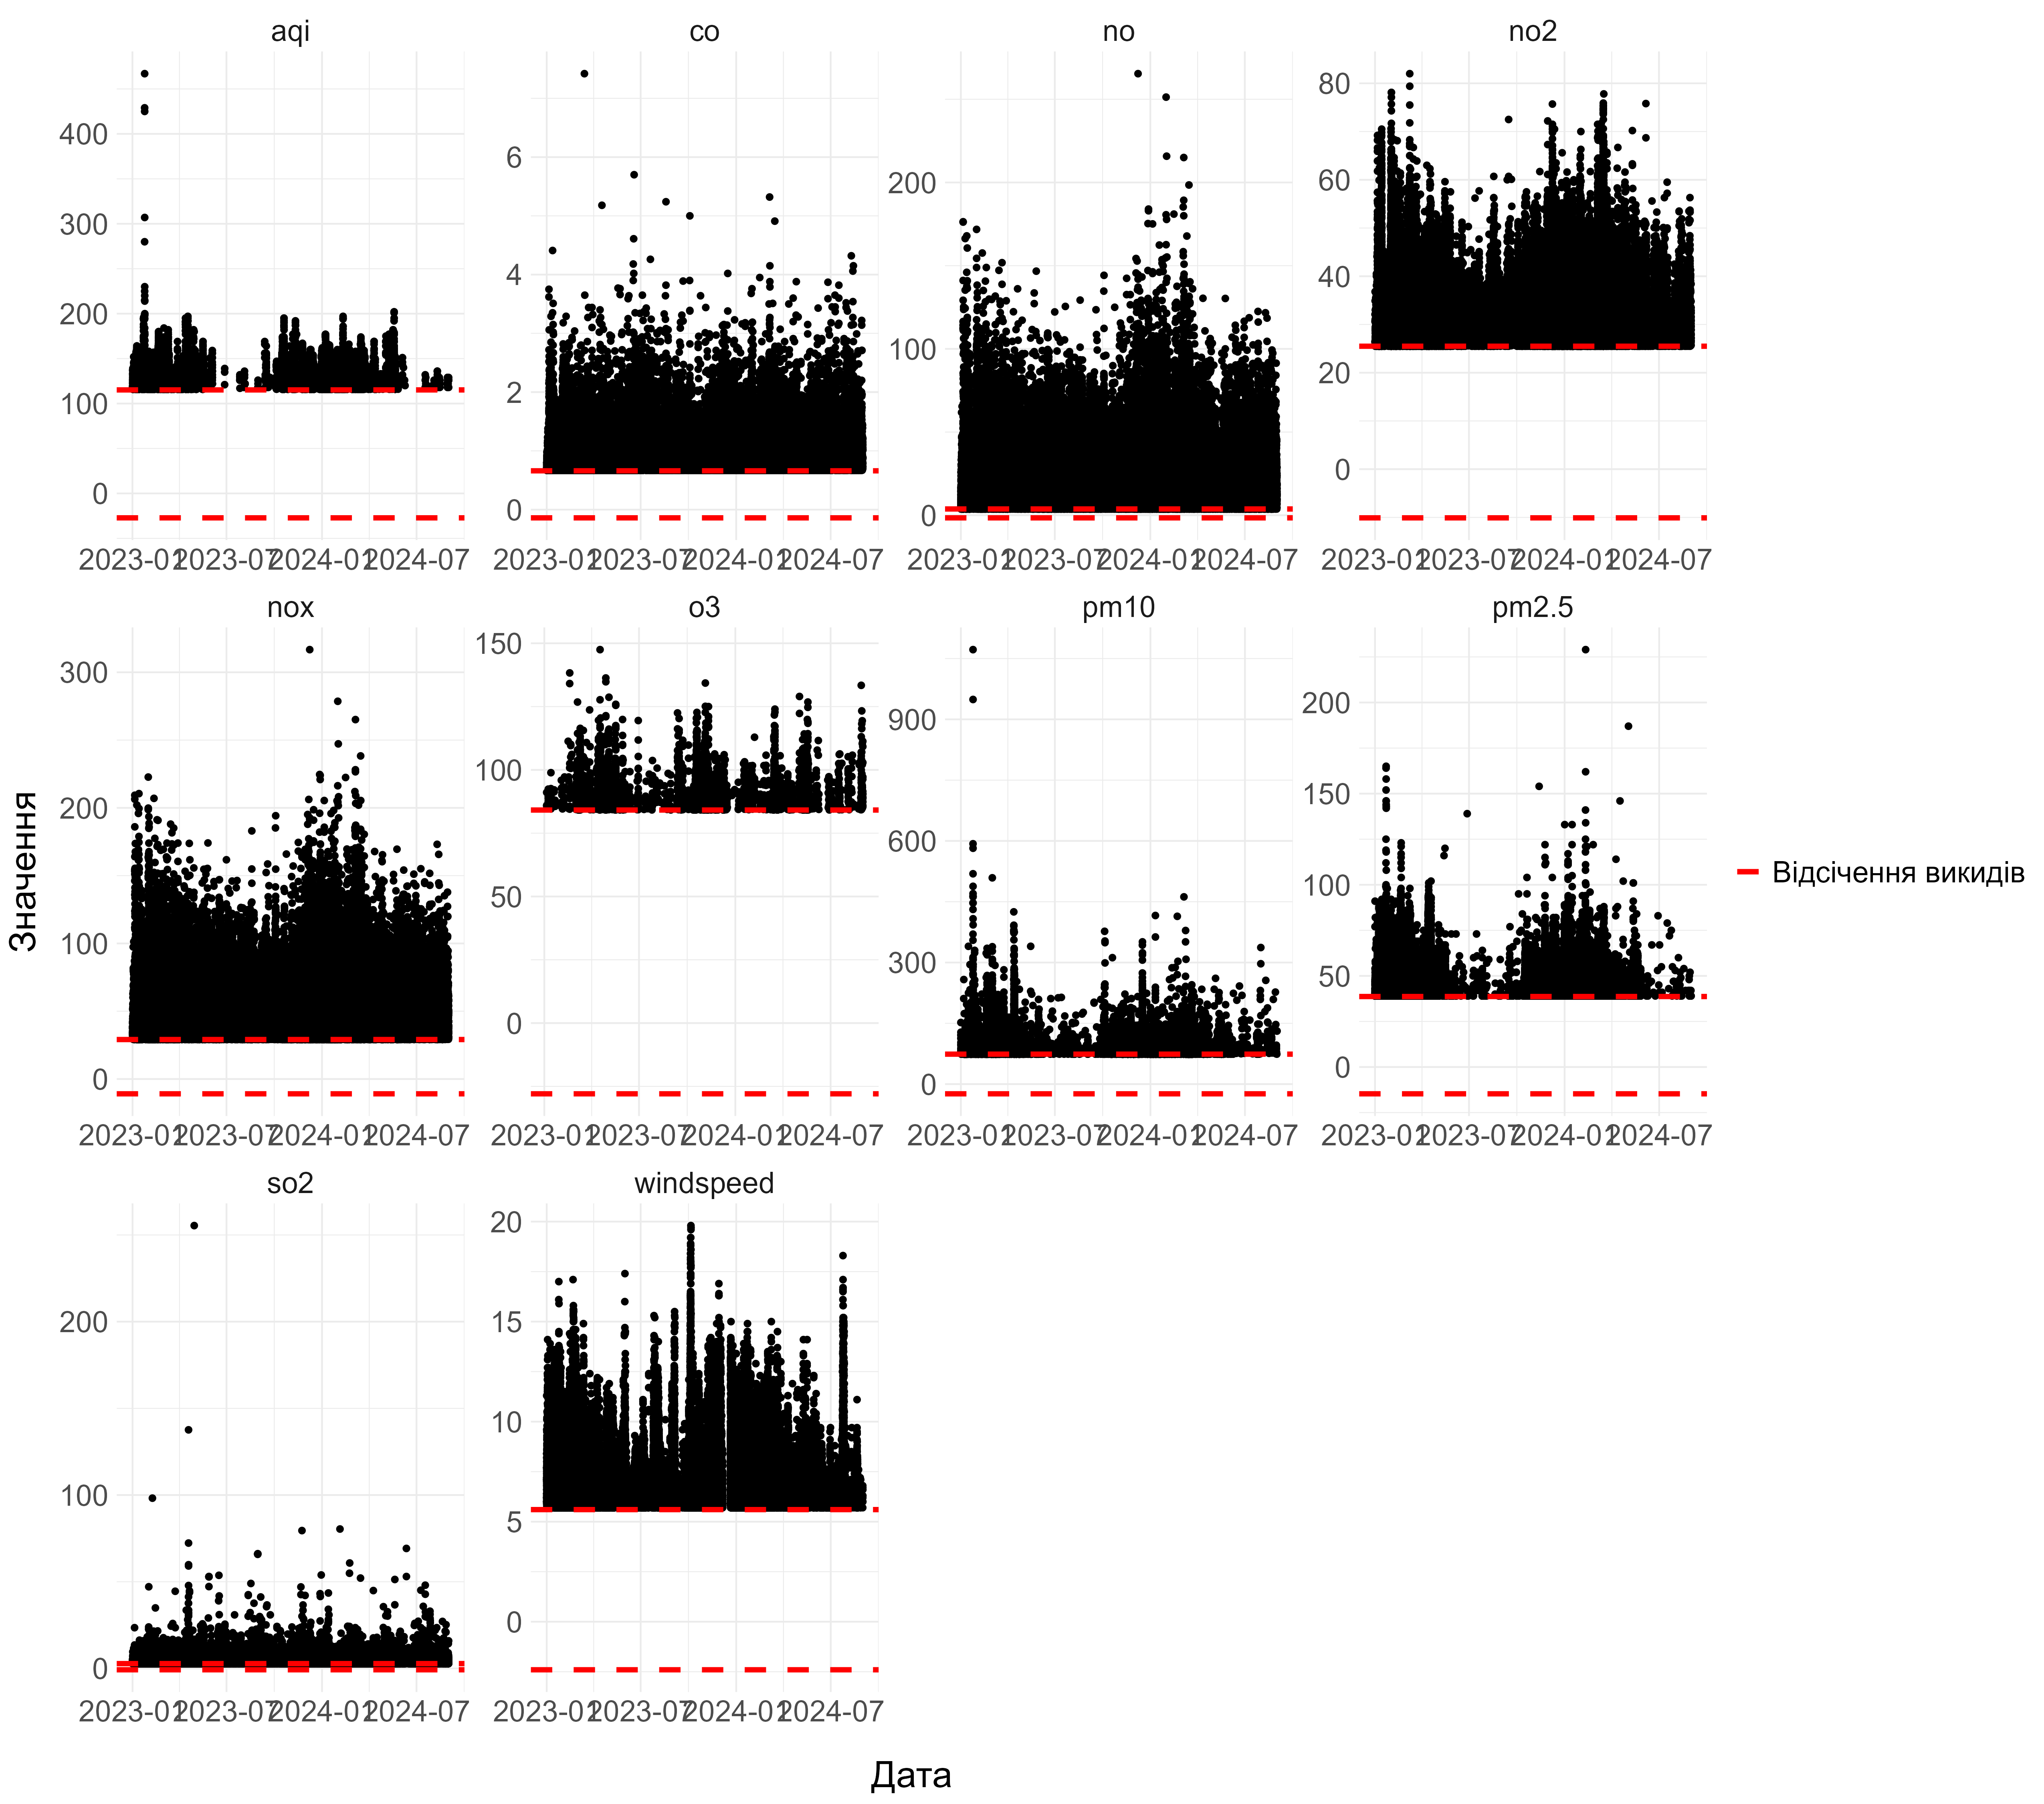
\includegraphics[width=6in]{plots/outliers/scatter.png}

    Червоними лініями позначені проміжки, в яких значення змінної не класифікується
    як викид. На діаграмі розсіювання можна замітити значення, які набагато більші за
    інші викиди. Можна припустити, що вони є помилками датчиків, які вимірювали якість
    повітря.

    Було прийнято рішення не змінювати значення, або видаляти викиди. Натомість будемо
    використовувати міри вибірок, які більш стійкі до викидів. 

    \pagebreak

    \item Розподіли змінних

    Для побудови QQ-графіків, випадковим чином виберемо з датасету 10\,000 рядків.

    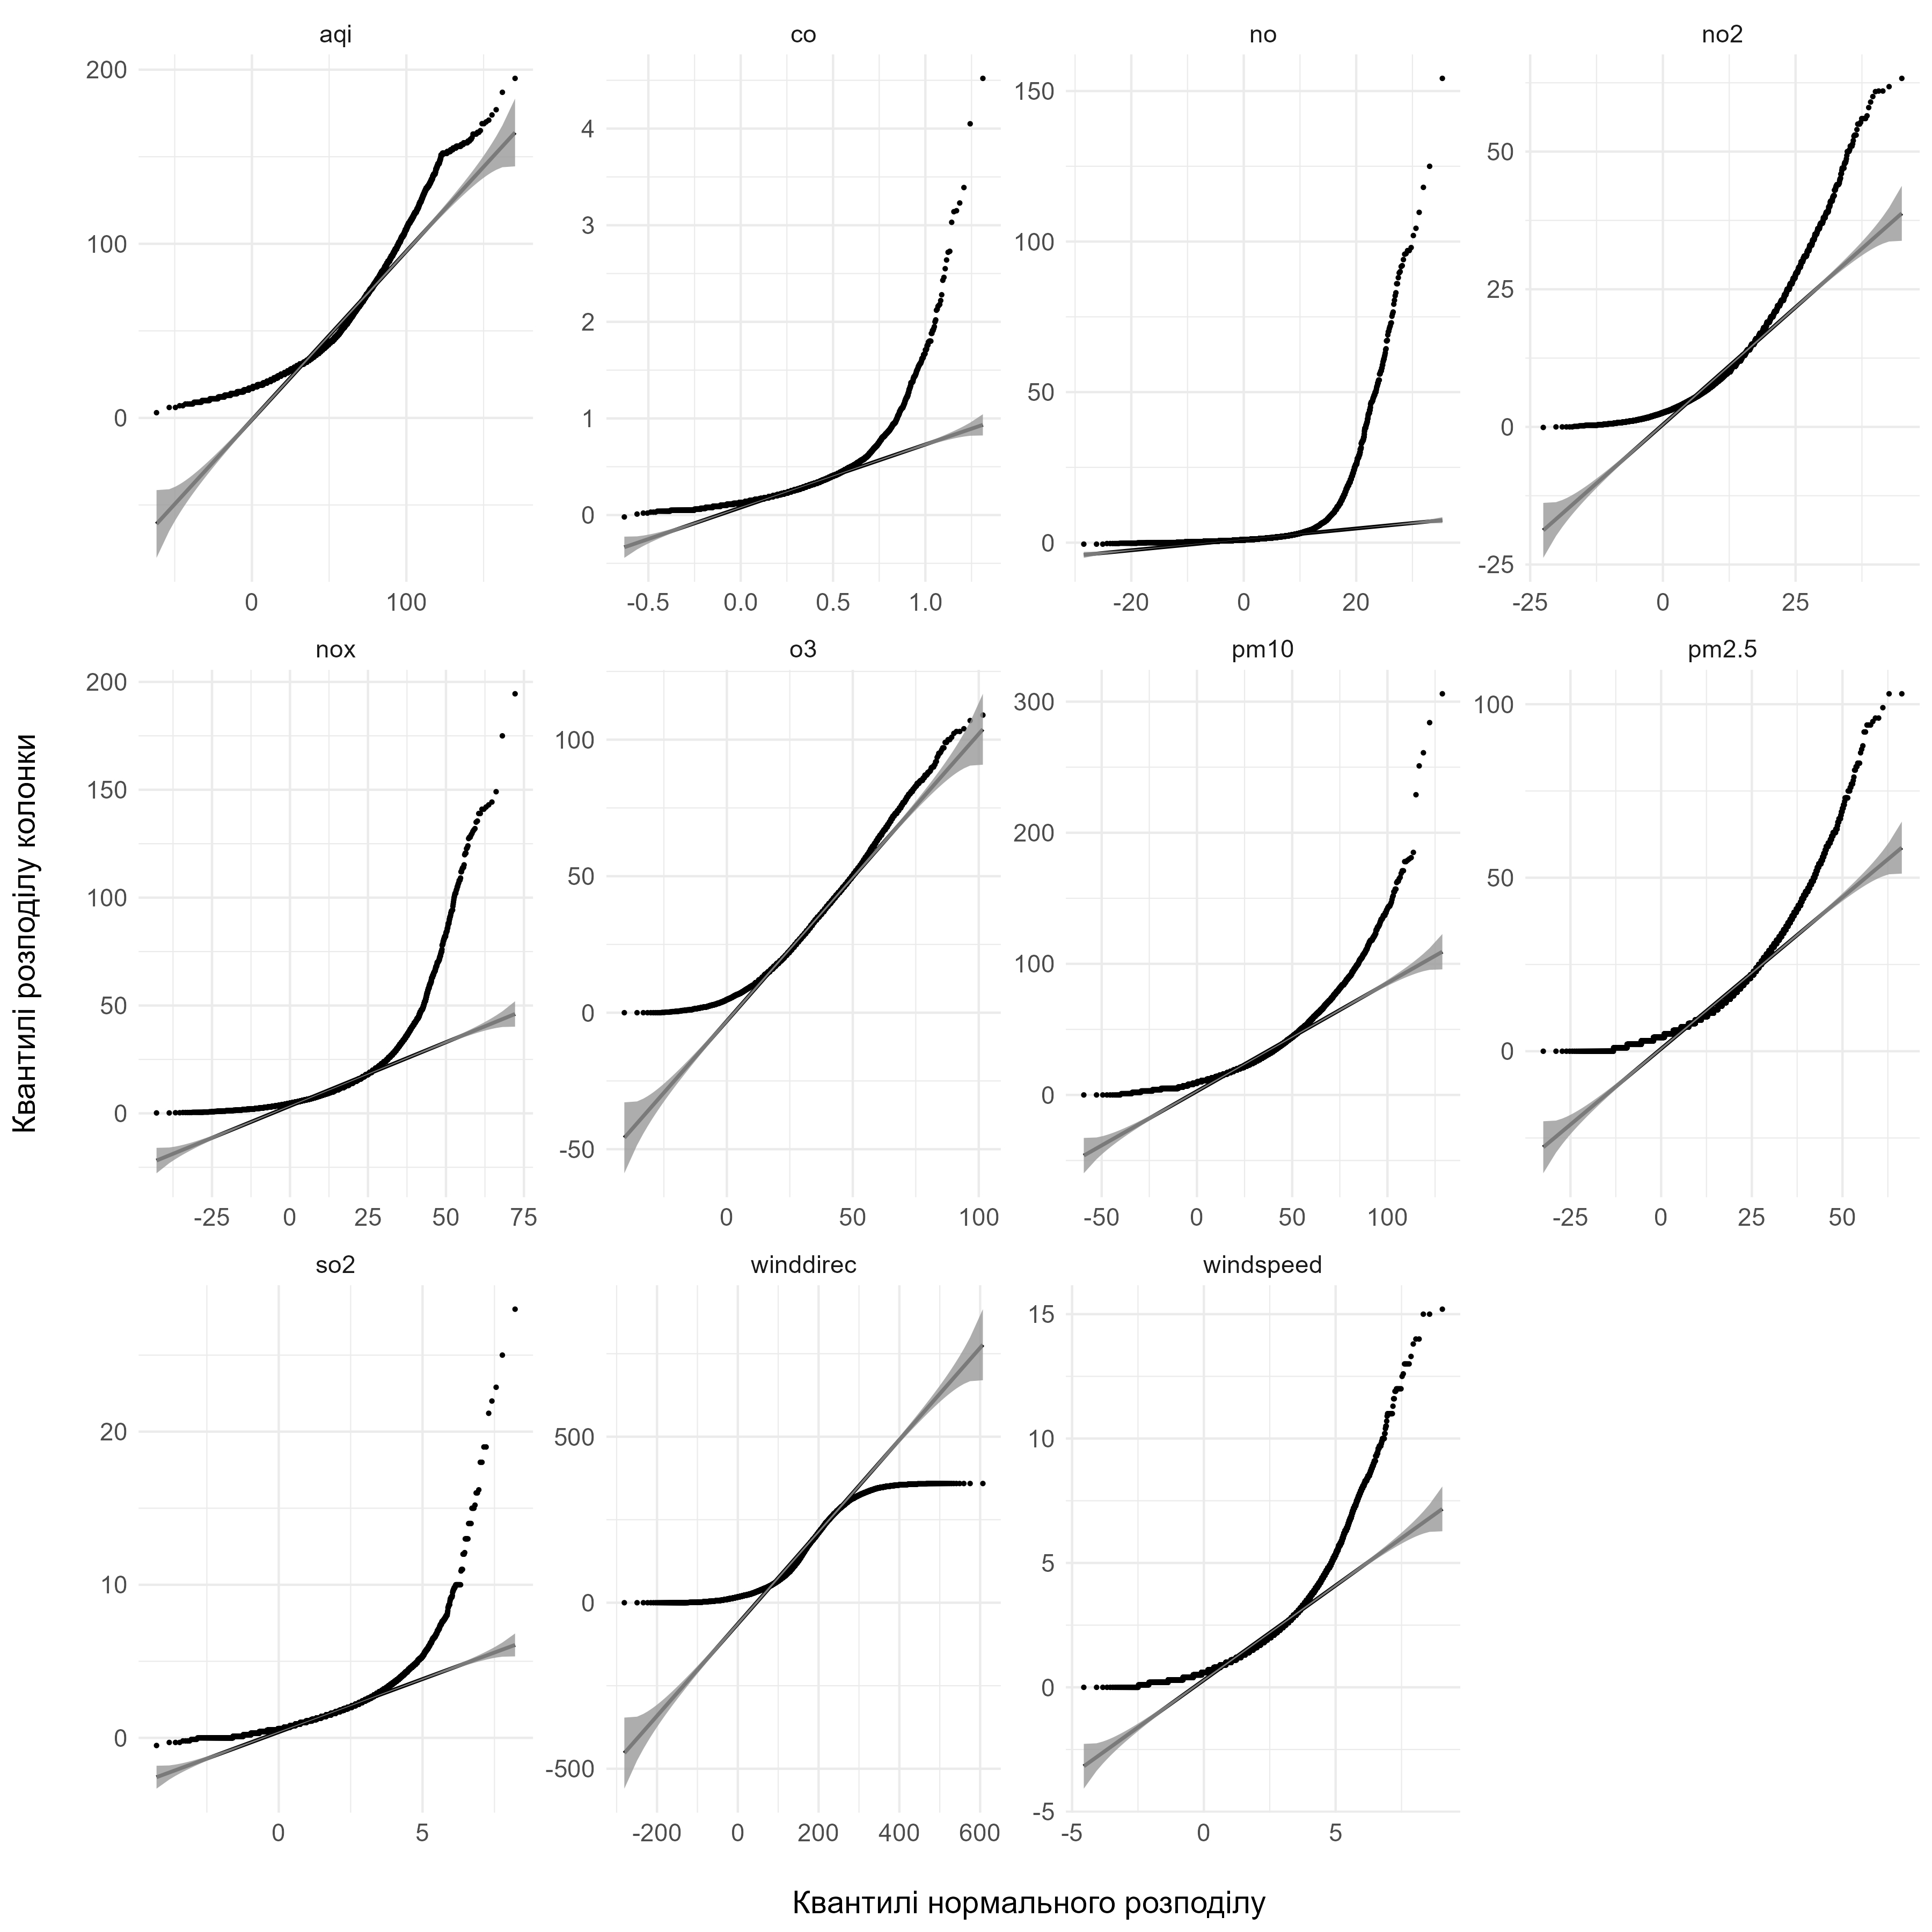
\includegraphics[width=5.5in]{plots/qq_tidy/qq.png}

    \pagebreak
    
    Розподіл змінних (крім winddirect) ближче до логнормального, ніж нормального:

    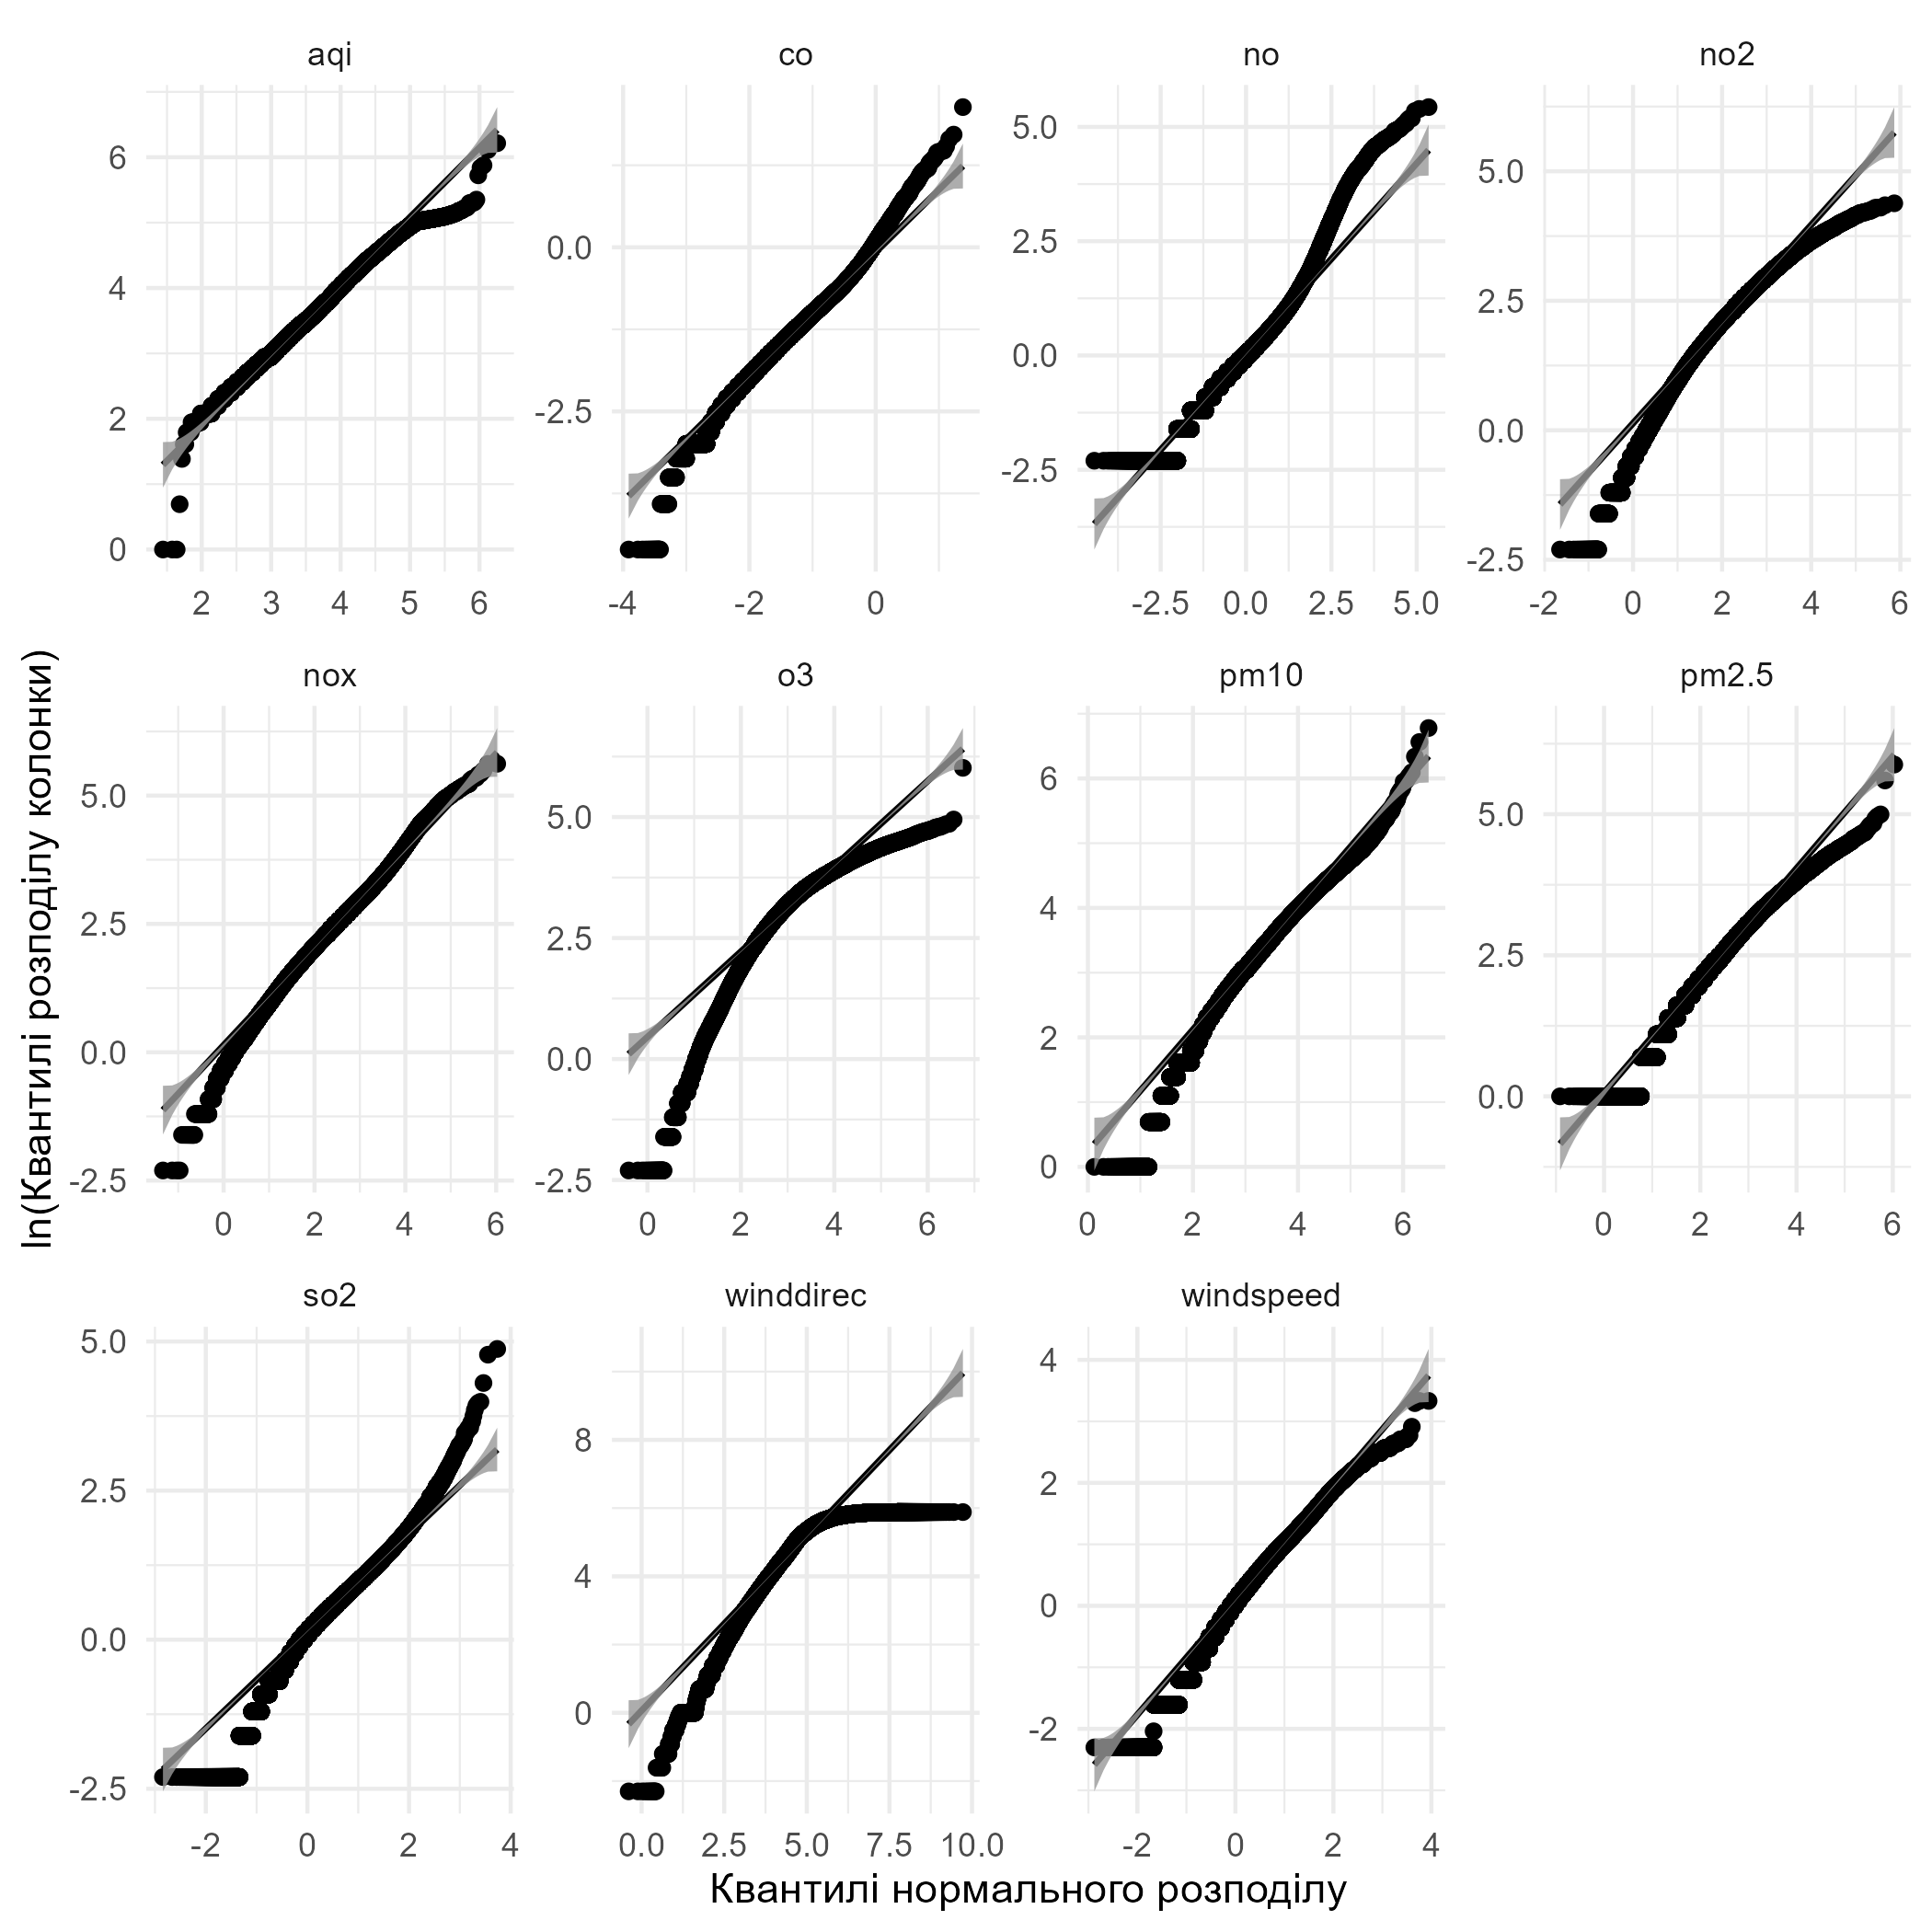
\includegraphics[width=6in]{plots/qq_tidy/qq-log.png}
    
    
\end{enumerate}

\pagebreak

\section{EDA}

\begin{enumerate}
    \item Чи впливає швидкість вітру (windspeed) на концентрацію частинок PM2.5 і PM10?
    
    \quad \textit{Був використаний trimmed набір даних}

    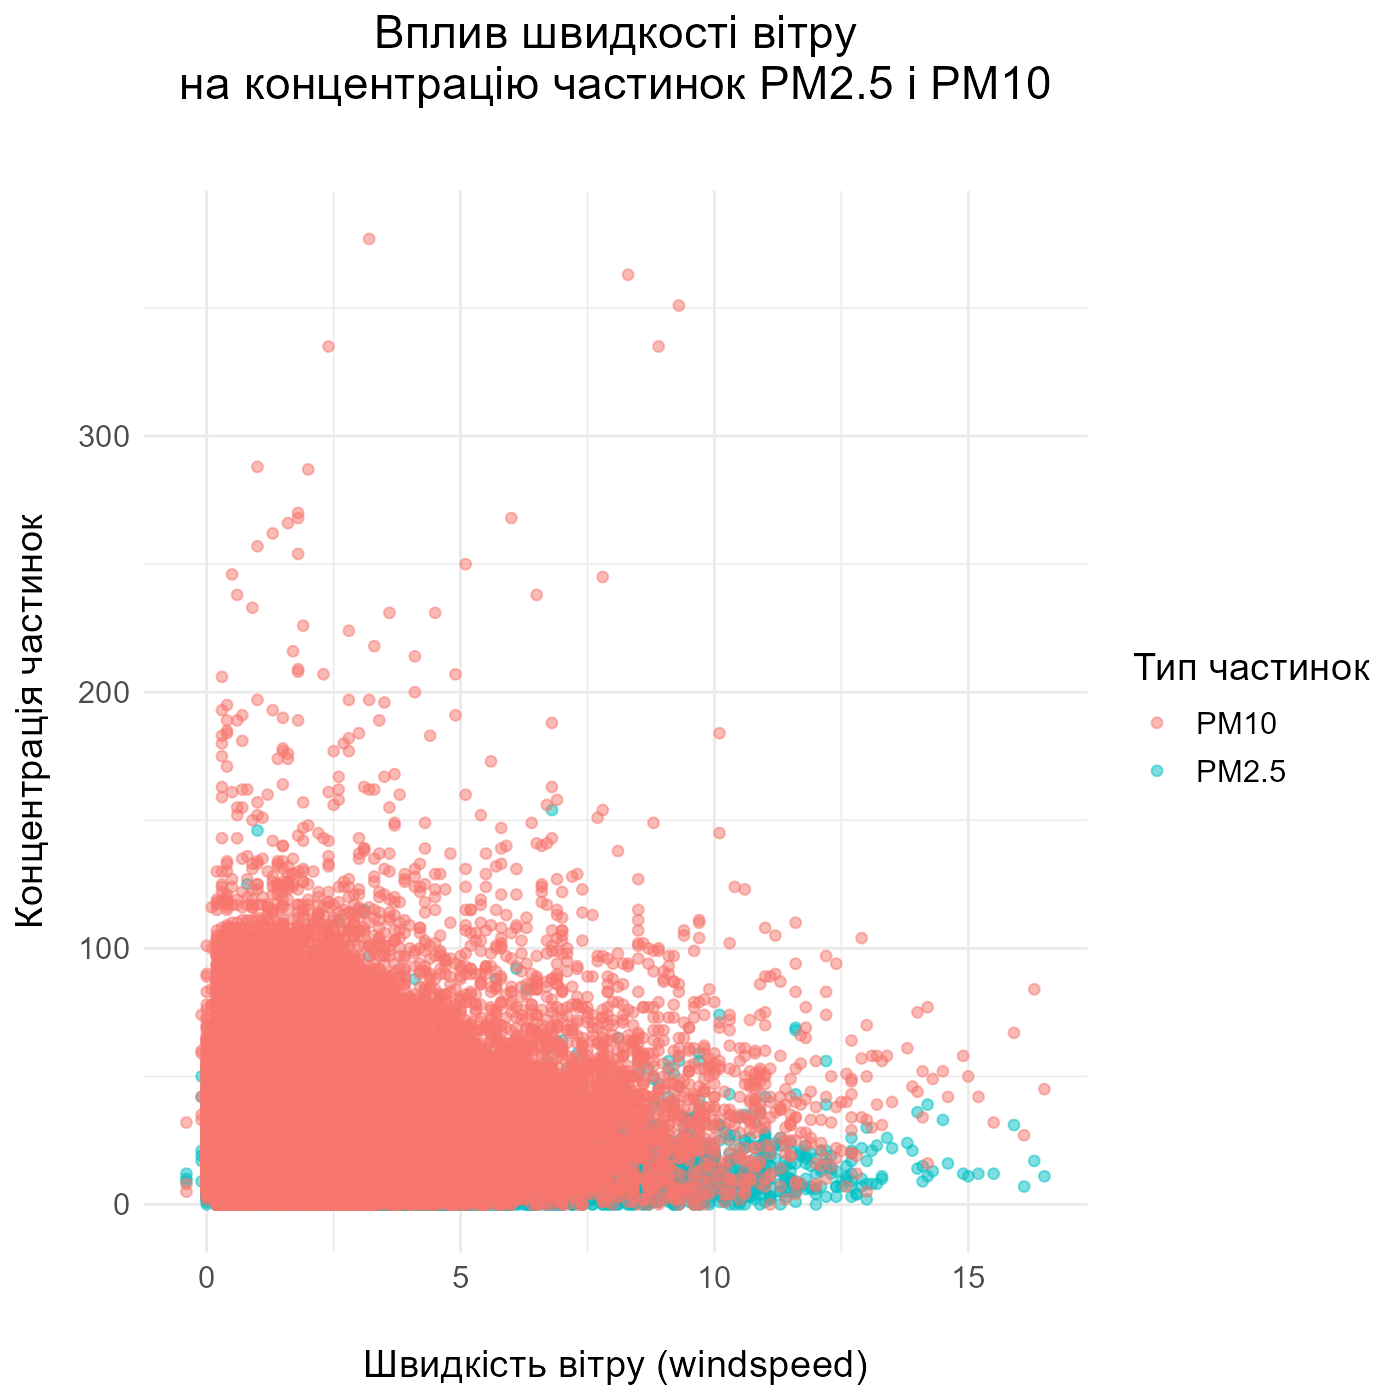
\includegraphics[width=6in]{plots/question1/wind_speed_vs_pm.png}

    Аналізуючи діагарму розсіювання, можна зазначити, що зі збільшенням швидкості вітру концентрації PM2.5, так і PM10 зменшуються.
    Розсіювання менше при високій швидкості вітру:
    \begin{itemize}
        \item При низьких швидкостях (0–5 м/с) спостерігається висока концентрація частинок і велика дисперсія.
        \item Починаючи з ~10 м/с, майже немає точок із високими концентраціями.
        \item PM10 (червоні точки) має більші значення концентрації, ніж PM2.5 (блакитні точки).
    \end{itemize}
    Тобто вітер розсіює тверді частинки в повітрі, тому при сильному вітрі повітря «чистіше». Обидва типи частинок зменшуються при зростанні швидкості вітру.

    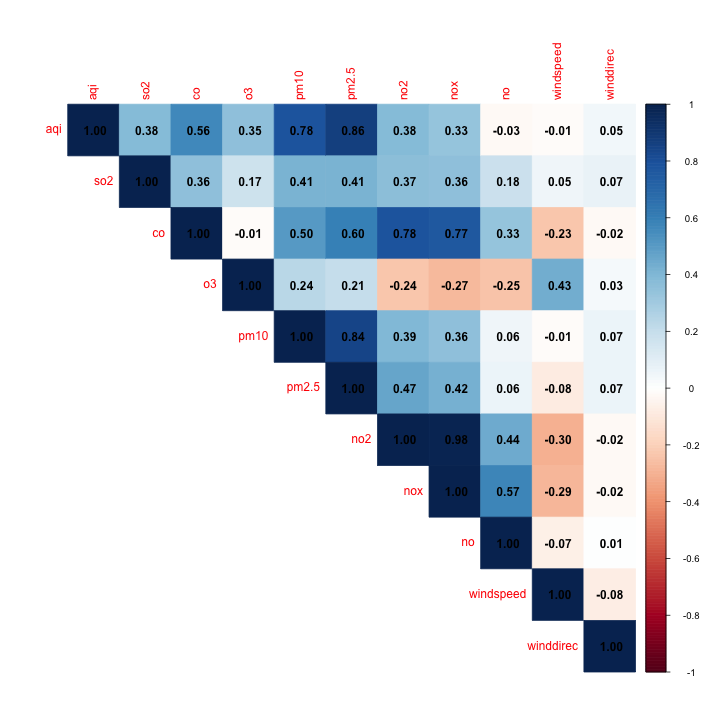
\includegraphics[width=6in]{plots/question1/corr_matrix_plot.png}

    Рядки та стовпці: різні забруднювачі й погодні фактори. Значення — кореляції Пірсона (від -1 до 1).
    \begin{itemize}
        \item PM2.5

        Зі швидкістю вітру: -0.08 (слабка негативна);

        З PM10: +0.84 — сильна кореляція (часто зростають разом);

        З $NO_2$: +0.46, CO: +0.60 — середня позитивна.
    \item PM10
 
        Зі швидкістю вітру: -0.06 (слабка негативна)

        З PM2.5: +0.84

        З $NO_2$: +0.39, $CO$: +0.50

    \item Швидкість вітру (windspeed)
    \item 
        З $PM_{10}$: -0.06, з $PM_{2.5}$: -0.08 — слабкий негативний зв'язок.

        З $NO_2$: -0.30, $NO_x$: -0.29 — тут зв'язок сильніший (тобто вітер сильніше зменшує газоподібні забруднювачі, ніж тверді частинки).

        З $O_3$: +0.43 — вітер, ймовірно, підвищує рівень озону (через хімічні реакції чи перемішування повітря).
    \end{itemize}   

    Підсумовуючи можна сказати,що $PM_{2.5}$ і $ PM_{10}$ слабко негативно корелюють зі швидкістю вітру, що підтверджує попередній графік.
    Проте вплив вітру на газоподібні забруднювачі ($NO_2$, $NO_x$) є сильнішим. 
    Це може бути через більшу мобільність газів у порівнянні з твердими частинками.

    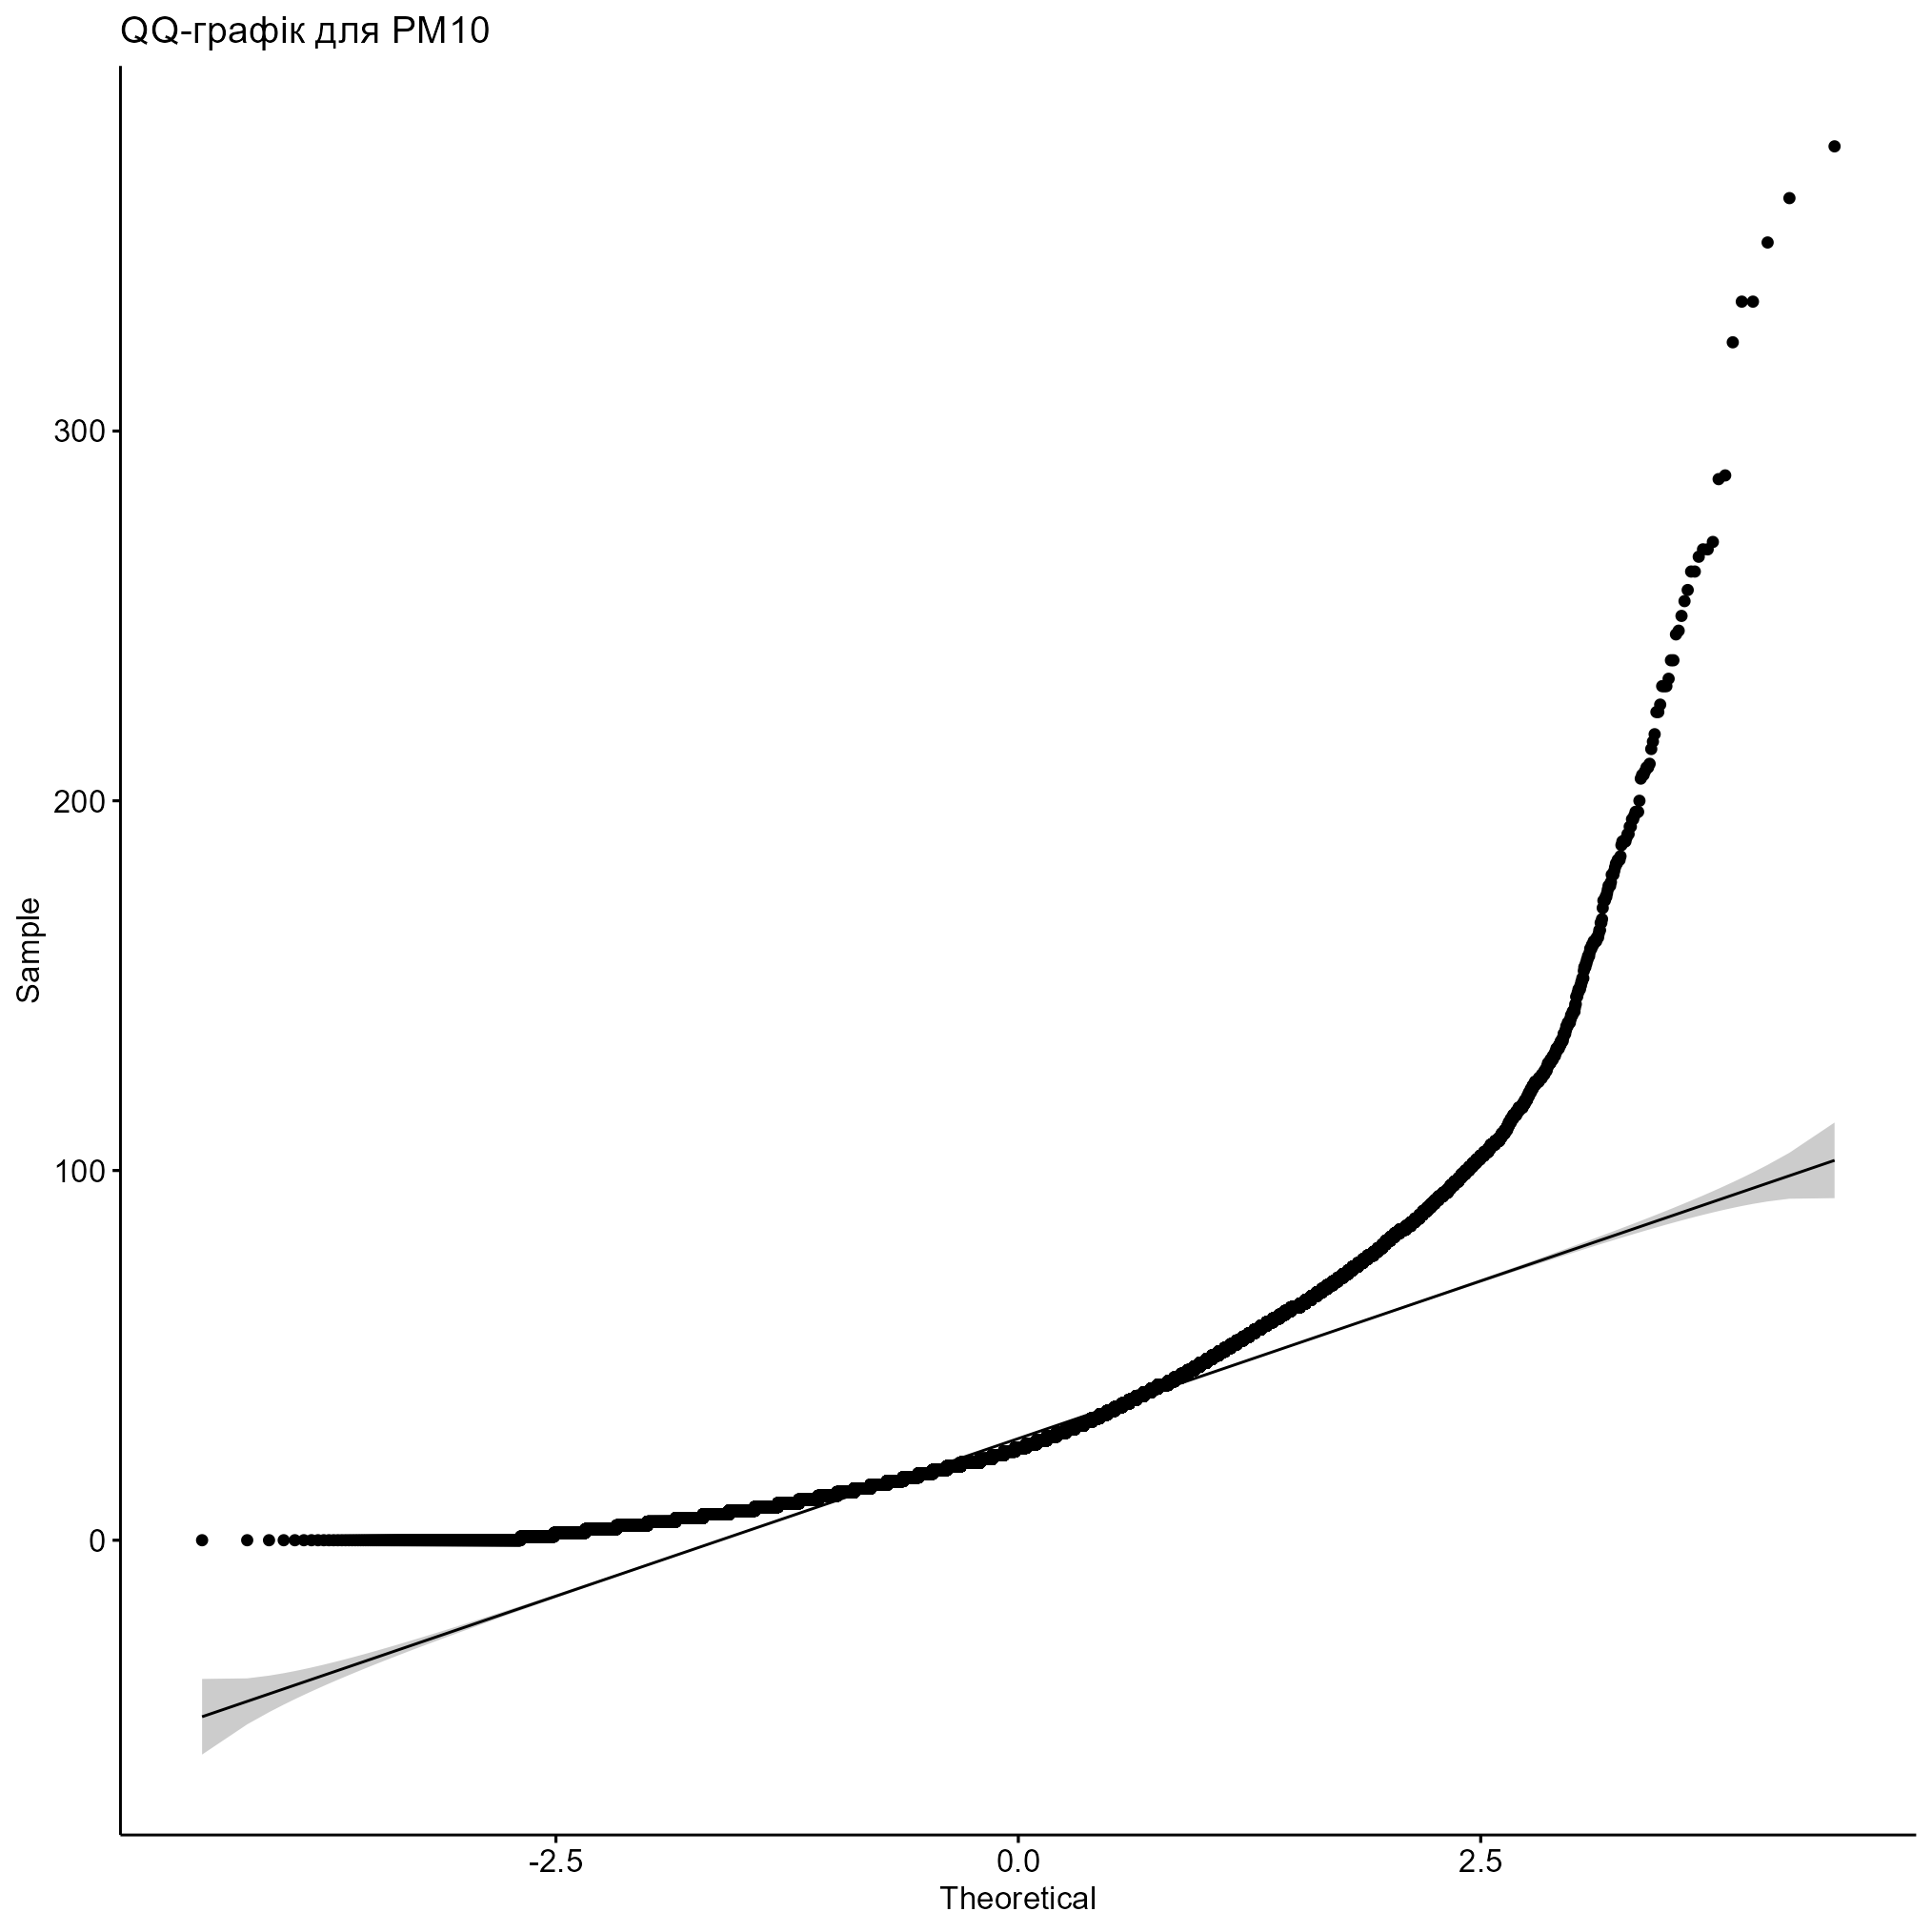
\includegraphics[width=6in]{plots/question1/qq_pm10.png}
    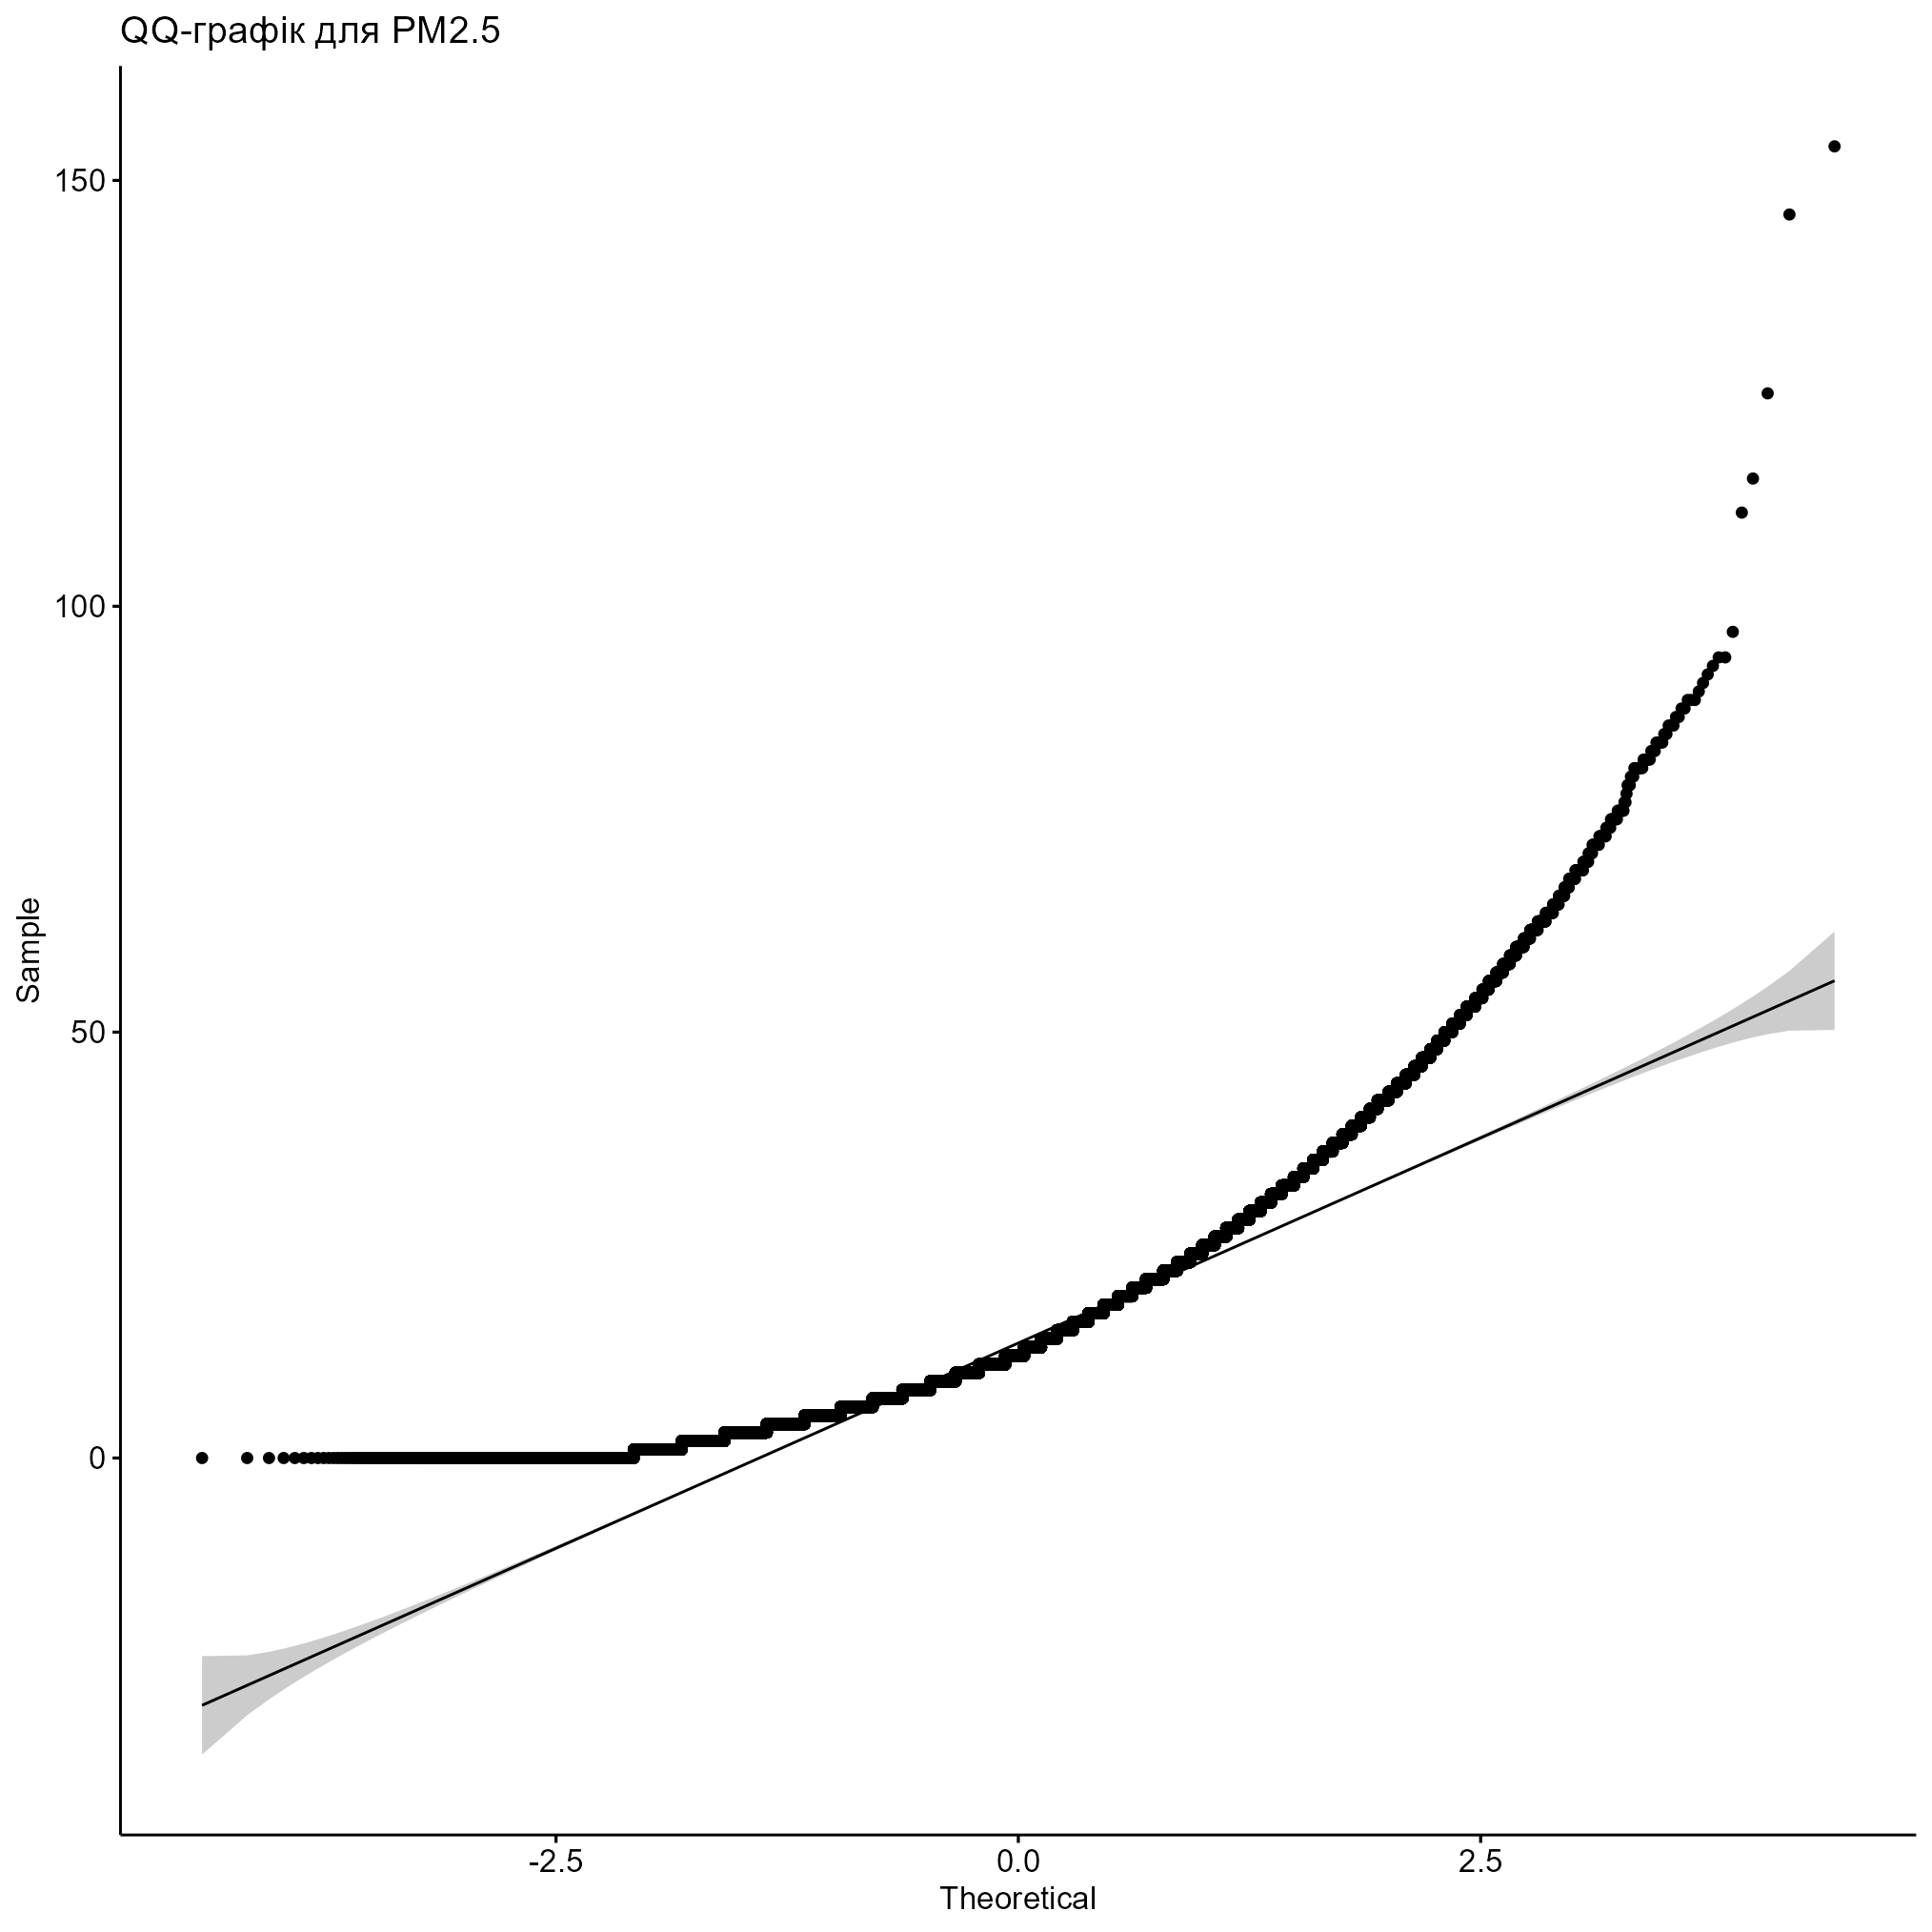
\includegraphics[width=6in]{plots/question1/qq_pm2_5.png}
    QQ-графіки твердих частинок пдозволяють відслідкувати викиди по вимірам. Тобто від 0 до 200 має нормальний розподіл, потім починаєтсья розсіювання.
    \item Як зміни в концентрації  ($O_3$)  та $SO_2$ впливають на загальний рівень забруднення повітря (AQI)?
    
    \quad \textit{Був використаний trimmed набір даних}

    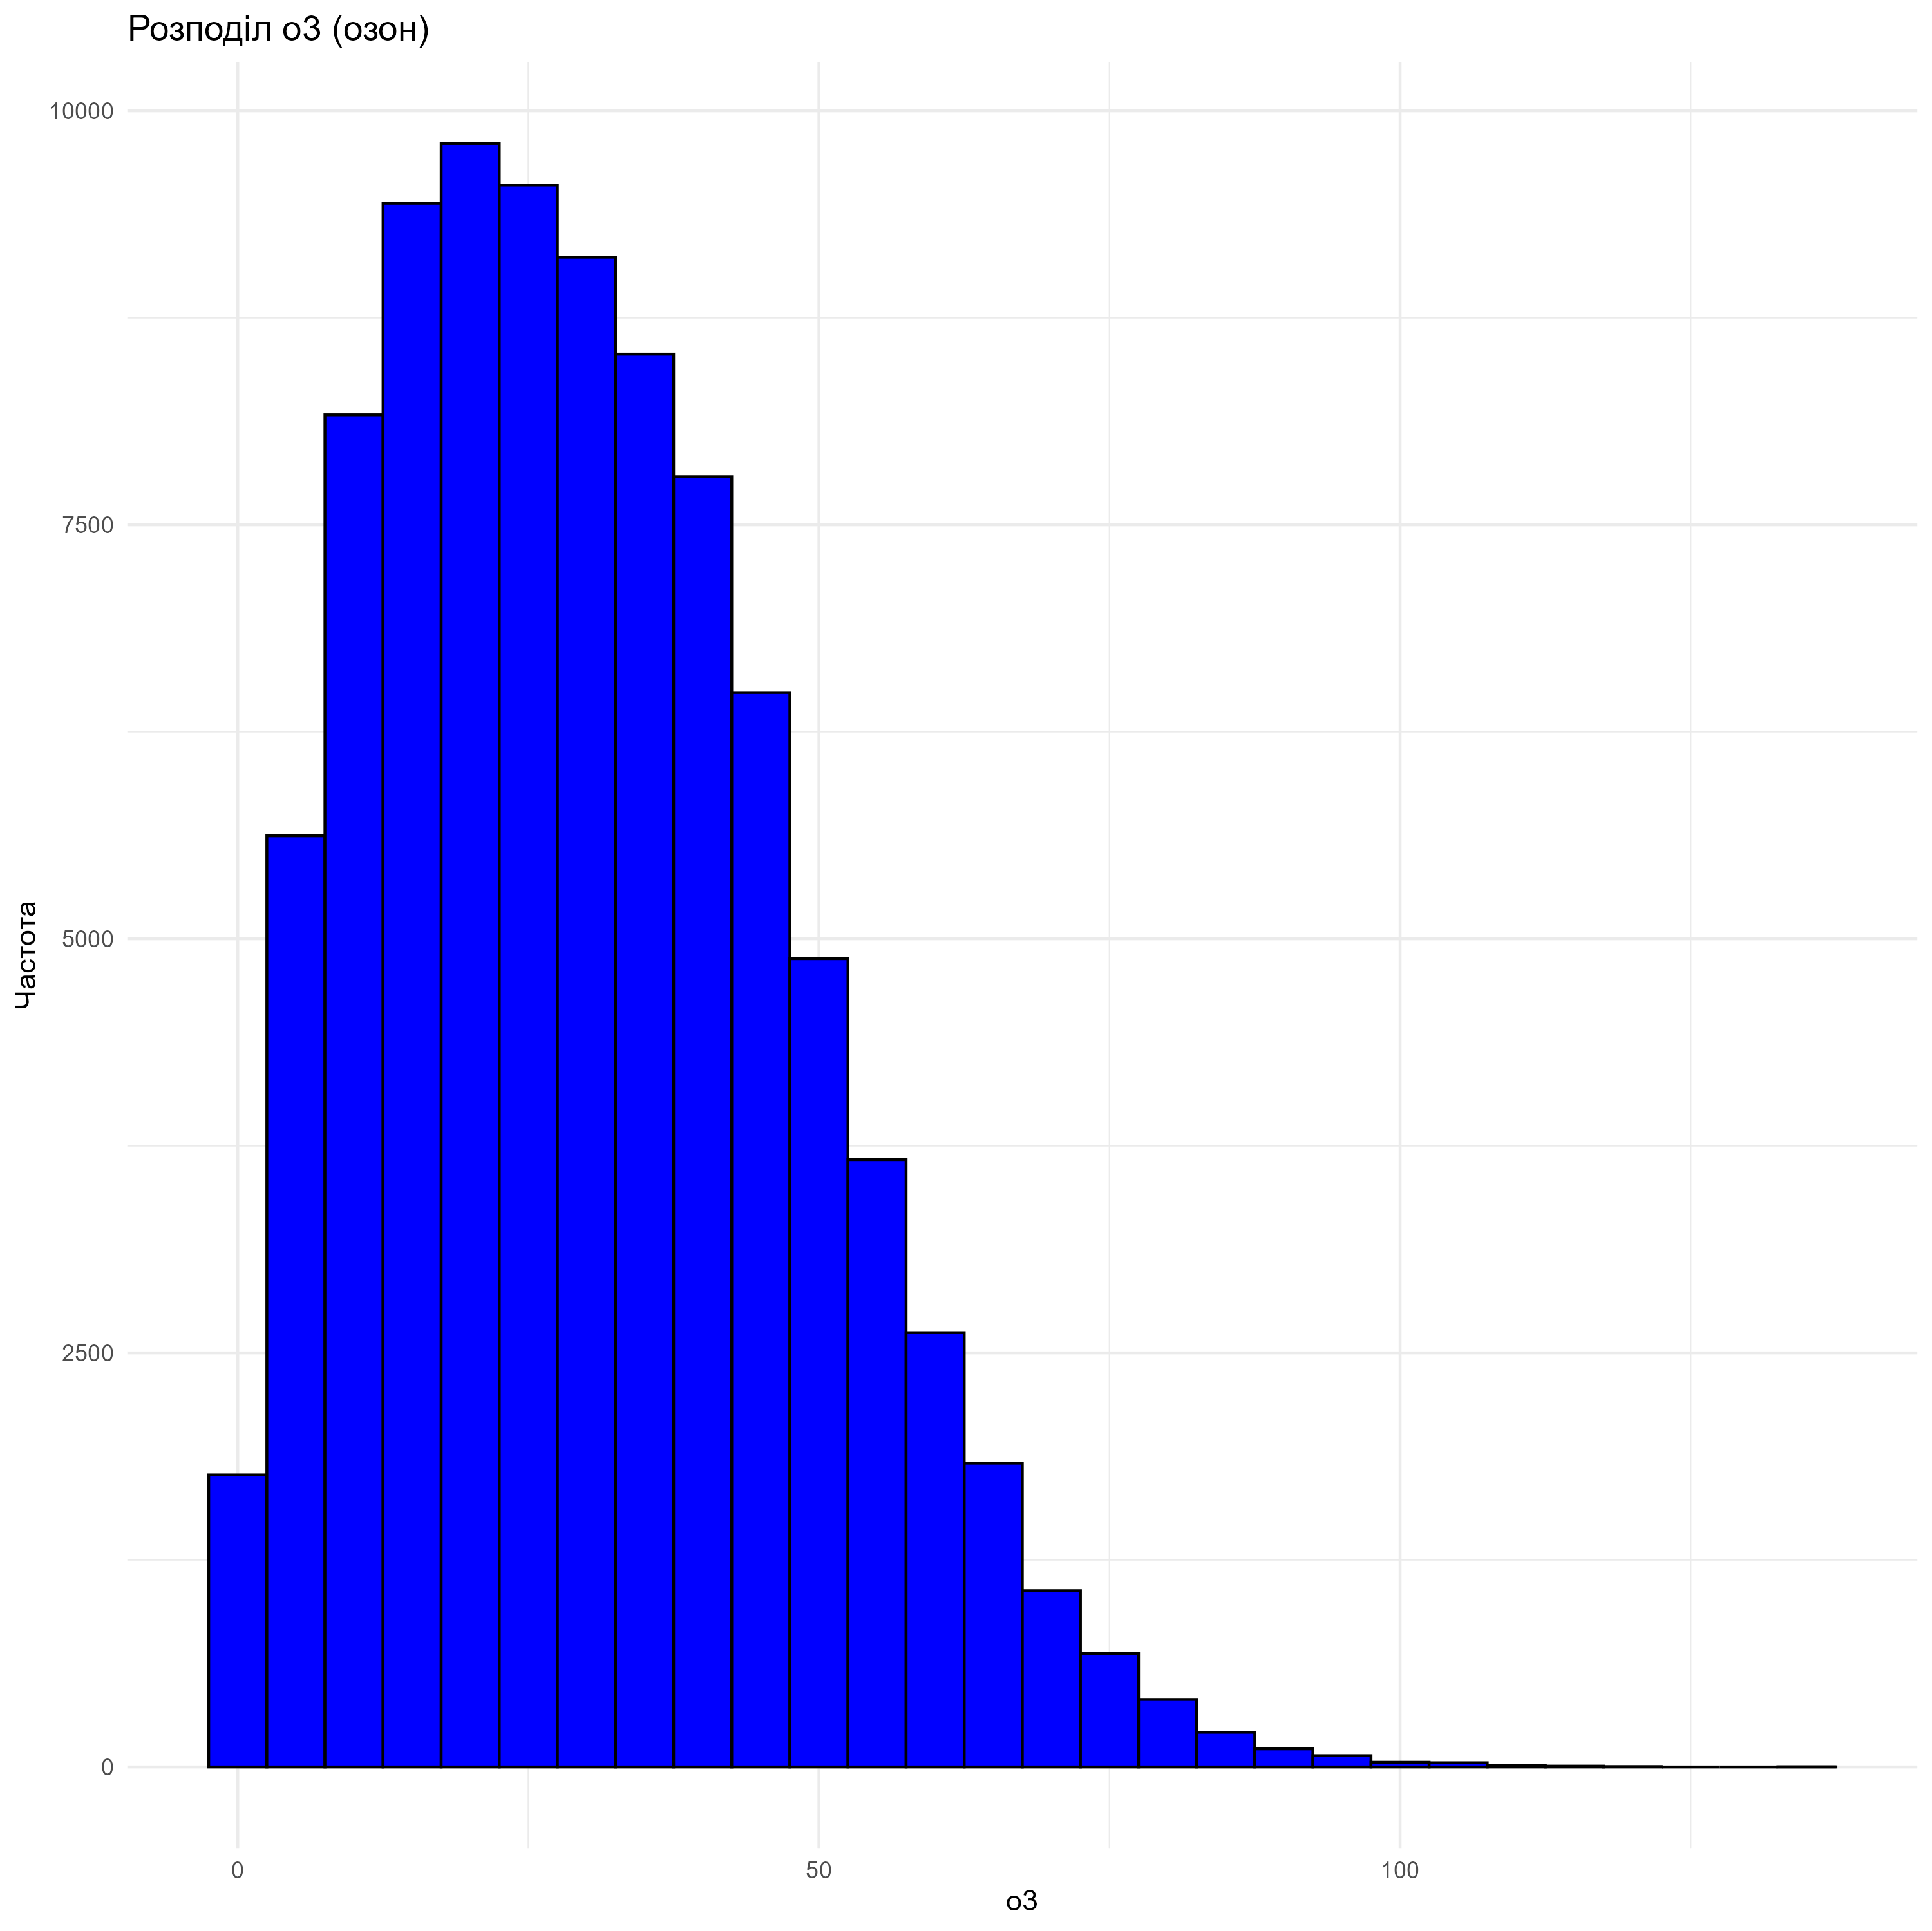
\includegraphics[width=6in]{plots/question2/o3_plot.png}
    
    Гістограма показує, що більшість значень $O_3$ знаходяться в межах 0-50 одиниць, а більш високі концентрації трапляються рідко.
    Це підтверджує, що озон зазвичай має помірний рівень, але все ж може впливати на AQI, особливо за високих значень.
    
    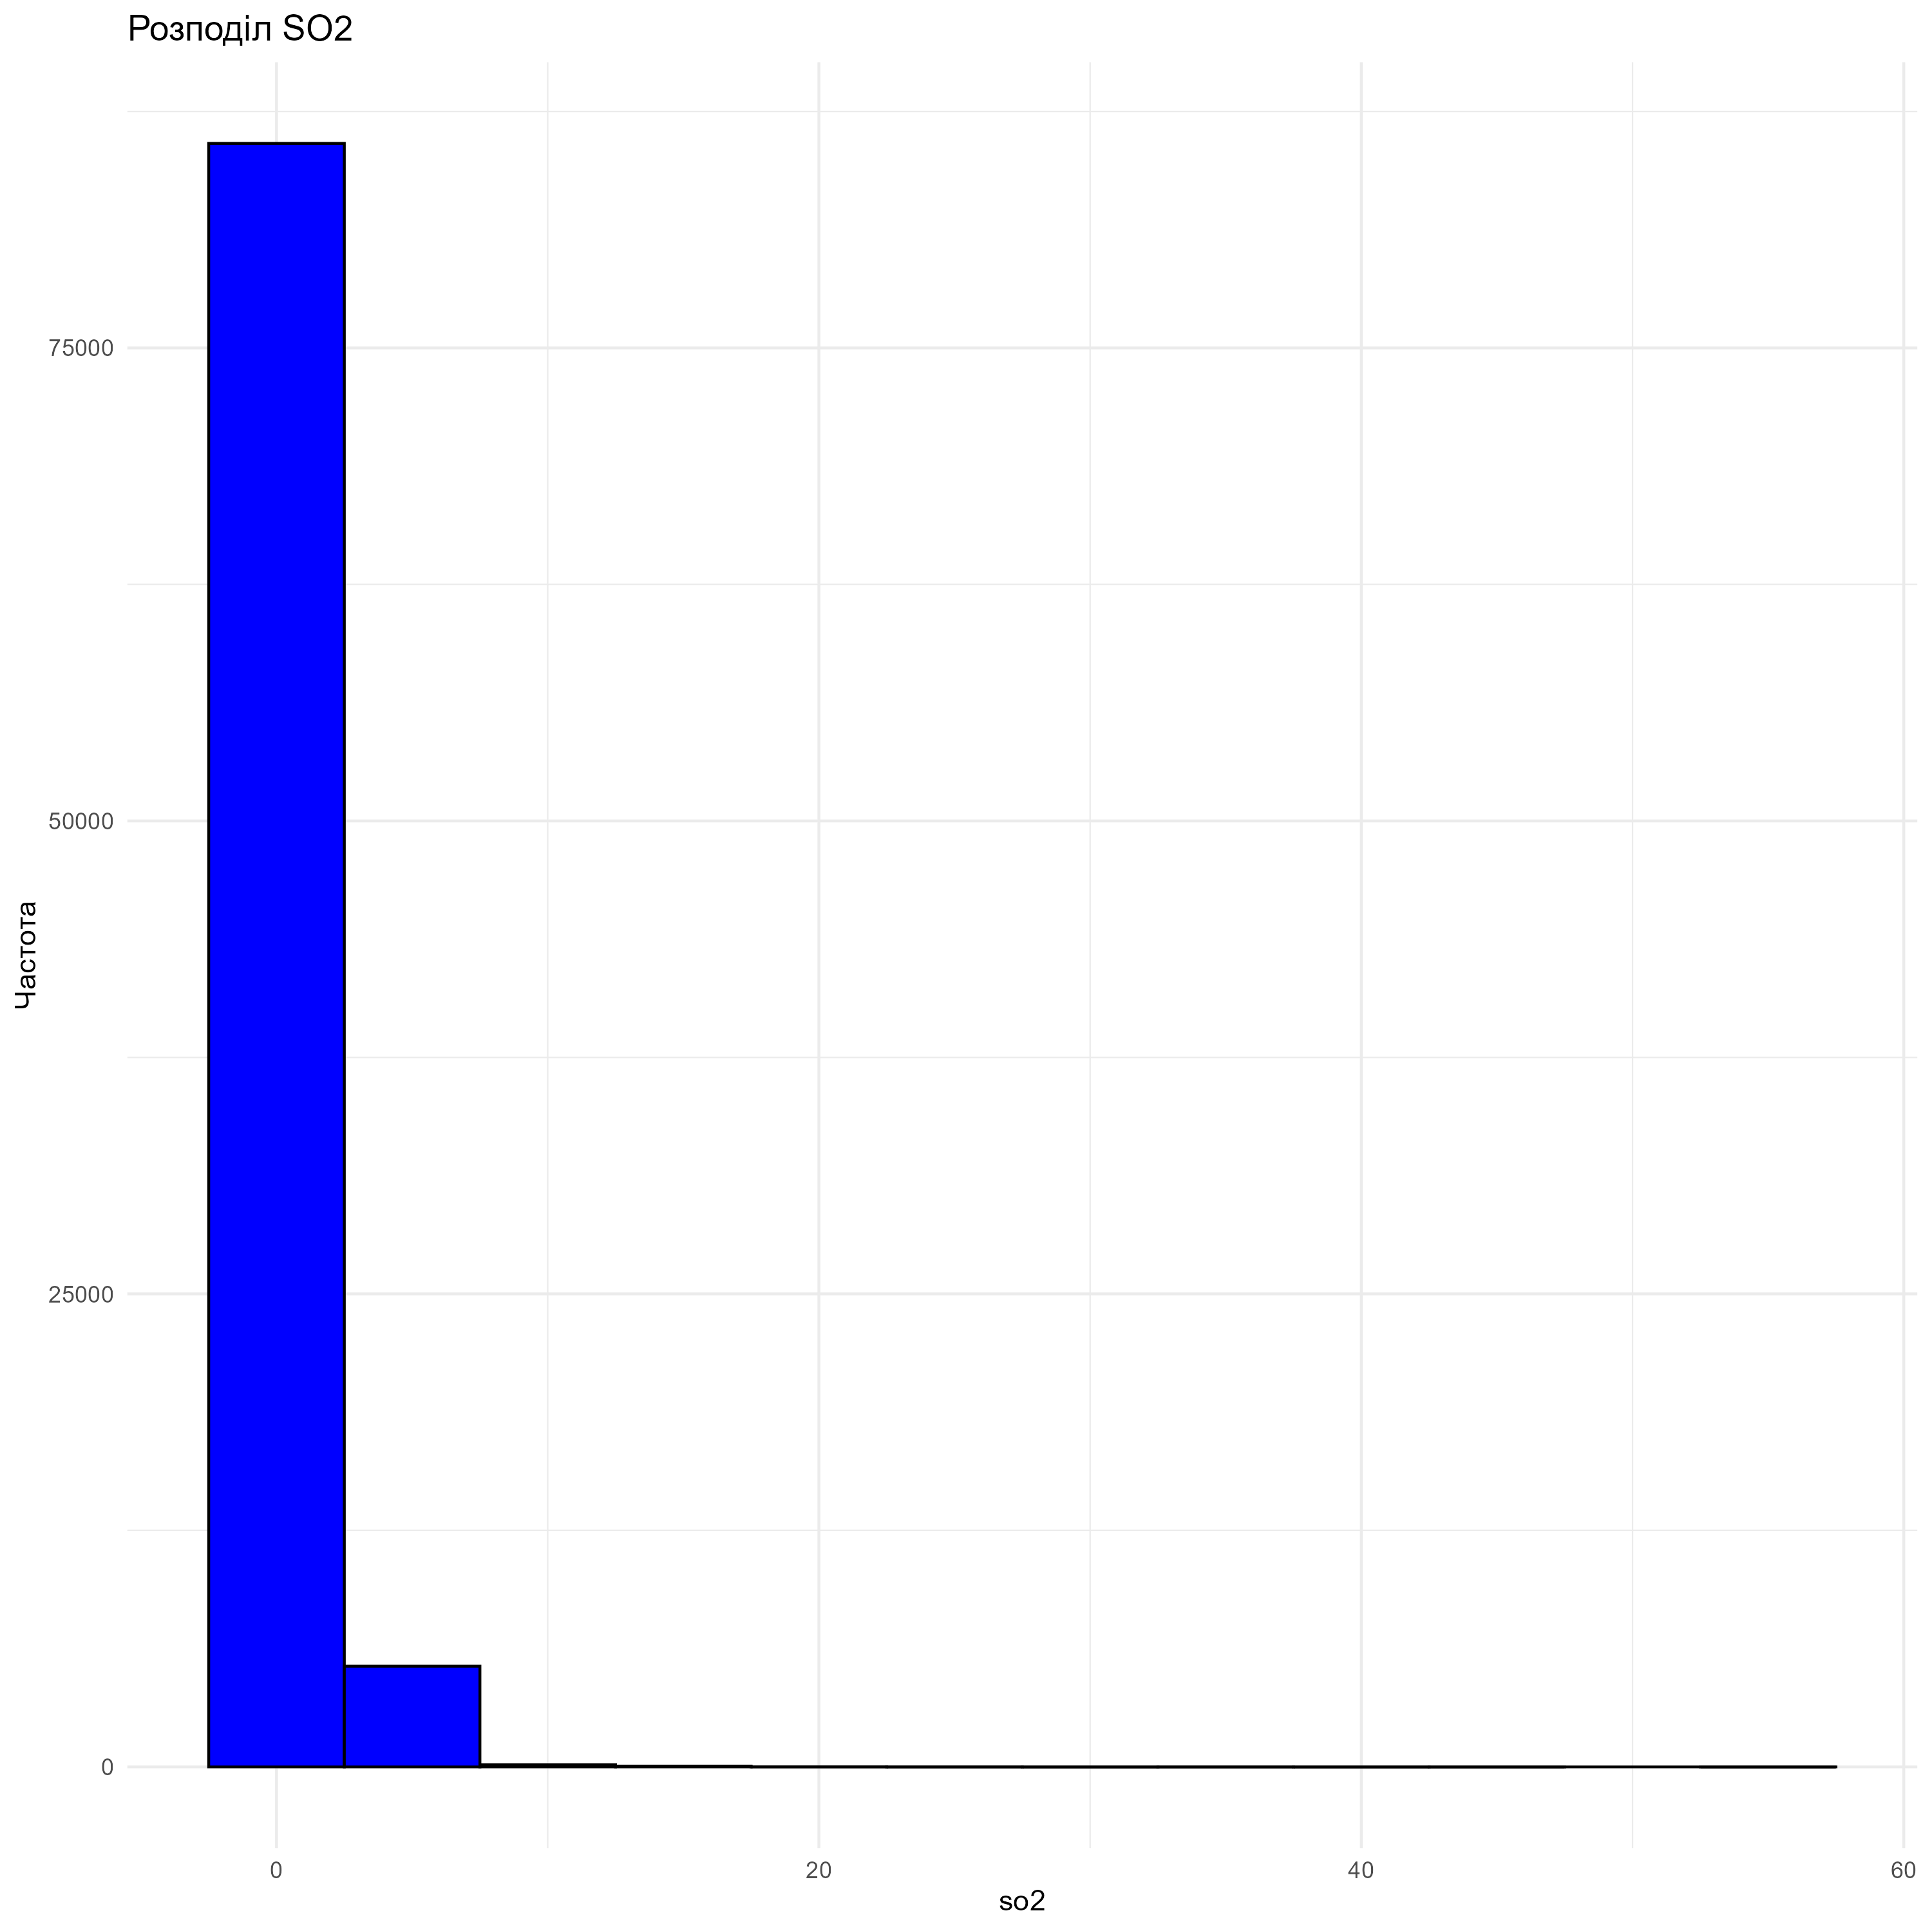
\includegraphics[width=6in]{plots/question2/so2_plot.png}
    
    Гістограма показує, що більшість значень $SO_2$ дуже малі (близькі до нуля).
    Це може свідчити про незначний внесок $SO_2$ у загальний рівень забруднення AQI у вибраних даних.   
    
    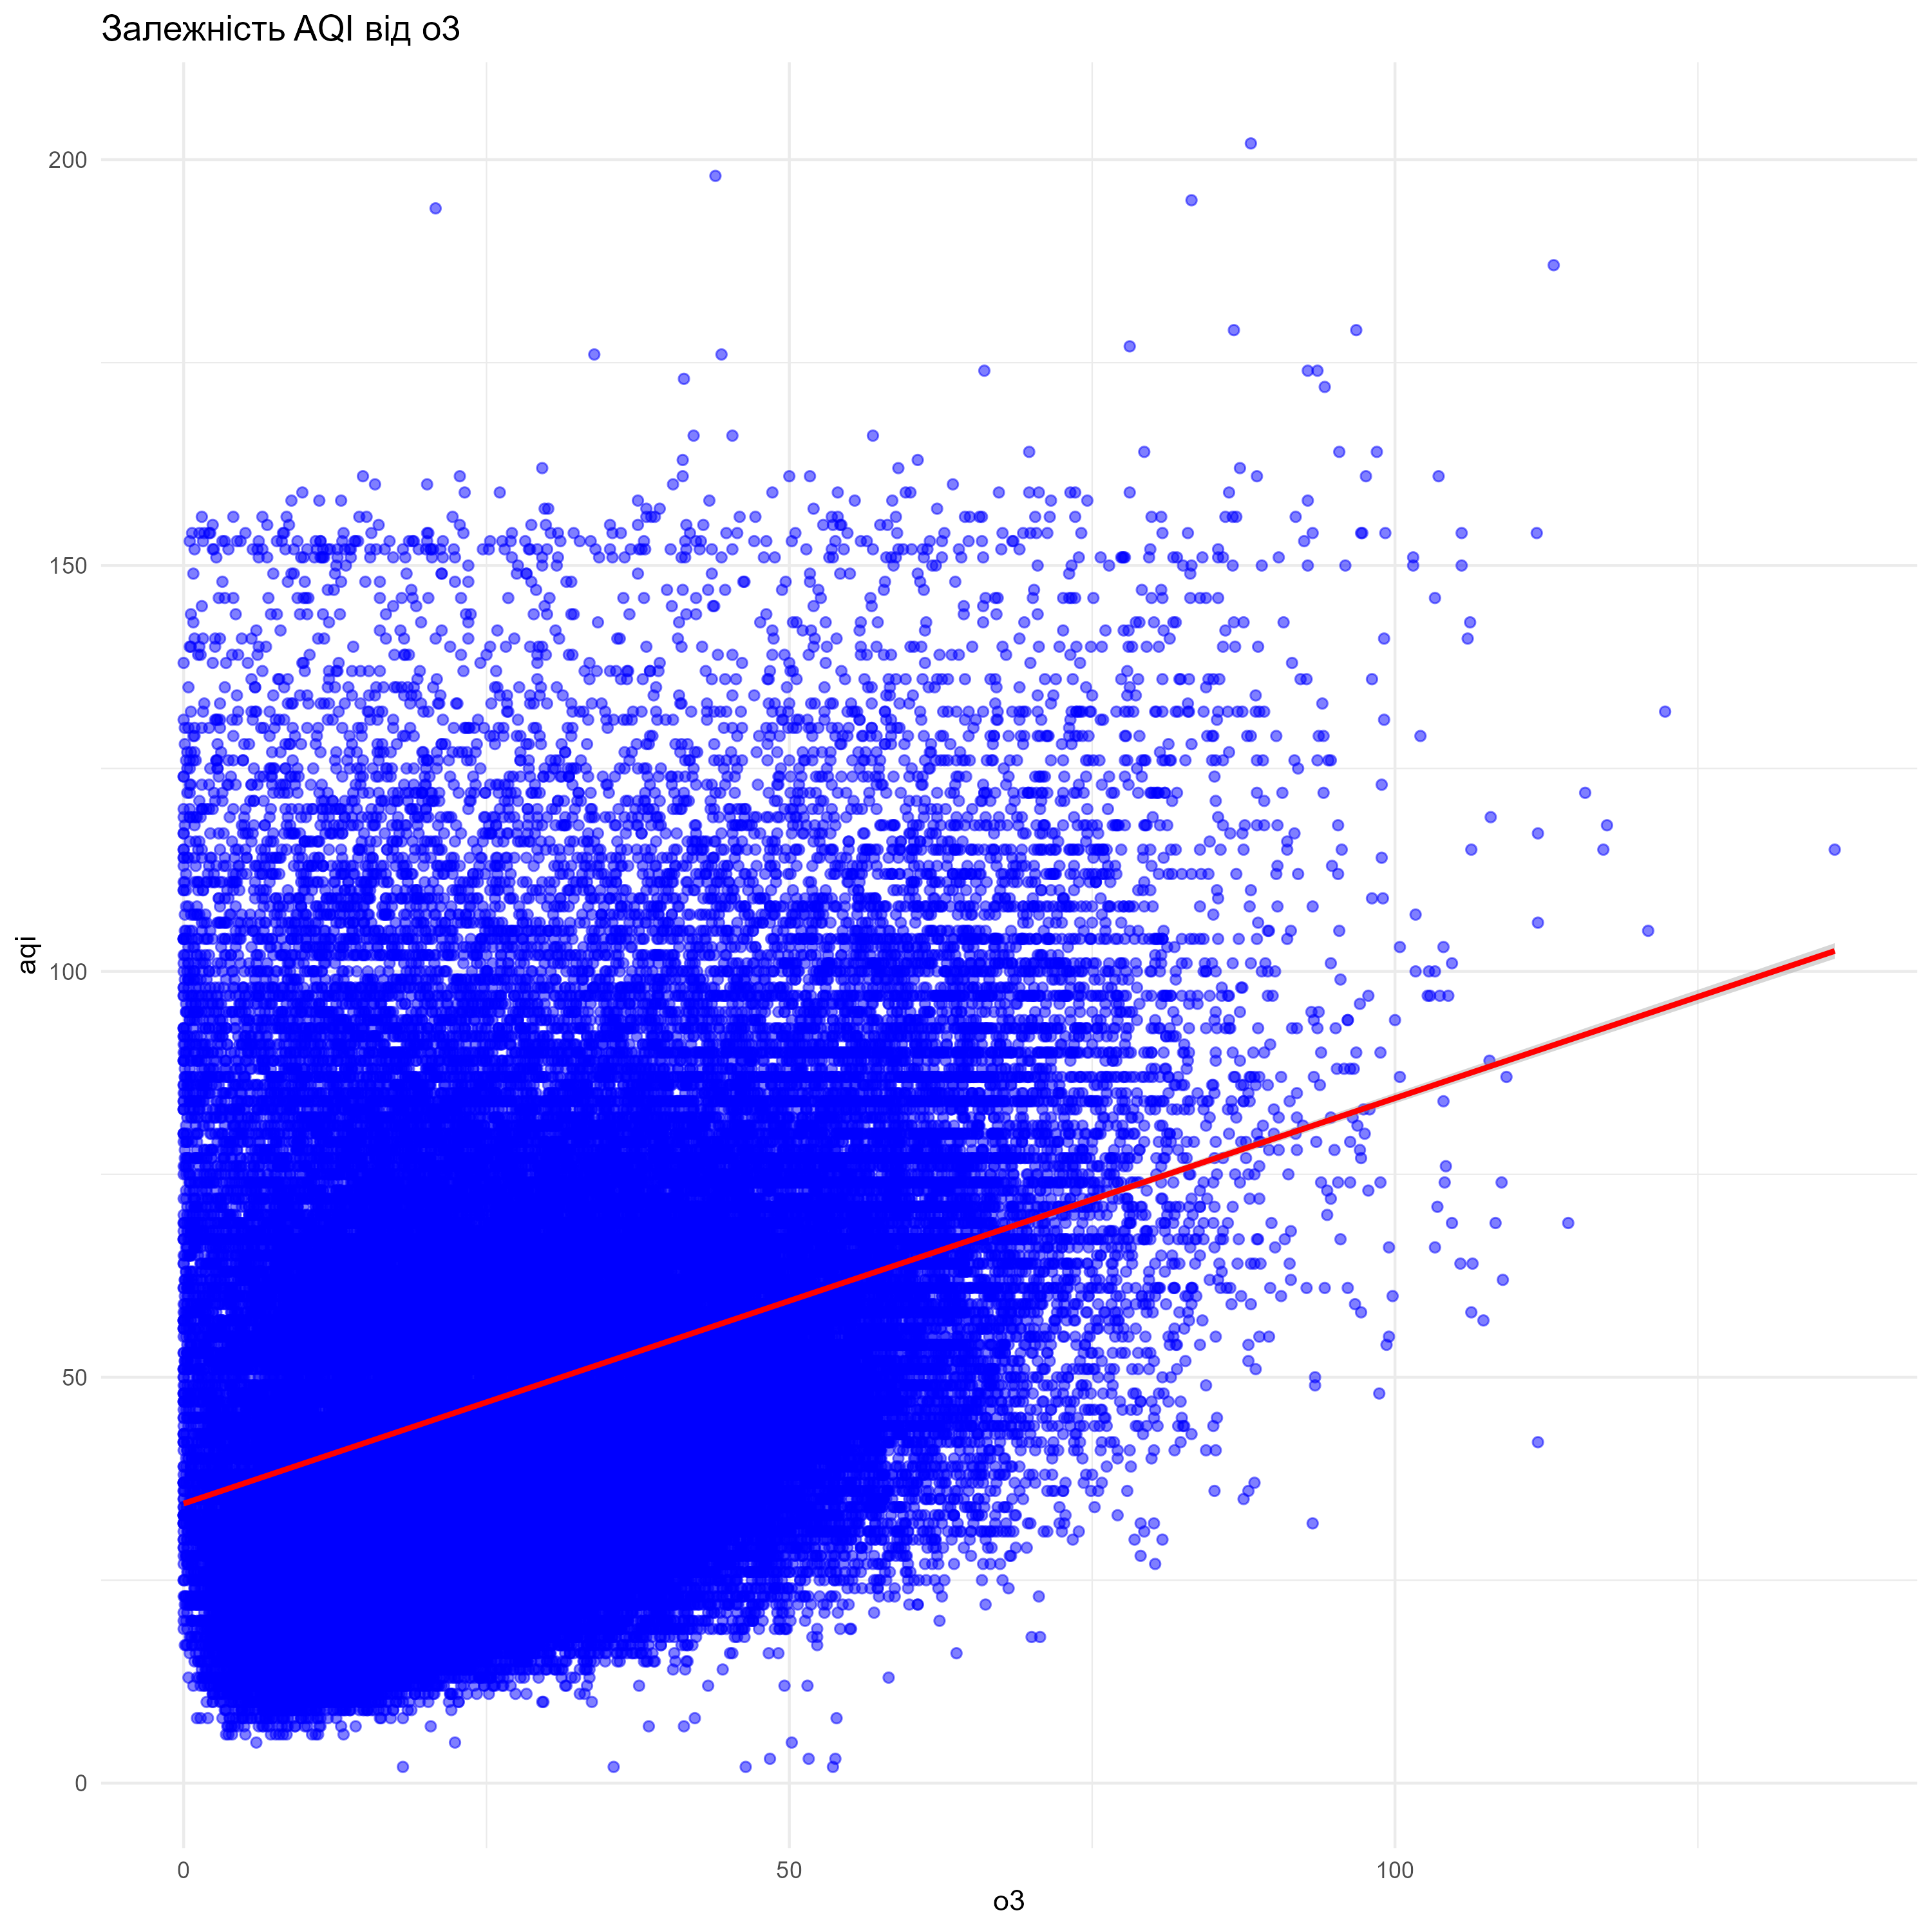
\includegraphics[width=6in]{plots/question2/scatter_plot.png}
    
    Спостерігається позитивна залежність між концентрацією $O_3$ та AQI: зростання озону супроводжується збільшенням індексу забруднення.
    Проте розсіювання значень значне, що може вказувати на вплив інших чинників.
    
    \begin{center}
    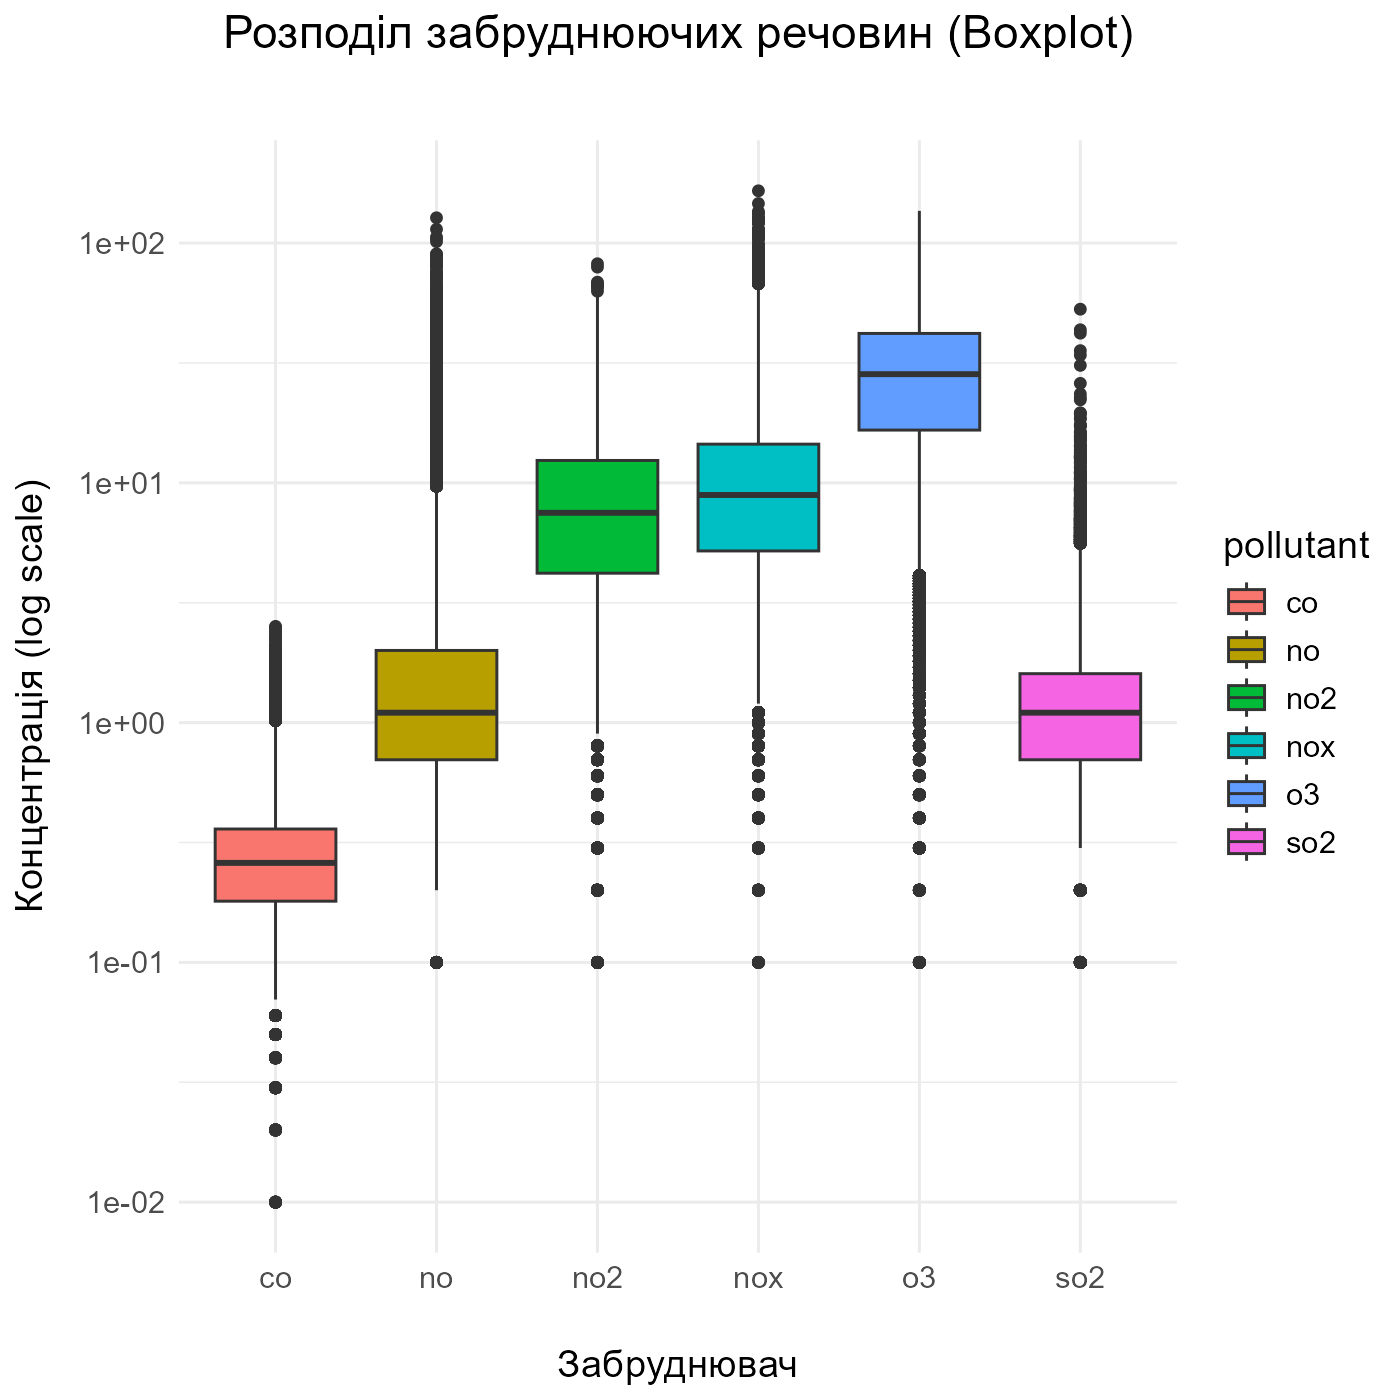
\includegraphics[width=6in]{plots/question2/boxplot_pollutants.png}
    \end{center}

    Спостерігається підвищена концентрація $O_3$ та відповідно відносно не значна $SO_2$.
    
    \item Як змінюється якість повітря (status) протягом доби в різних районах?
    
    \quad \textit{Був використаний tidy набір даних}

    \begin{center}
    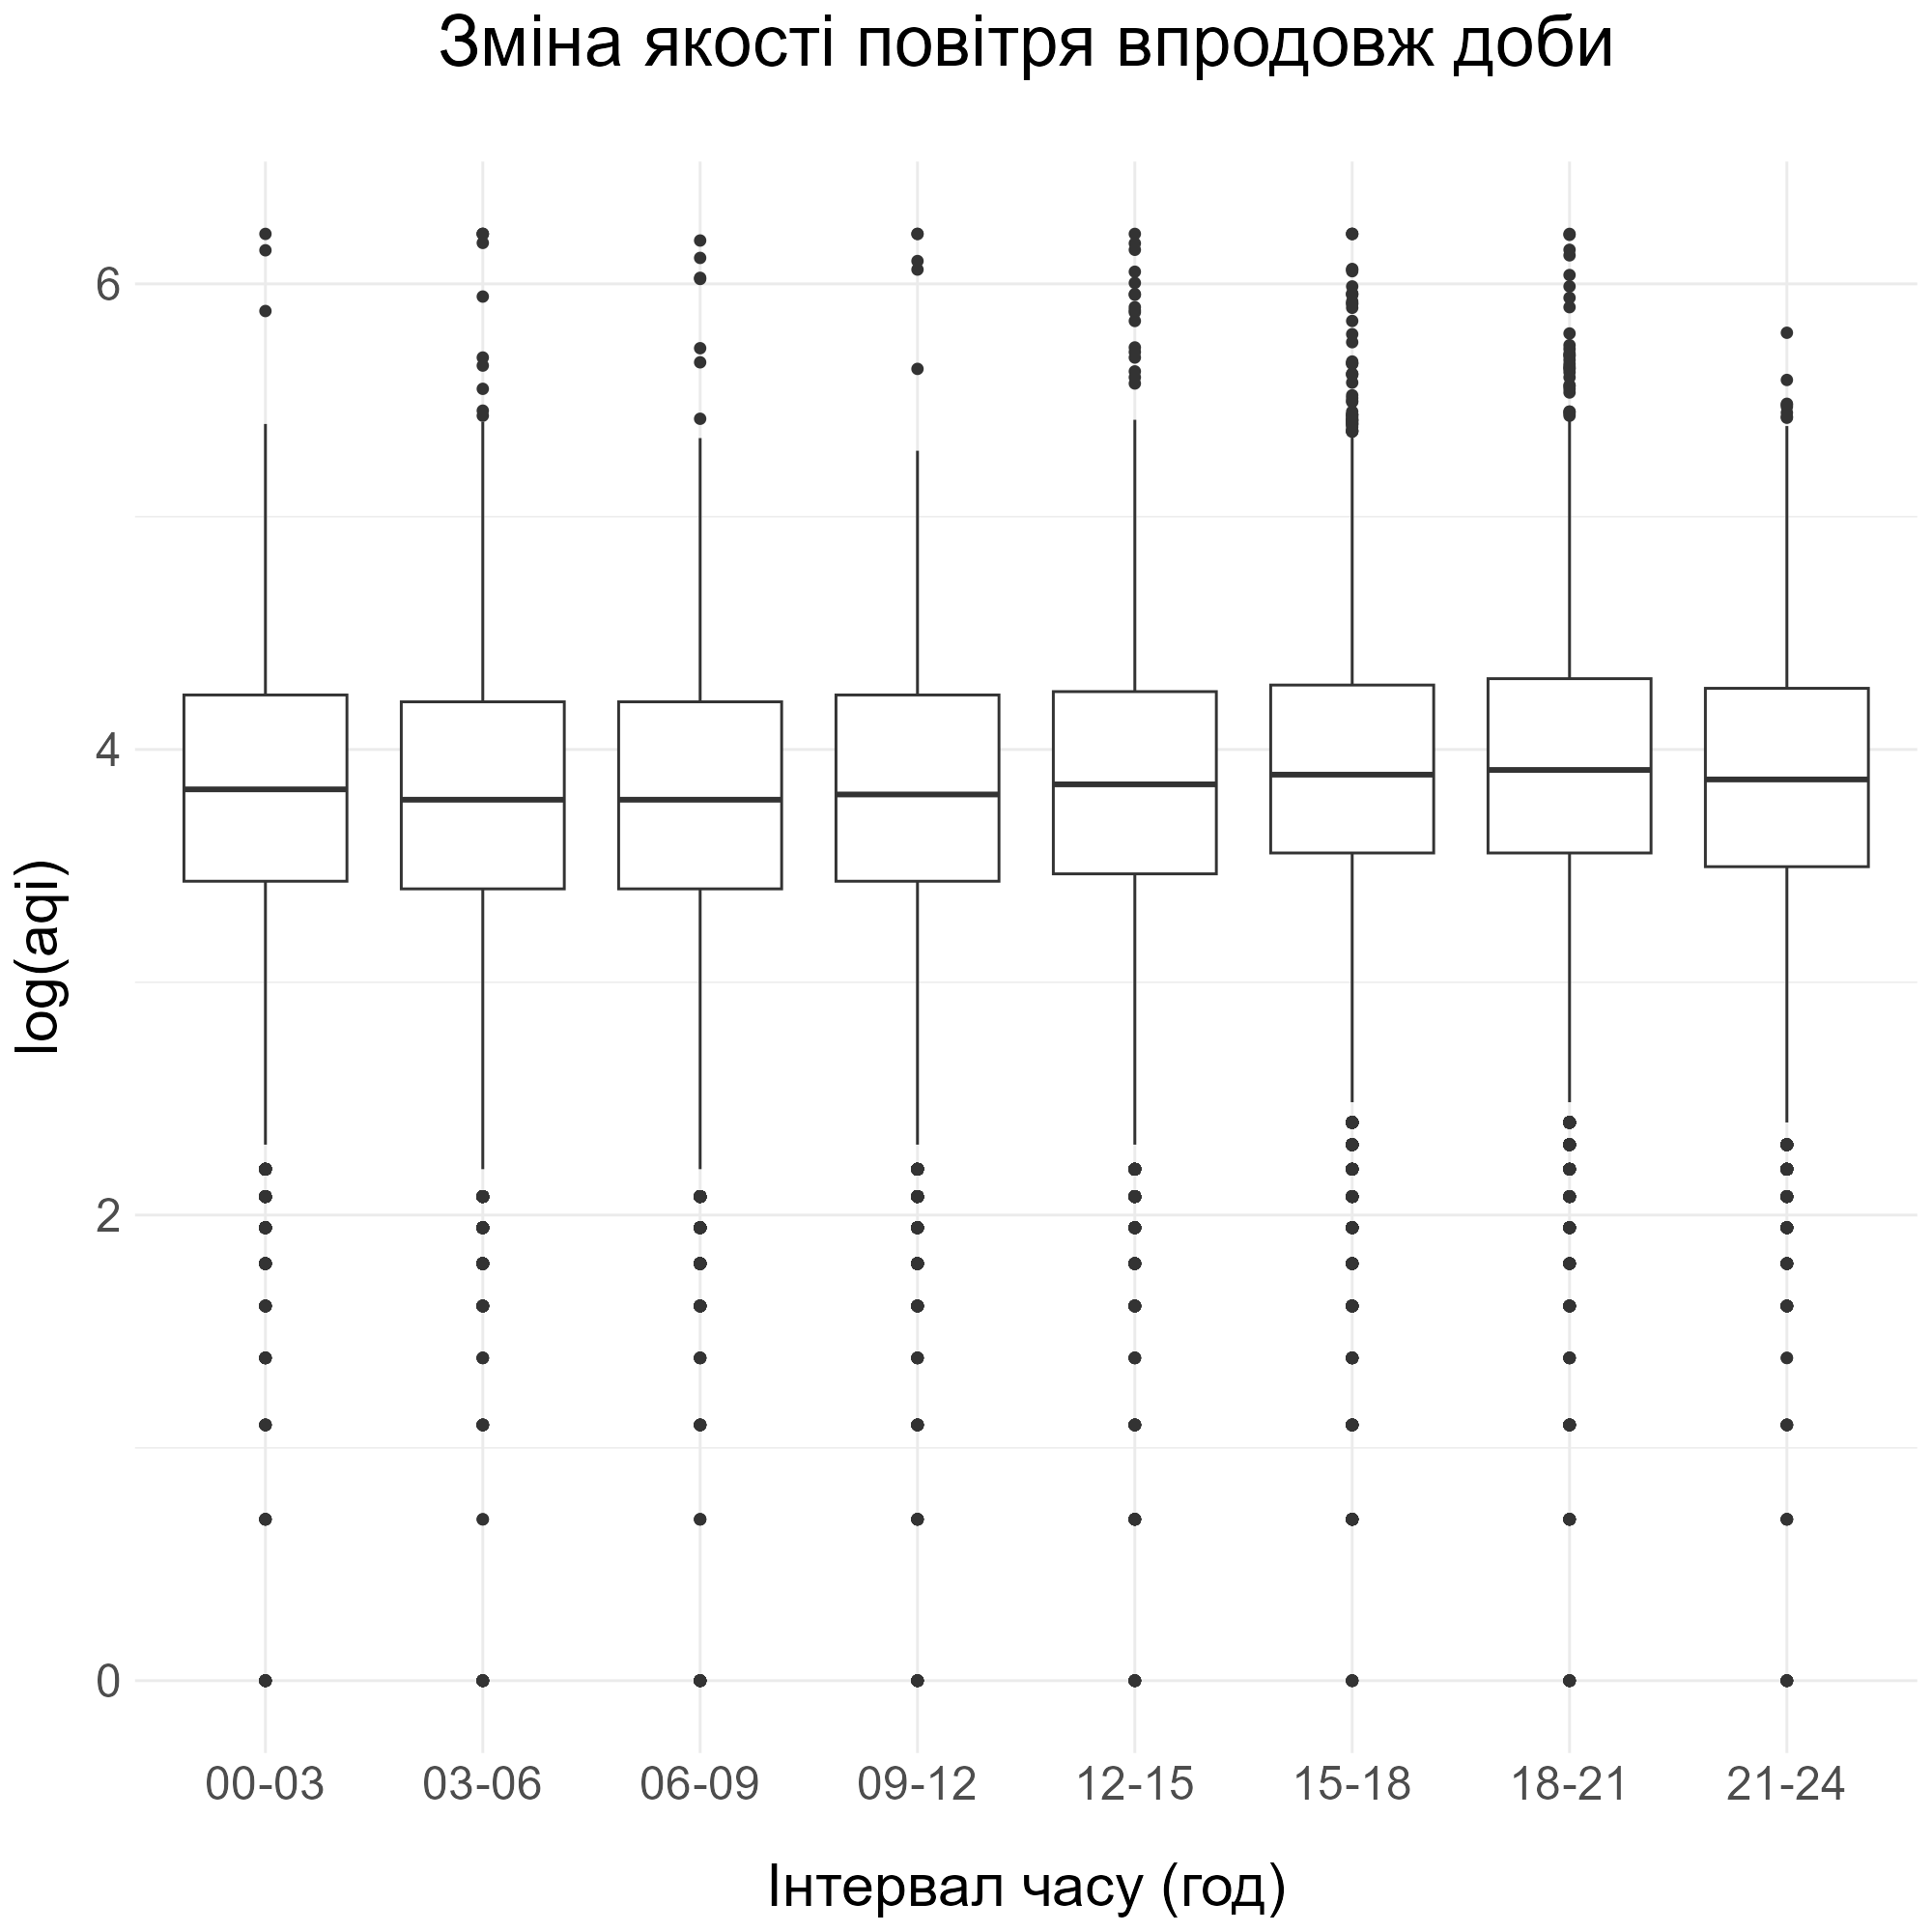
\includegraphics[width=6in]{plots/question3/box.png}
    \end{center}
    Аналізуючи даний графік, можна стверджувтаи,що якість повітря трохи покращується у другій половині дня.
    Також можемо розглянути детальніше регіони та зміни якости повітря. 
    
    \begin{center}
    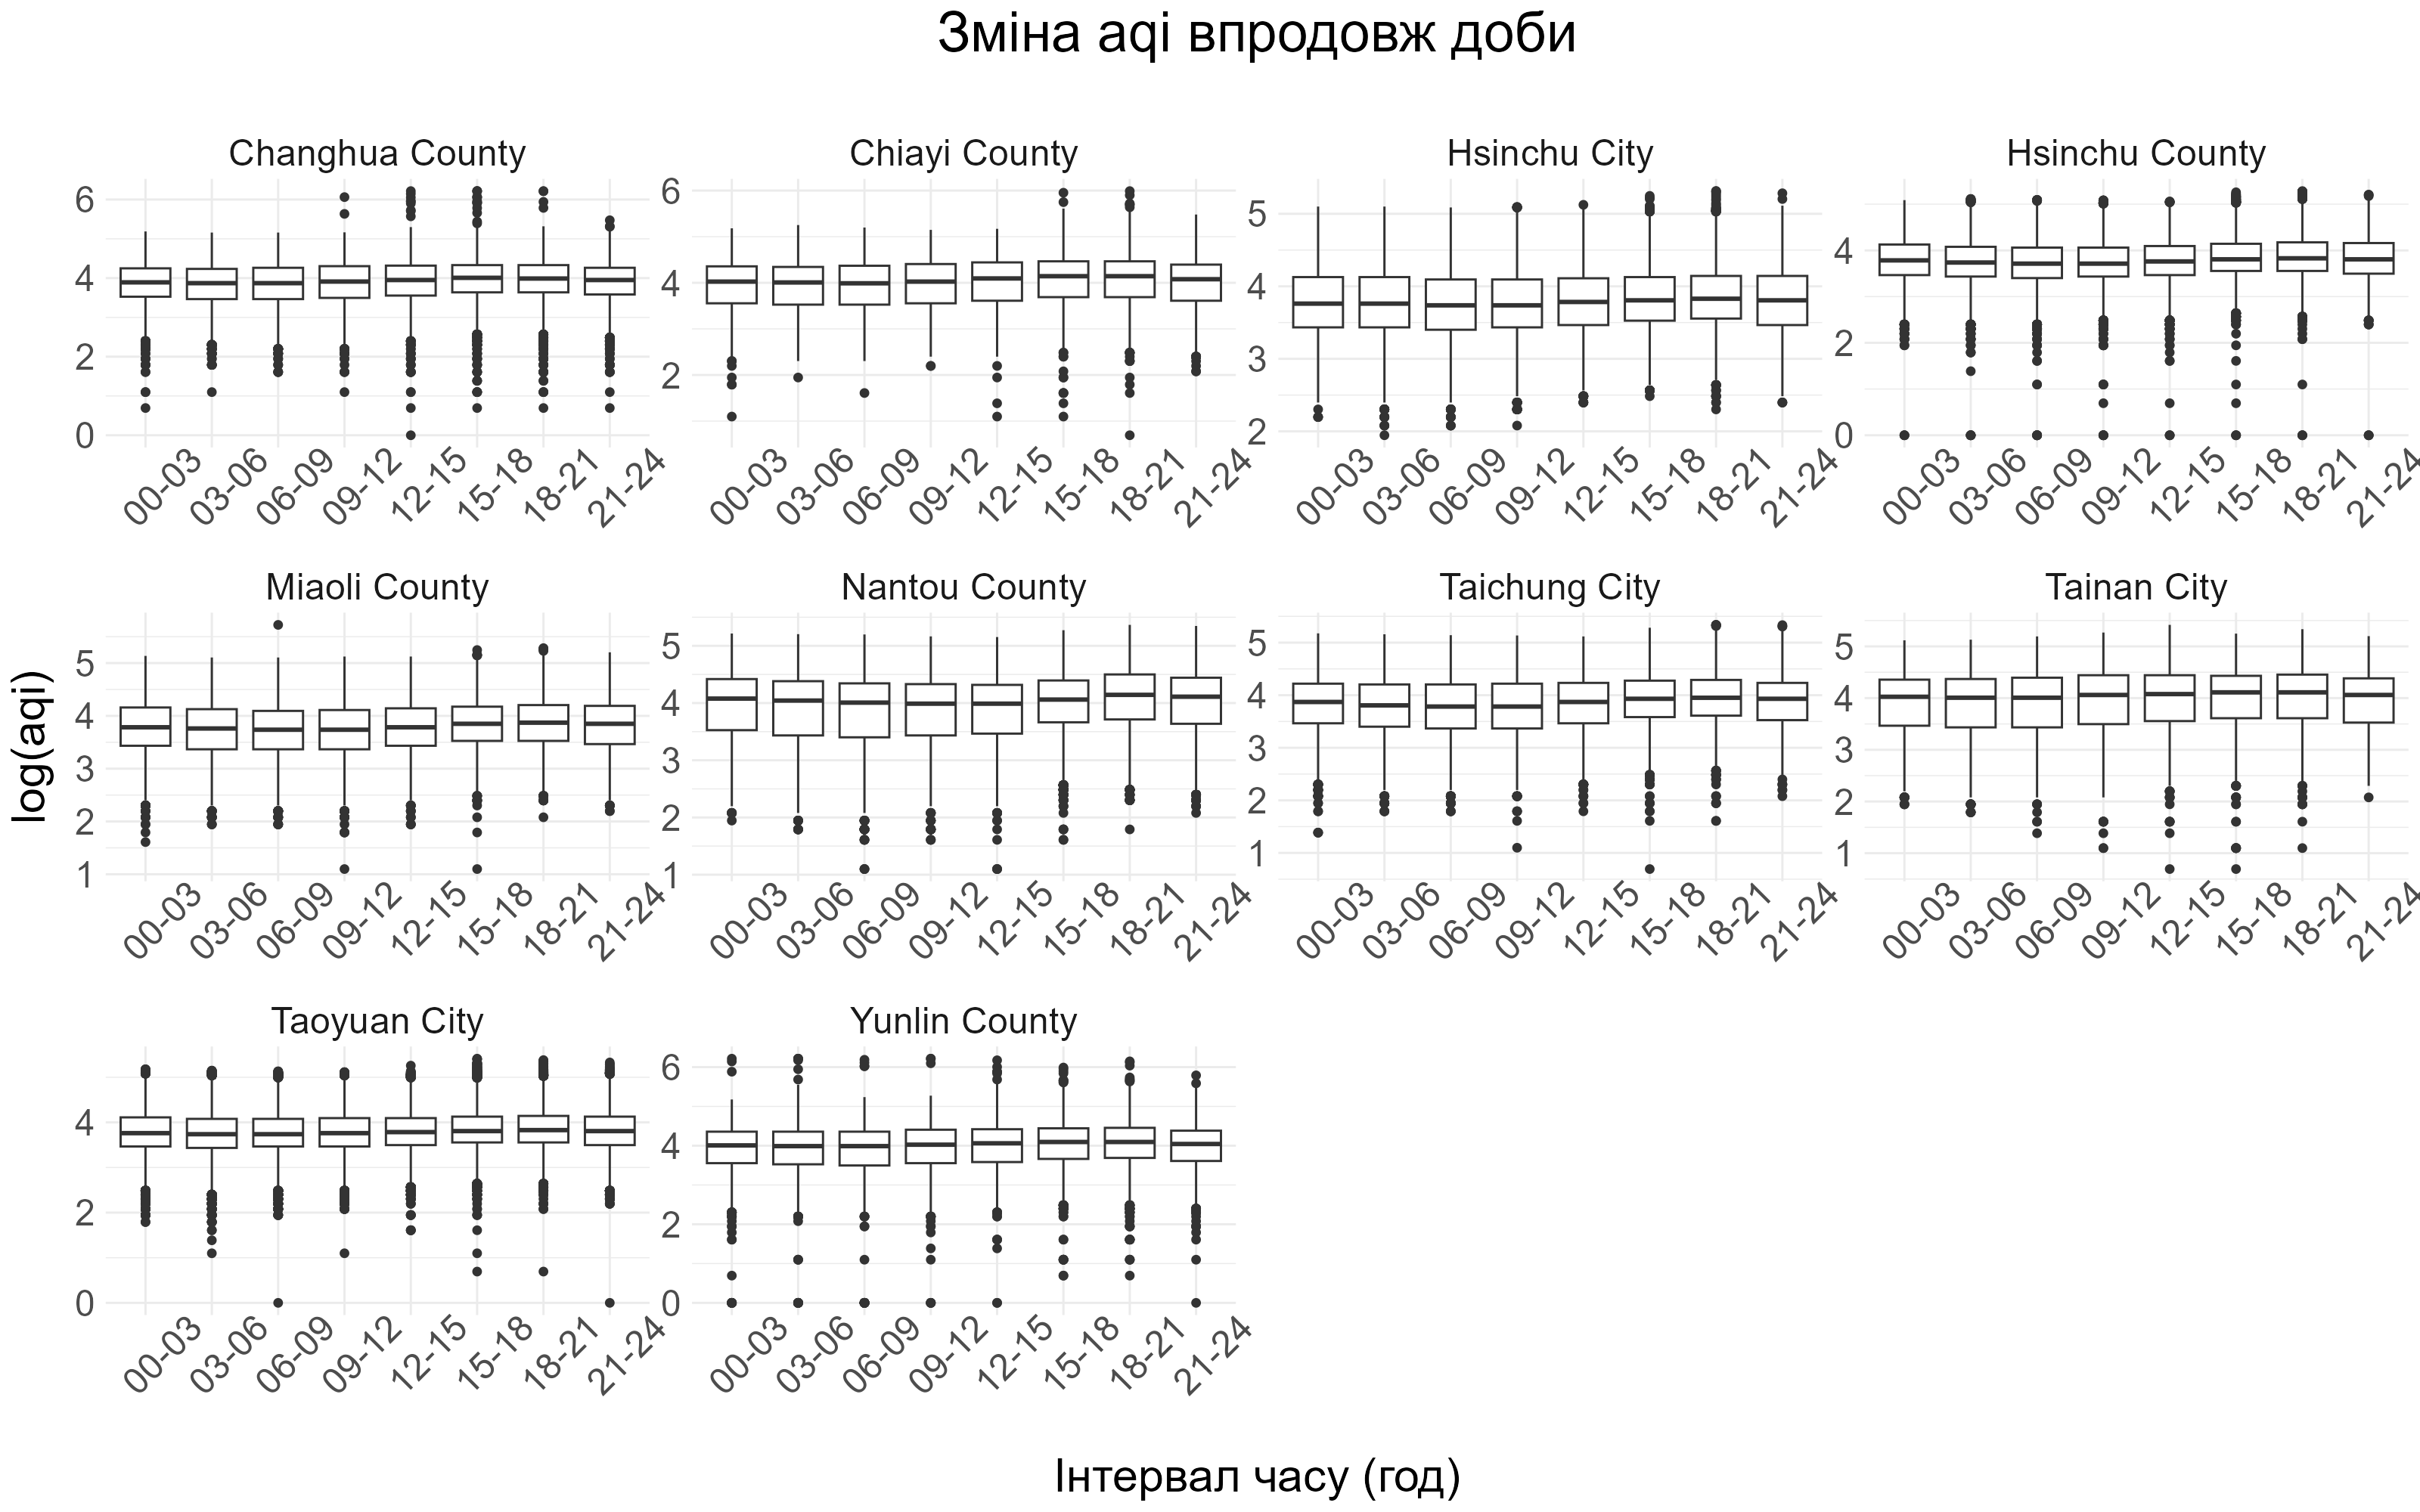
\includegraphics[width=6in]{plots/question3/county-box-p1.png}
    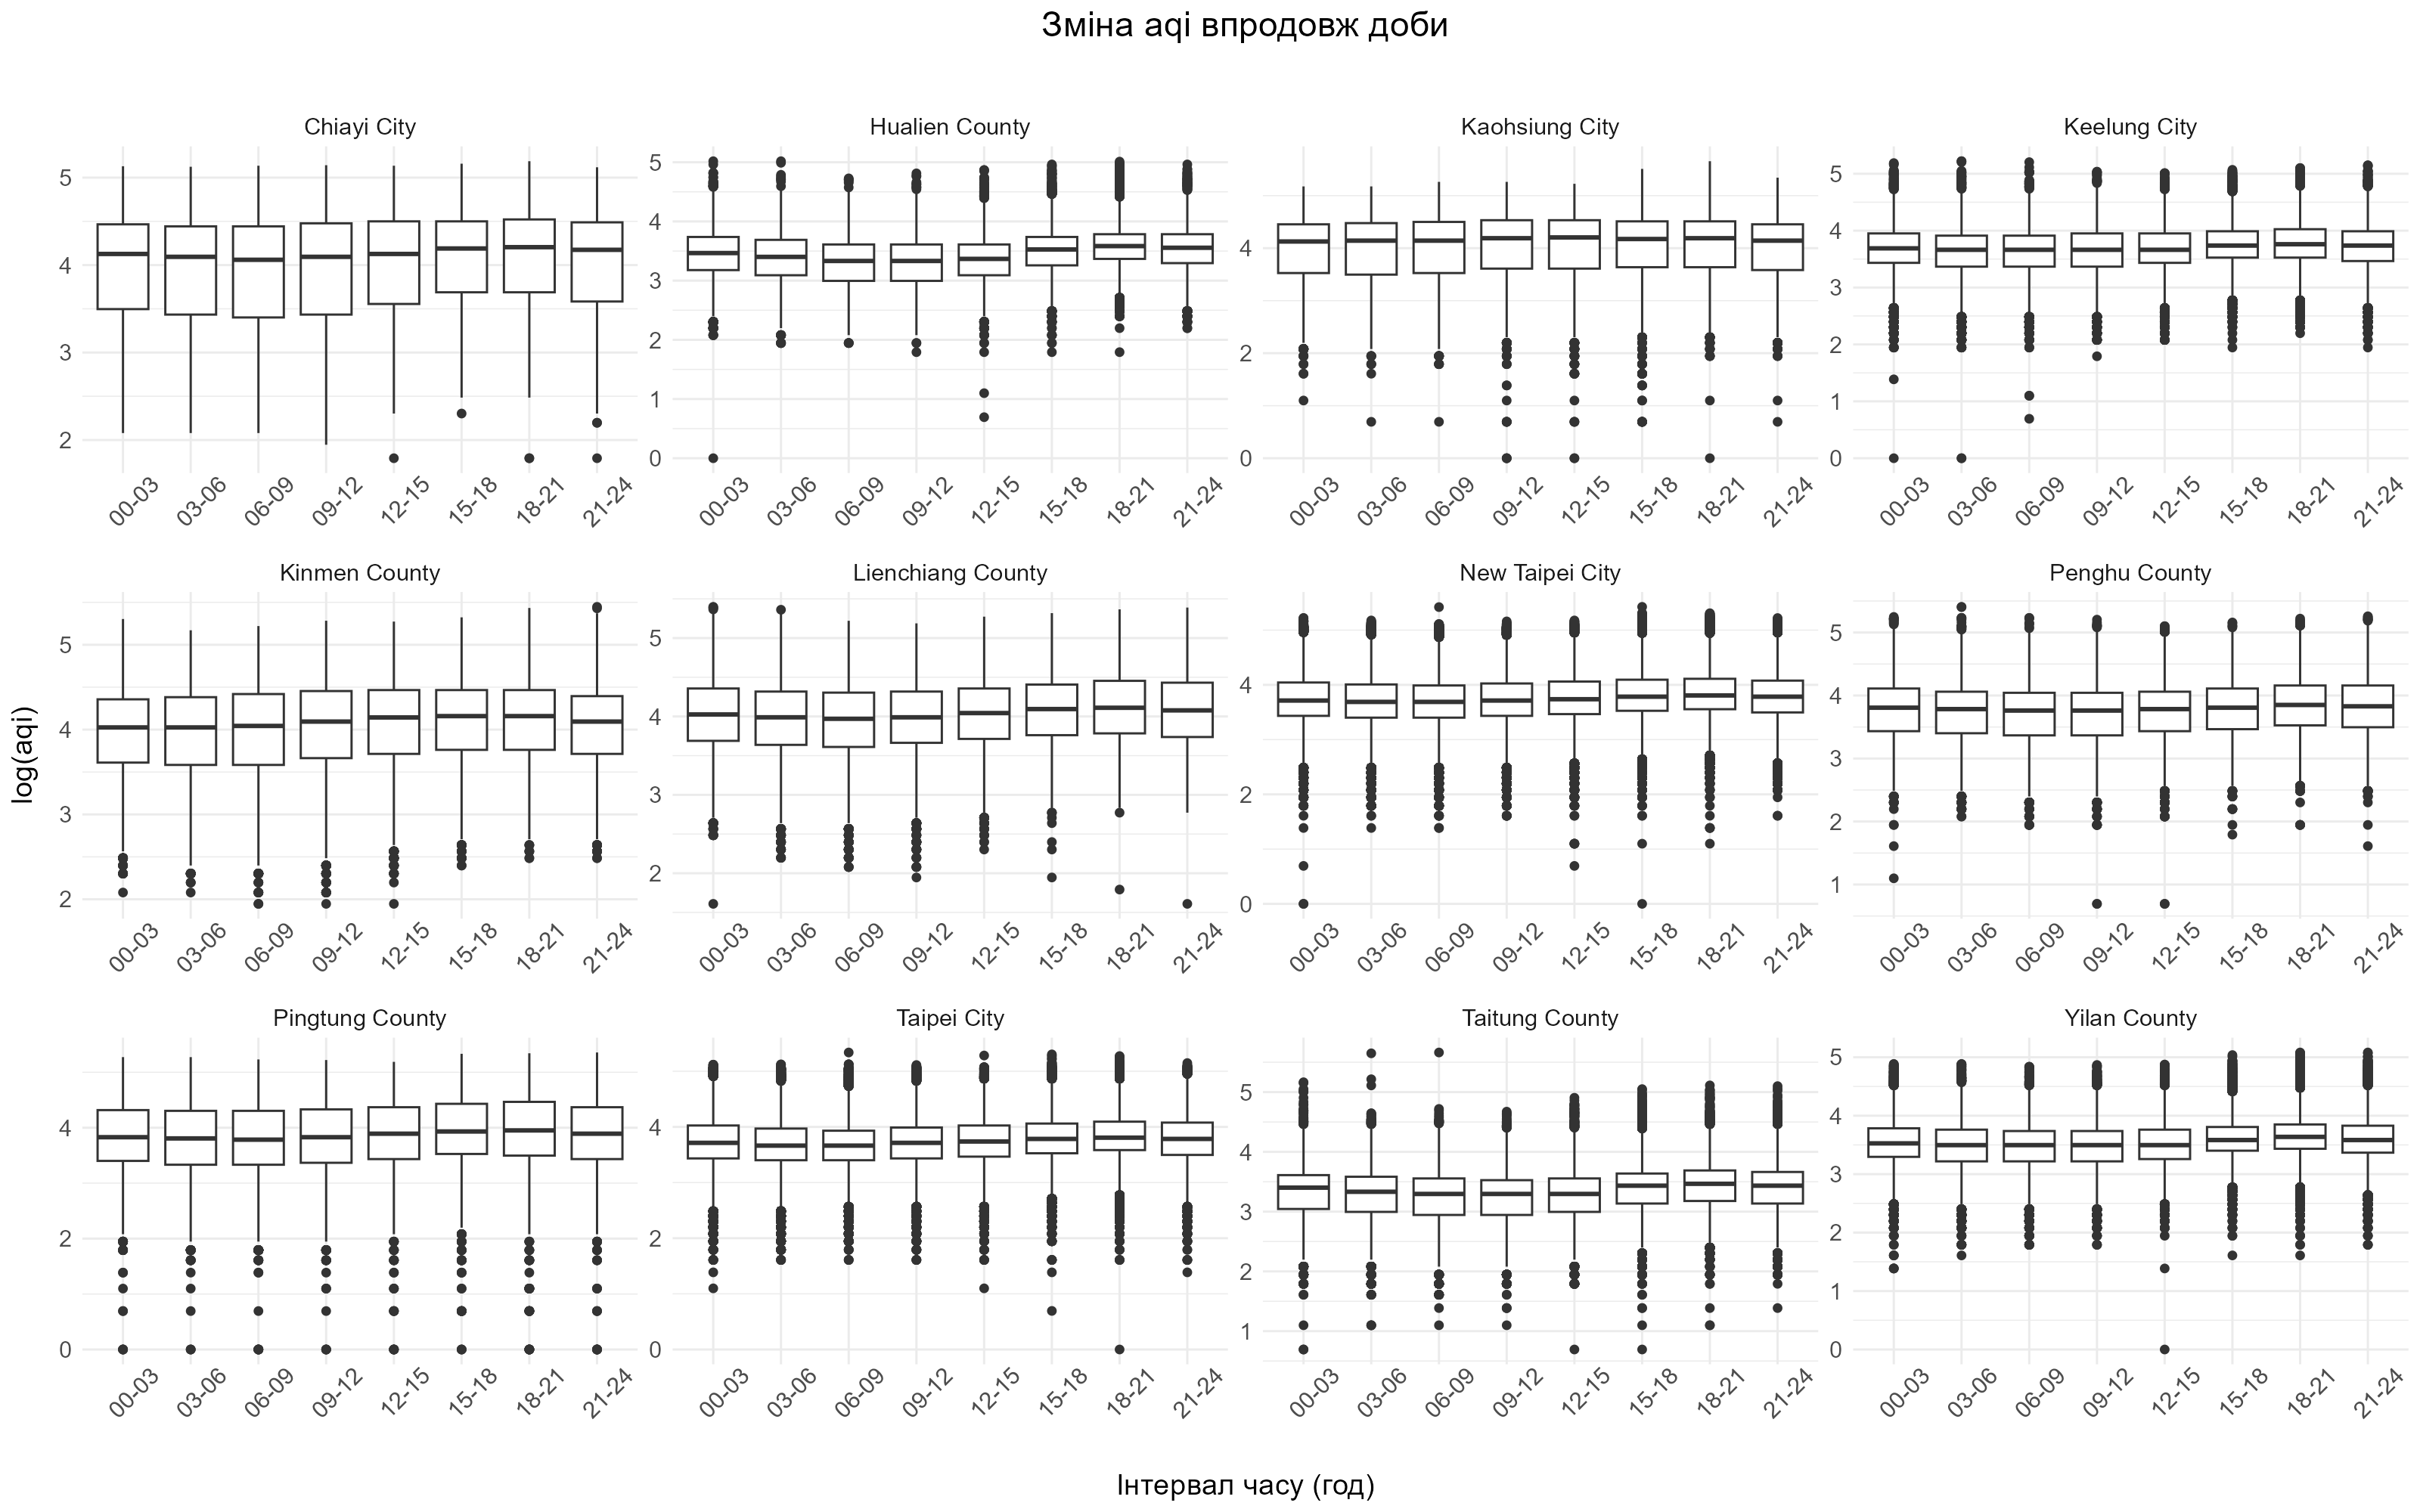
\includegraphics[width=6in]{plots/question3/county-box-p2.png}
    \end{center}

    Бачимо, що проятгом доби по регіонам теж відбуваються незначні зміни  

    \item Які регіони (county) мають найвищий середній рівень забруднення повітря (AQI) протягом року?
    
    \quad \textit{Був використаний trimmed набір даних}

    Всі наступні графіки, будуть будуватися на основі даних за 2016, 2017, 2023 та 2024 роки.
    Для розуміння числових даних, розглянемо 10 регіонів з найвищим рівнем AQI за відповідні роки.
 
    \begin{table}
        \centering
        \begin{minipage}{0.45\textwidth}
            \centering
            \begin{tabular}{ccc}
                \textbf{Year} & \textbf{County} & \textbf{avg\_AQI} \\
                \toprule
                2016 & Chiayi City & 120.31 \\
                2016 & Kaohsiung City & 112.10 \\
                2016 & Tainan City & 99.60 \\
                2016 & Pingtung County & 97.15 \\
                2016 & Yunlin County & 91.23 \\
                2016 & Chiayi County & 88.83 \\
                2016 & Nantou County & 83.34 \\
                2016 & Changhua County & 81.68 \\
                2016 & Kinmen County & 81.60 \\
                2016 & Taichung City & 77.96 \\
                \midrule
            \end{tabular}
            \caption{Середнє AQI за 2016}
        \end{minipage}
        \hspace{0.05\textwidth} % Додає відстань між таблицями
        \begin{minipage}{0.45\textwidth}
            \centering
            \begin{tabular}{ccc}
                \textbf{Year} & \textbf{County} & \textbf{avg\_AQI} \\
                \toprule
                2017 & Kinmen County & 79.77 \\
                2017 & Kaohsiung City & 79.31 \\
                2017 & Yunlin County & 77.24 \\
                2017 & Nantou County & 76.42 \\
                2017 & Tainan City & 74.00 \\
                2017 & Chiayi County & 73.40 \\
                2017 & Changhua County & 72.39 \\
                2017 & Chiayi City & 71.89 \\
                2017 & Pingtung County & 70.10 \\
                2017 & Lienchiang County & 66.44 \\
                \midrule
            \end{tabular}
            \caption{Середнє AQI за 2017}
        \end{minipage}
    \end{table}
    
    \begin{table}
        \centering
        \begin{minipage}{0.45\textwidth}
            \centering
            \begin{tabular}{ccc}
                \textbf{Year} & \textbf{County} & \textbf{avg\_AQI} \\
                \toprule
                2023&	Kinmen County	   &64.90551\\	
                2023&	Lienchiang County  &61.09091\\	
                2023&	Chiayi City	       &60.36290\\	
                2023&	Chiayi County	   &59.45318\\	
                2023&	Kaohsiung City	   &59.29308\\	
                2023&	Tainan City	       &56.54597\\	
                2023&	Yunlin County	   &54.93570\\	
                2023&	Changhua County	   &54.02576\\	
                2023&	Nantou County	   &52.30822\\	
                2023&	Pingtung County	   &50.73770\\
                \midrule
            \end{tabular}
            \caption{Середнє AQI за 2016}
        \end{minipage}
        \hspace{0.05\textwidth} % Додає відстань між таблицями
        \begin{minipage}{0.45\textwidth}
            \centering
            \begin{tabular}{ccc}
                \textbf{Year} & \textbf{County} & \textbf{avg\_AQI} \\
                \toprule
                2024&	Kinmen County	   &66.82609	\\	
                2024&	Lienchiang County  &58.25882	\\	
                2024&	Chiayi County	   &55.87912	\\	
                2024&	Chiayi City	       &55.83784	\\	
                2024&	Yunlin County	   &54.74169	\\	
                2024&	Kaohsiung City	   &54.05860	\\	
                2024&	Tainan City	       &53.17339	\\	
                2024&	Nantou County	   &51.36140	\\	
                2024&	Changhua County	   &51.12869	\\	
                2024&	Taichung City	   &49.87937	\\
                \midrule
            \end{tabular}
            \caption{Середнє AQI за 2017}
        \end{minipage}
    \end{table}
    
    Візуалізуючи чітко можна відмітити найбільш забруднені регіони.
    \begin{center}
    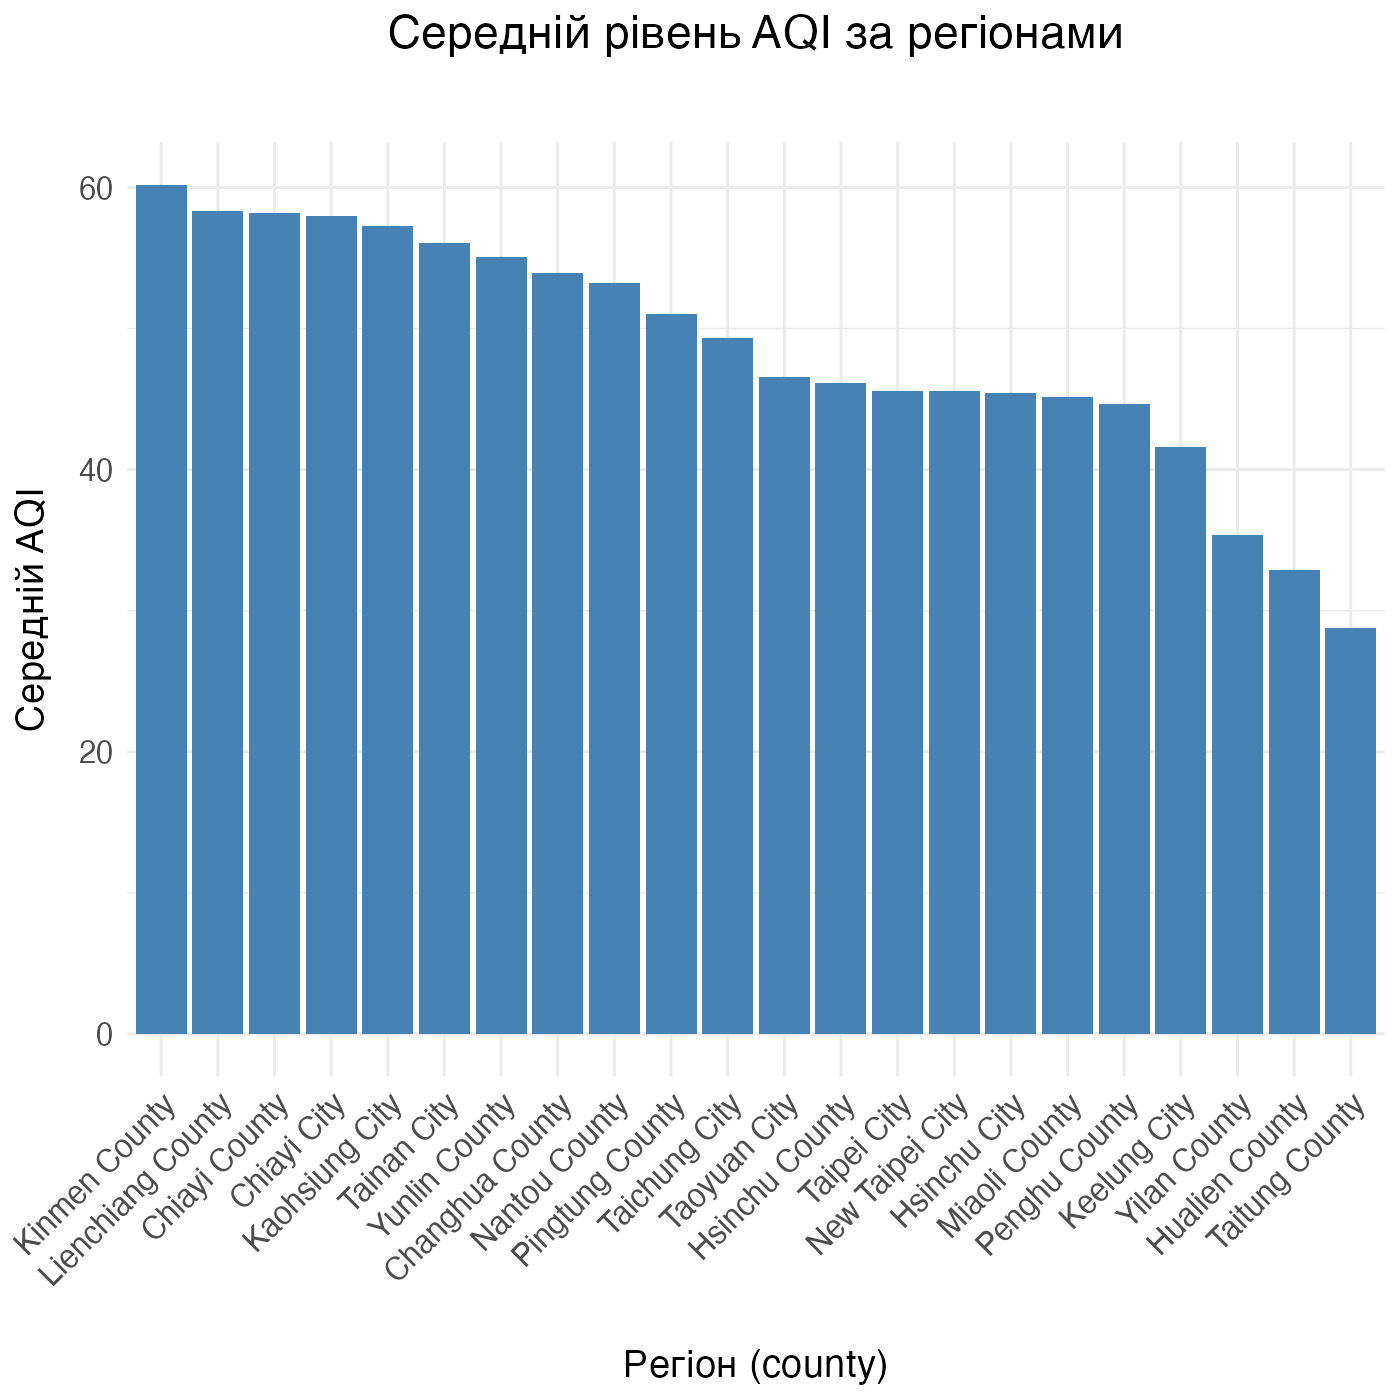
\includegraphics[width=6in]{plots/question4/avg_aqi_by_county.png}
    \end{center}

    Також можемо порівняти якість повітря в залежності від щільності населення. Проте це не дає однознанчої відповіді чи повязані ці значення між собою.
    \begin{center}
    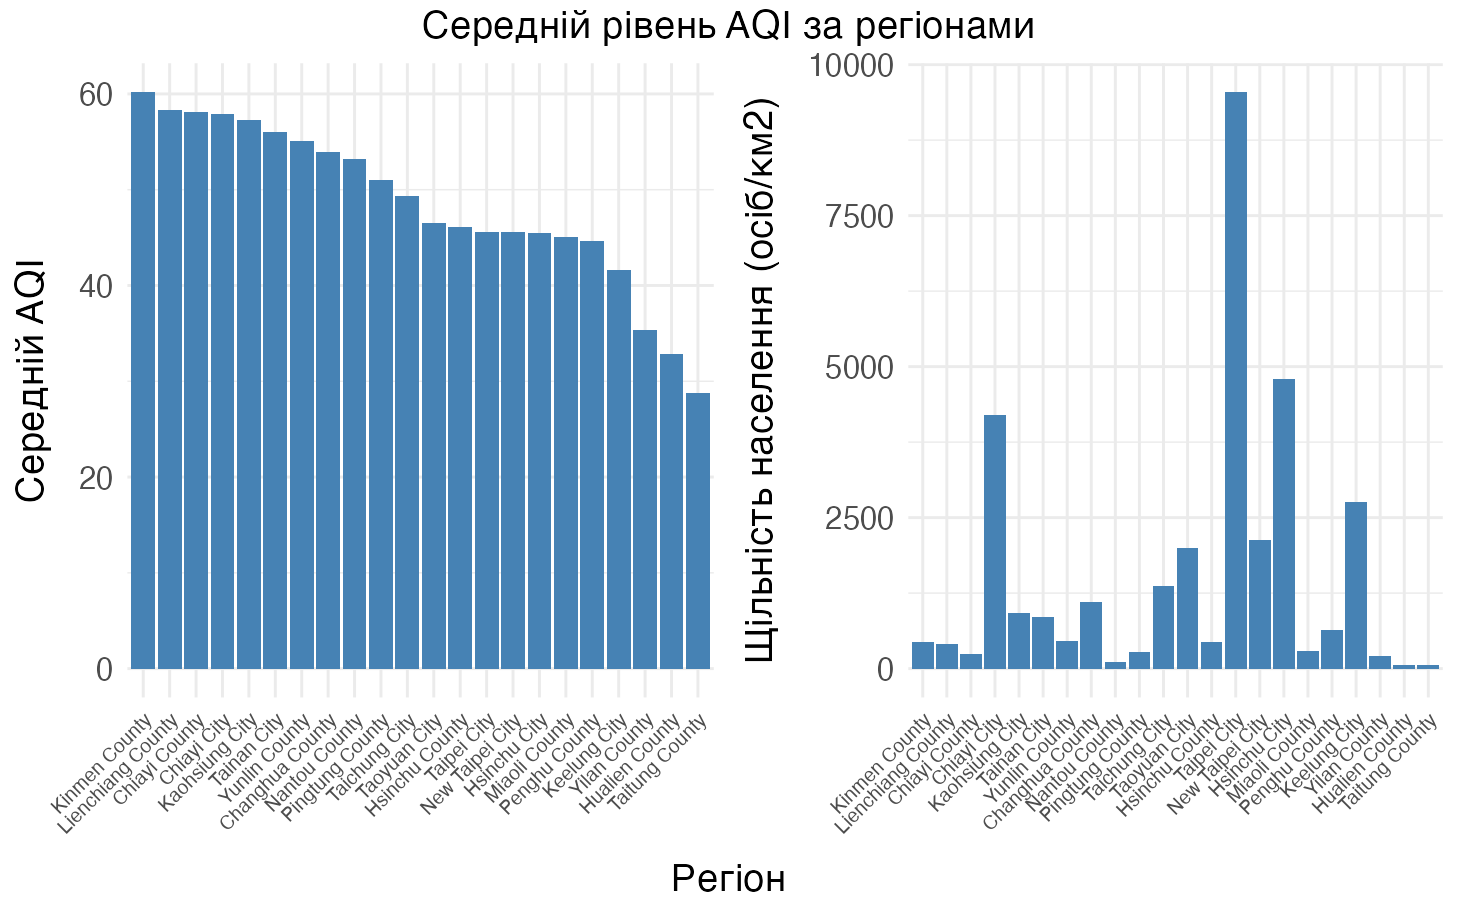
\includegraphics[width=6in]{plots/question4/avg_aqi_by_county_w_dens.png}
    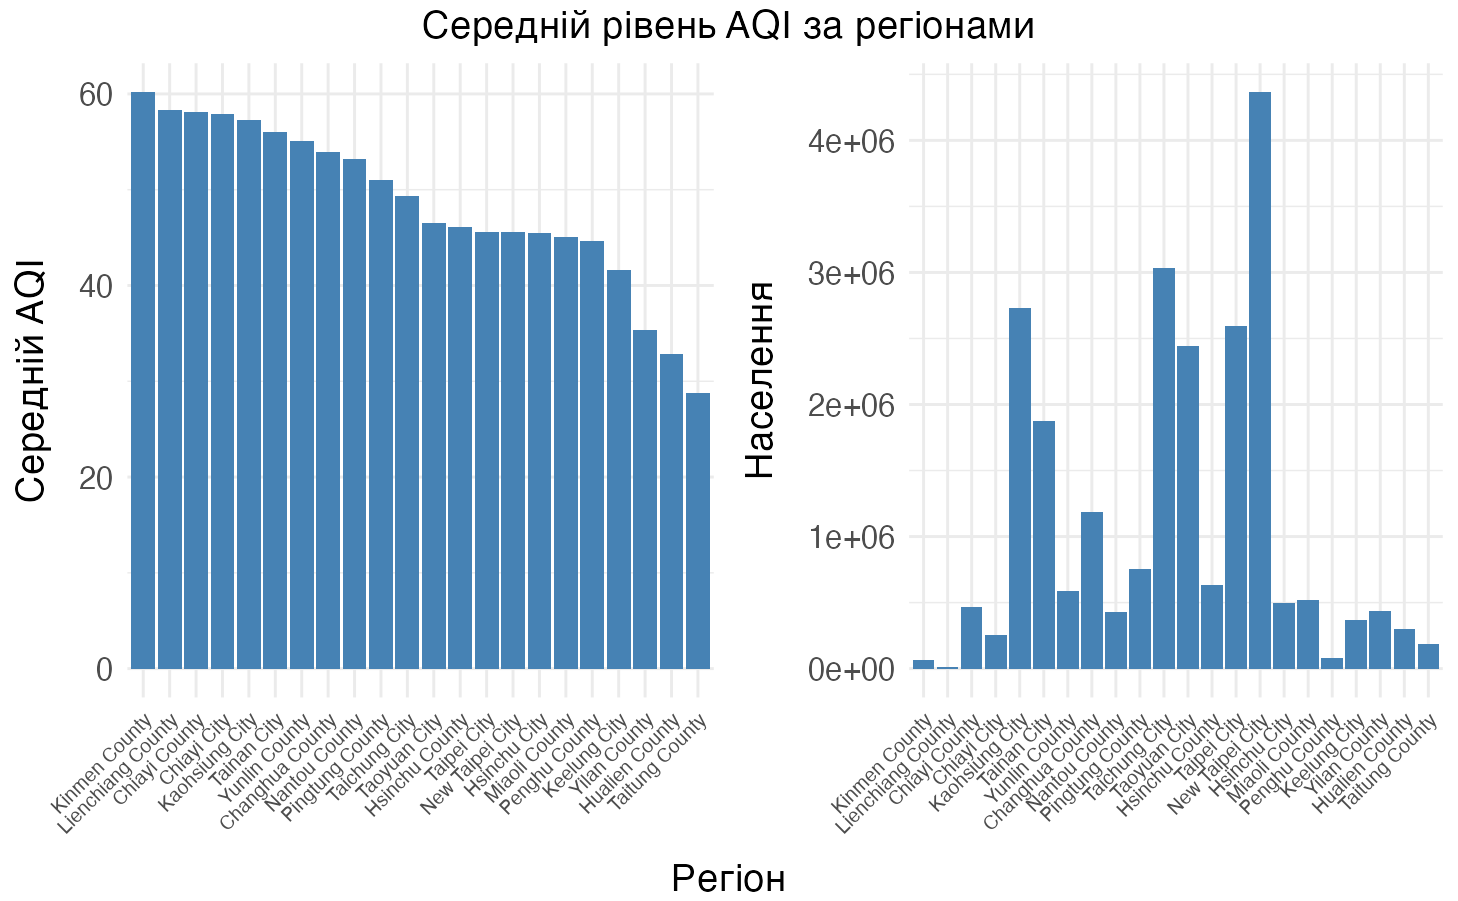
\includegraphics[width=6in]{plots/question4/avg_aqi_by_county_w_pop.png}
    \end{center}

    Якщо розглядати рівень якости повітря по сезонно, то можна відмітити, що влітку показники явно кращі, ніж в холодні пори року. Це може бути спричинено погодиними умовами, такі як сезони дощі, часті пориви вітру та інше.
    
    \begin{center}
    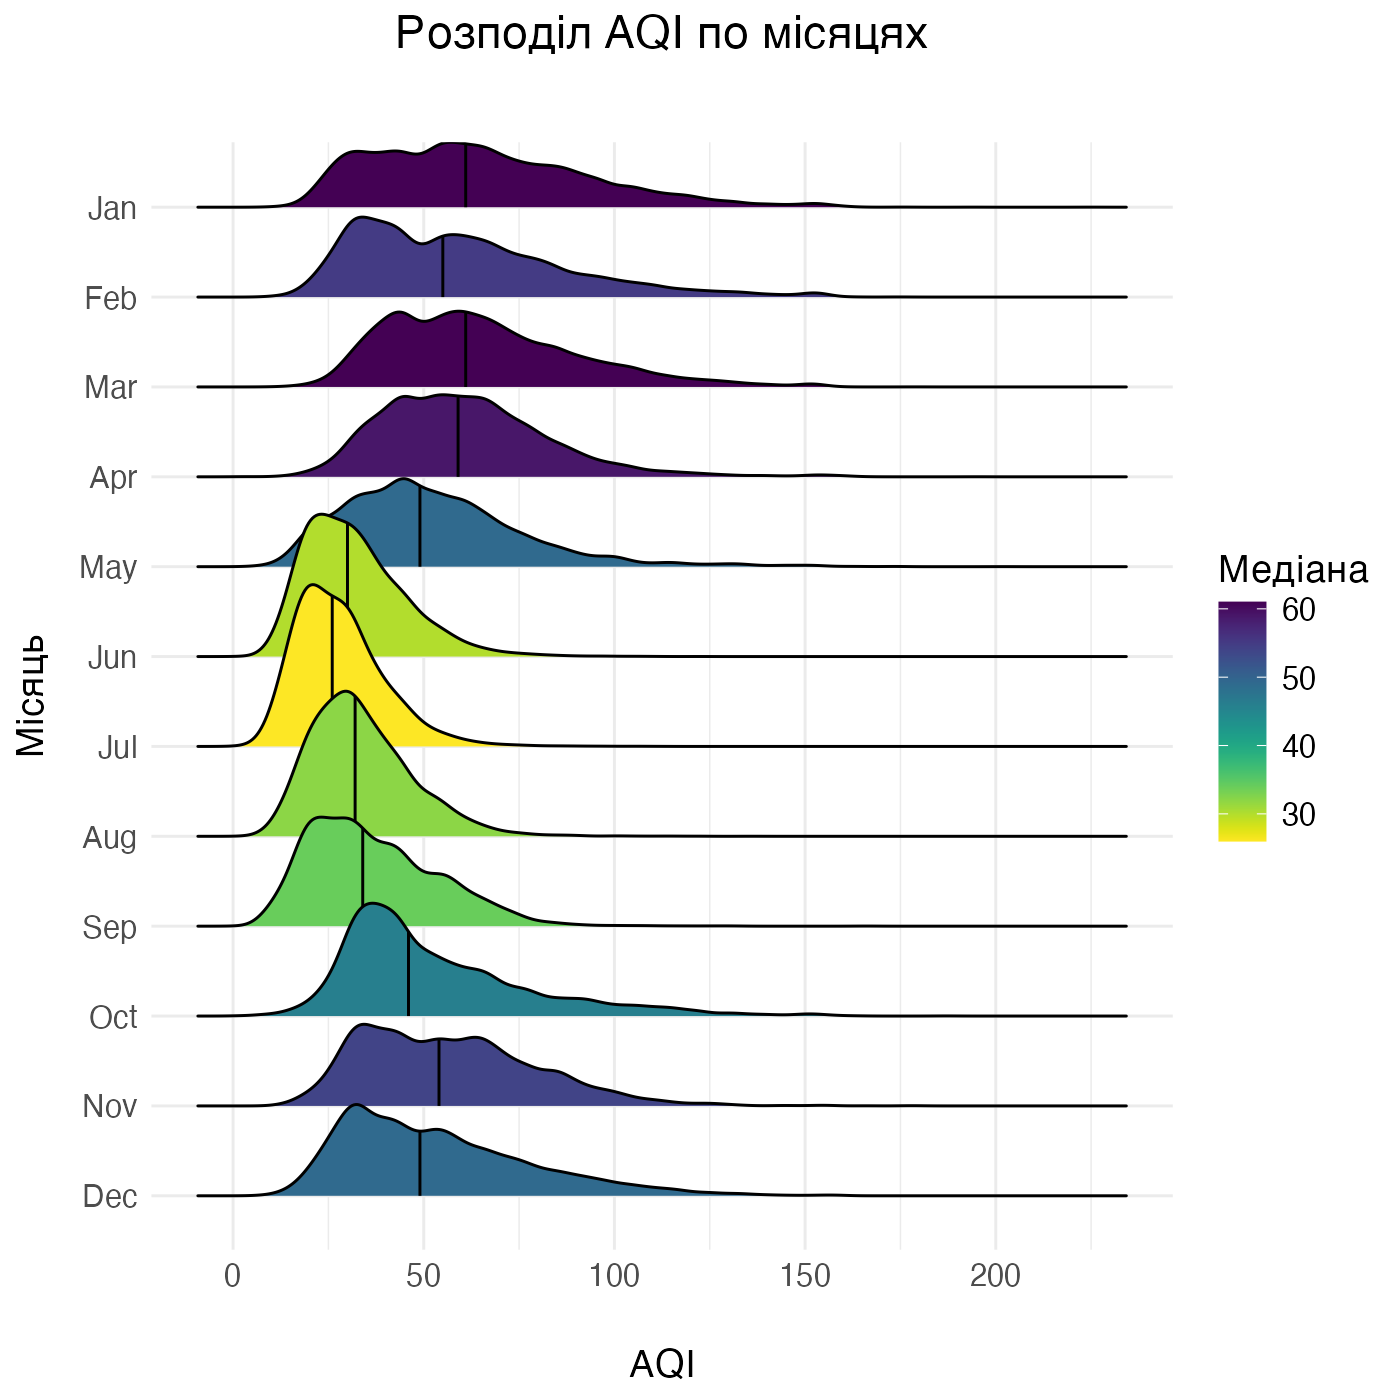
\includegraphics[width=6in]{plots/question4/seasonal_change_ridgeline.png}
    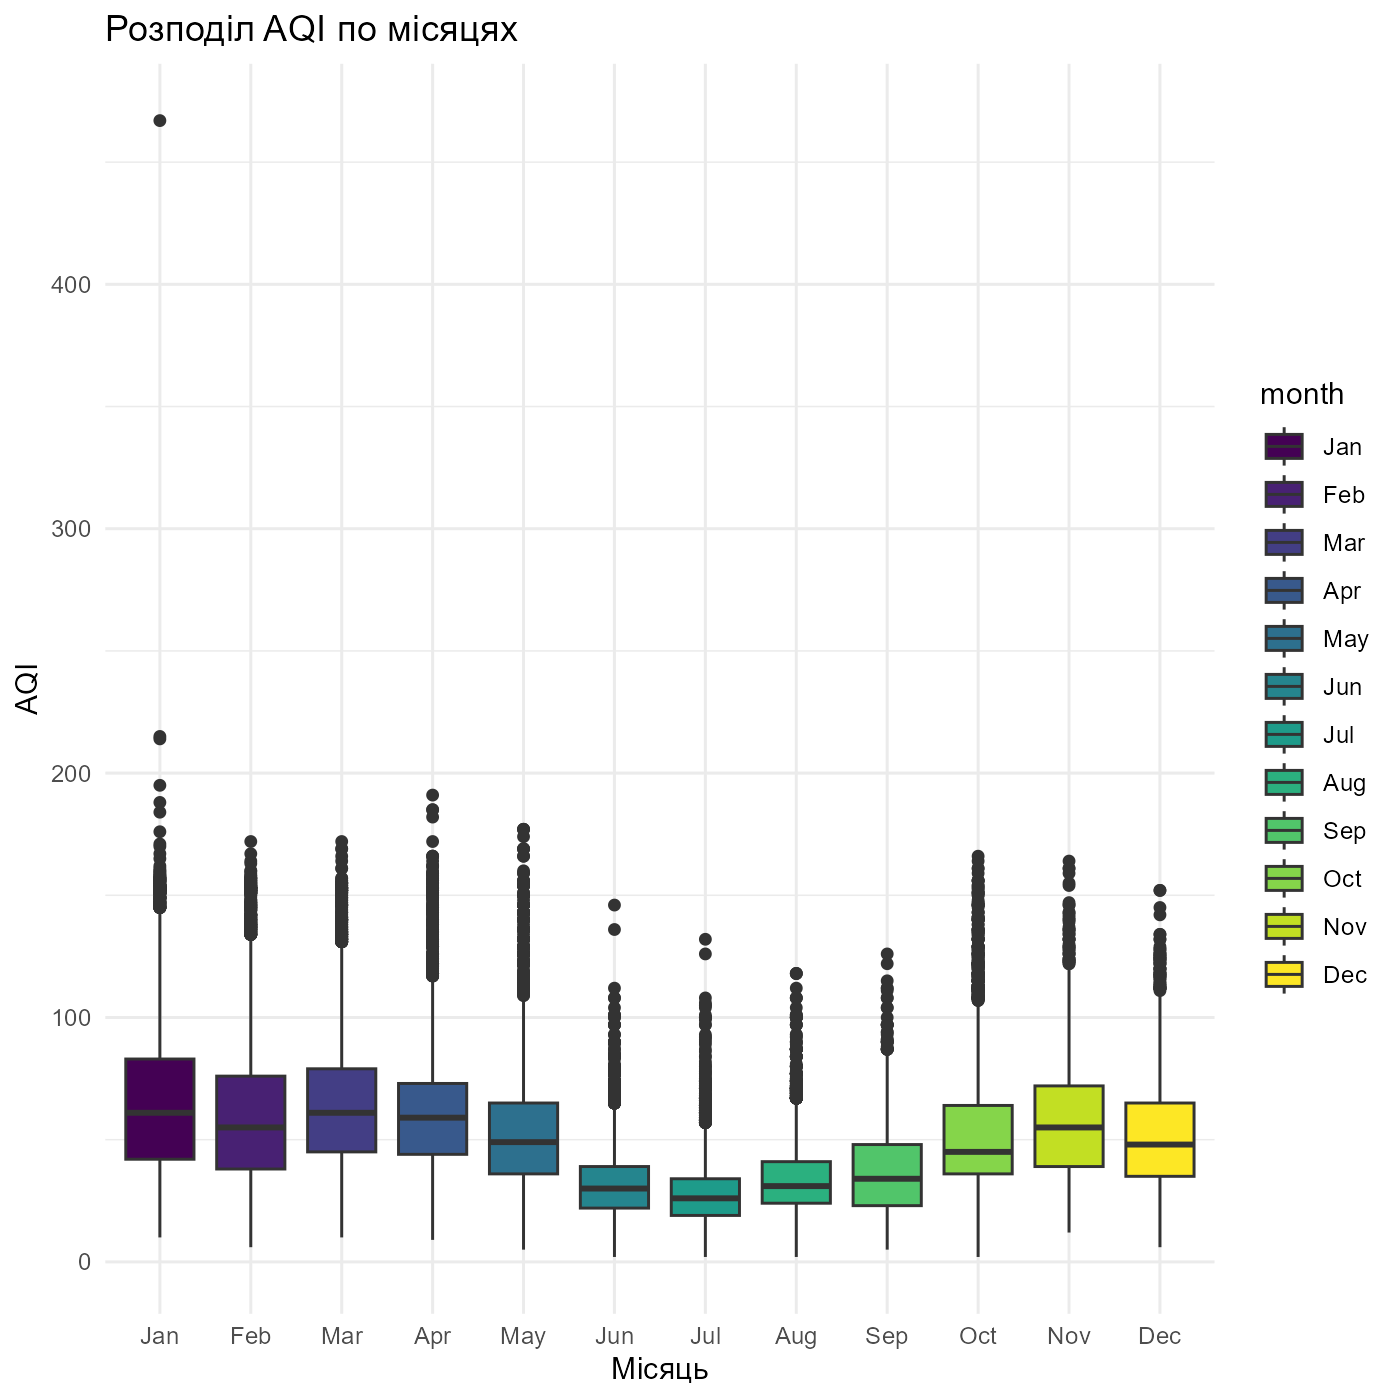
\includegraphics[width=6in]{plots/question4/seasonal_change.png}
    \end{center} 

    \item Як змінився загальний рівень забруднення по регіонам після початку реформи?
    
    \quad \textit{Був використаний tidy набір даних}

    Для загального кількісного розуміння можна переглянути таблиці з результатми середнього значення в попередньому питанні. 
    Далі візуалізуємо середнє значення якости повітря за 5 місяців від початку вимірювання показників і до початку реформи. Відповідно так само візуалізуємо за останні 5 місців вже під час реформи. 
    Задля розуміння рівня по всій країні, обрано графік map. 
    
    \begin{center}
    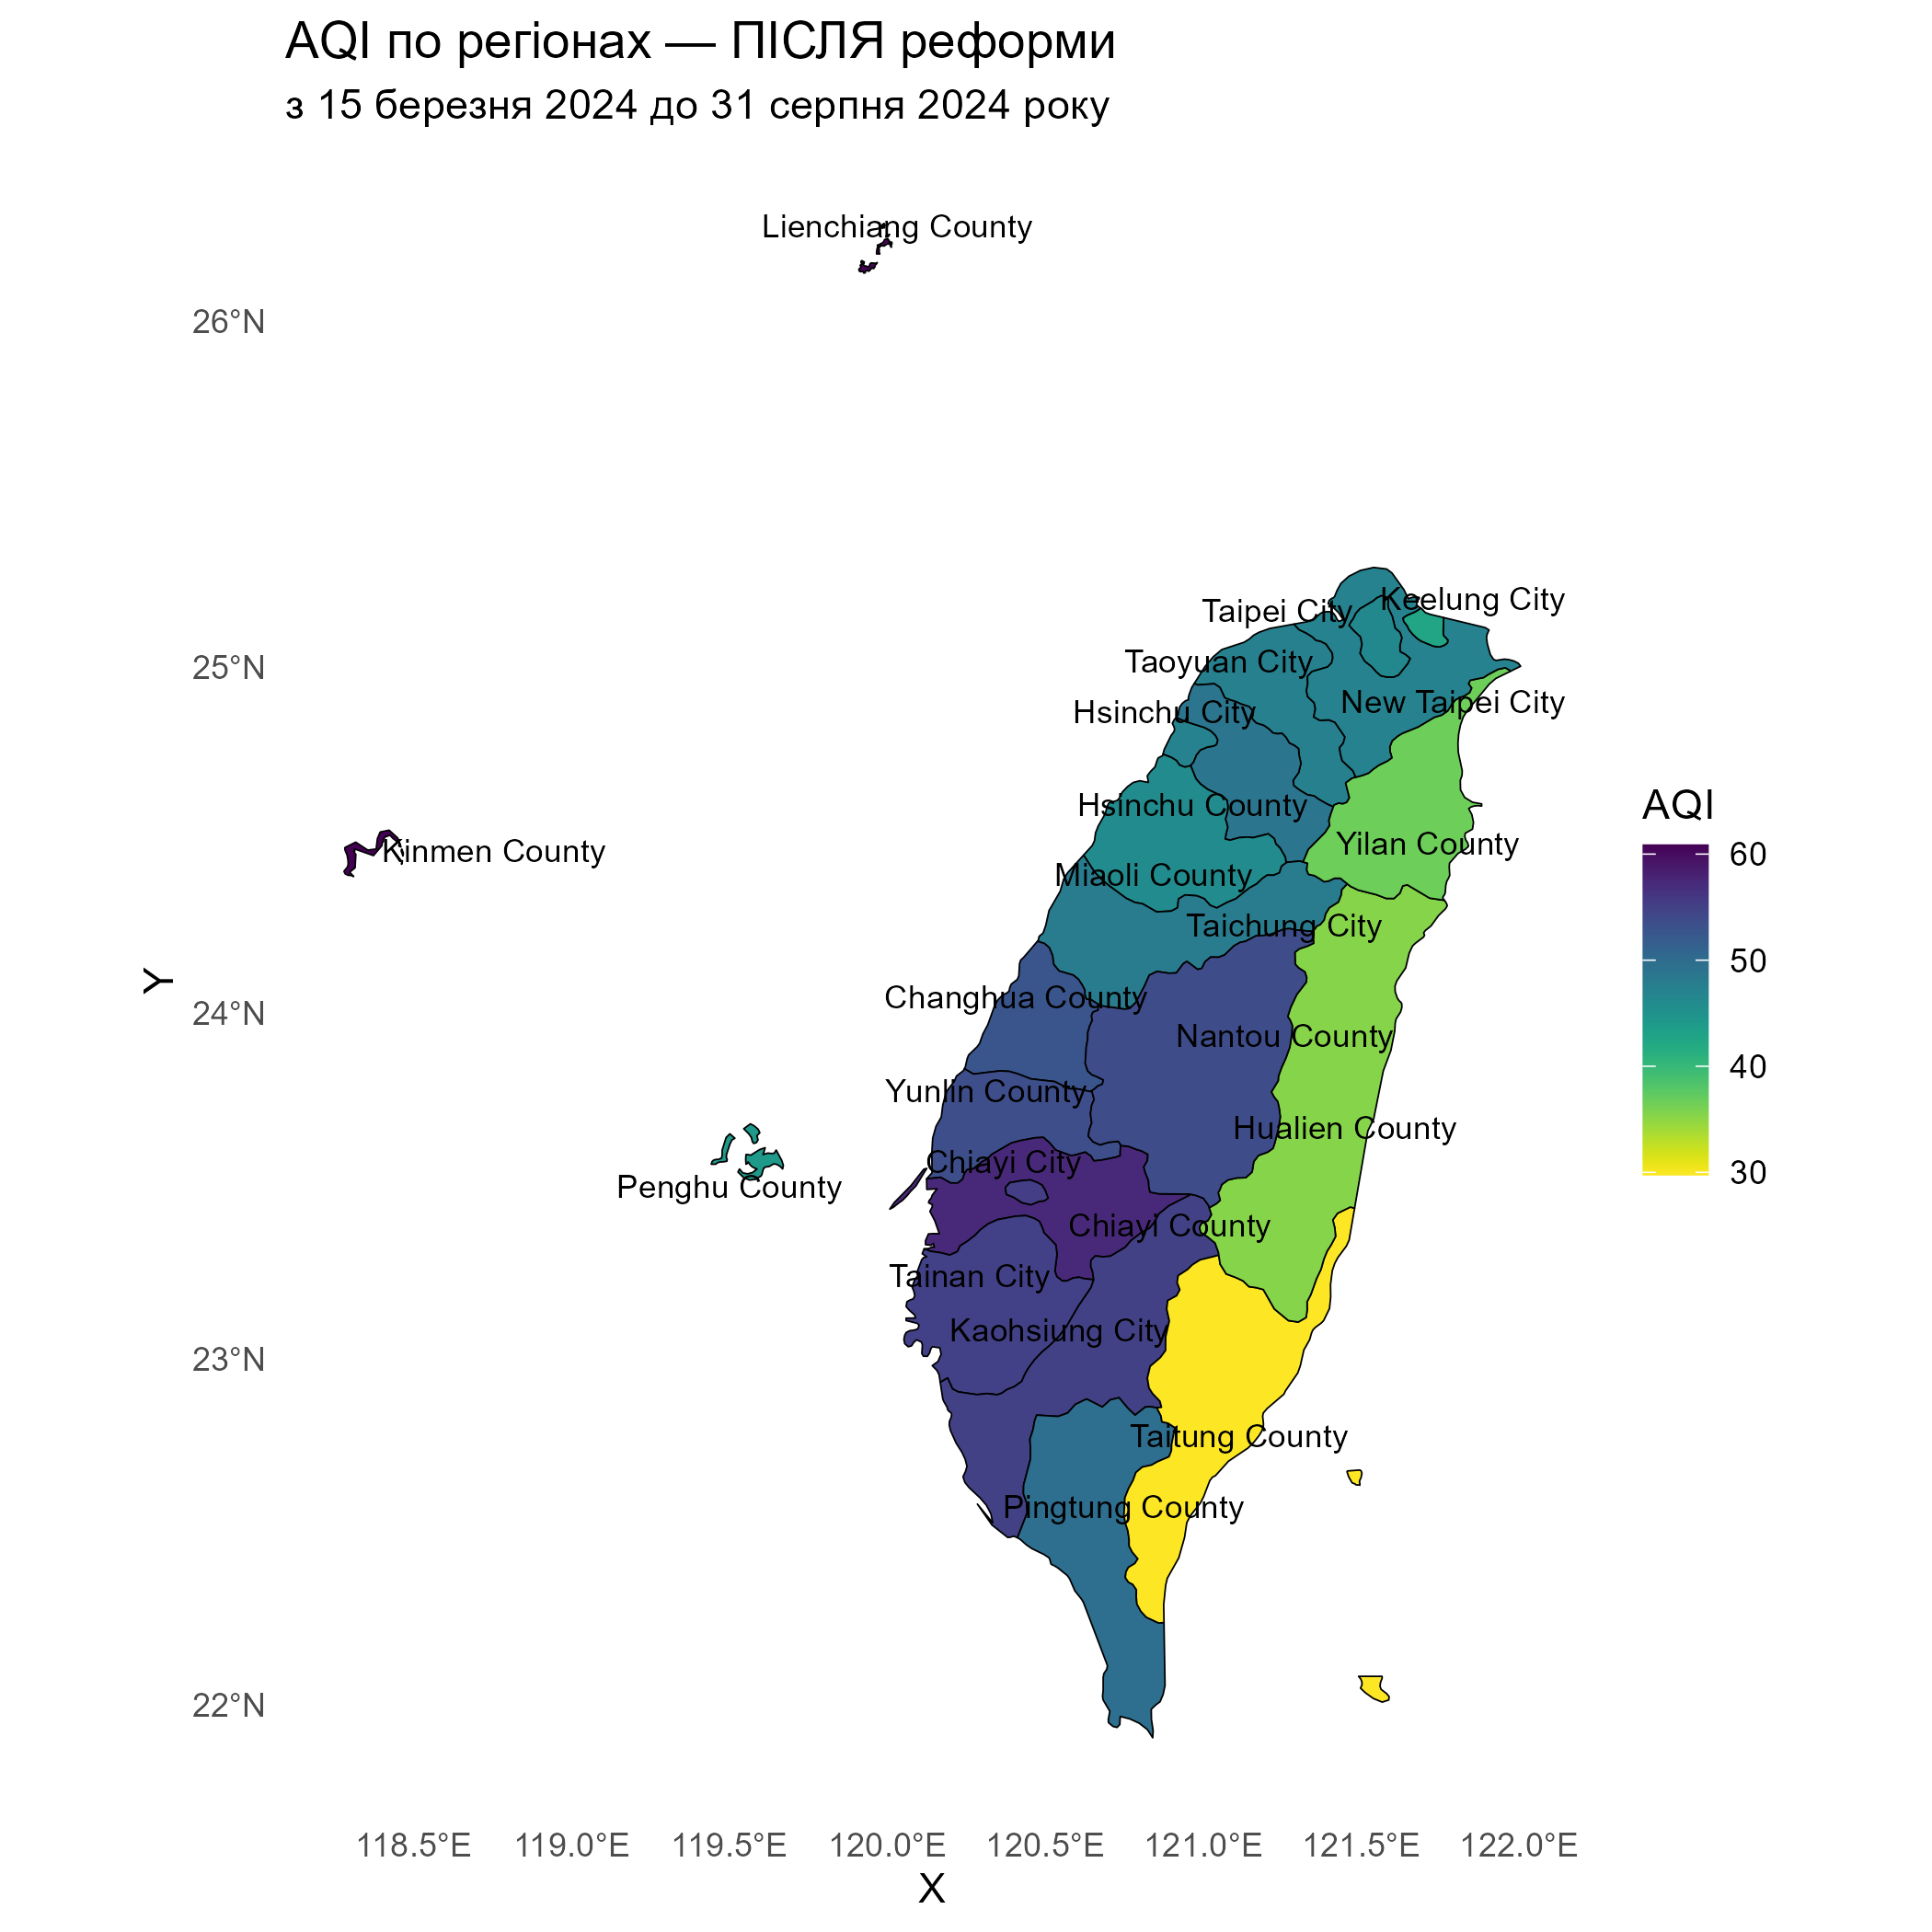
\includegraphics[width=6in]{plots/question5/map_after_reform.png}
    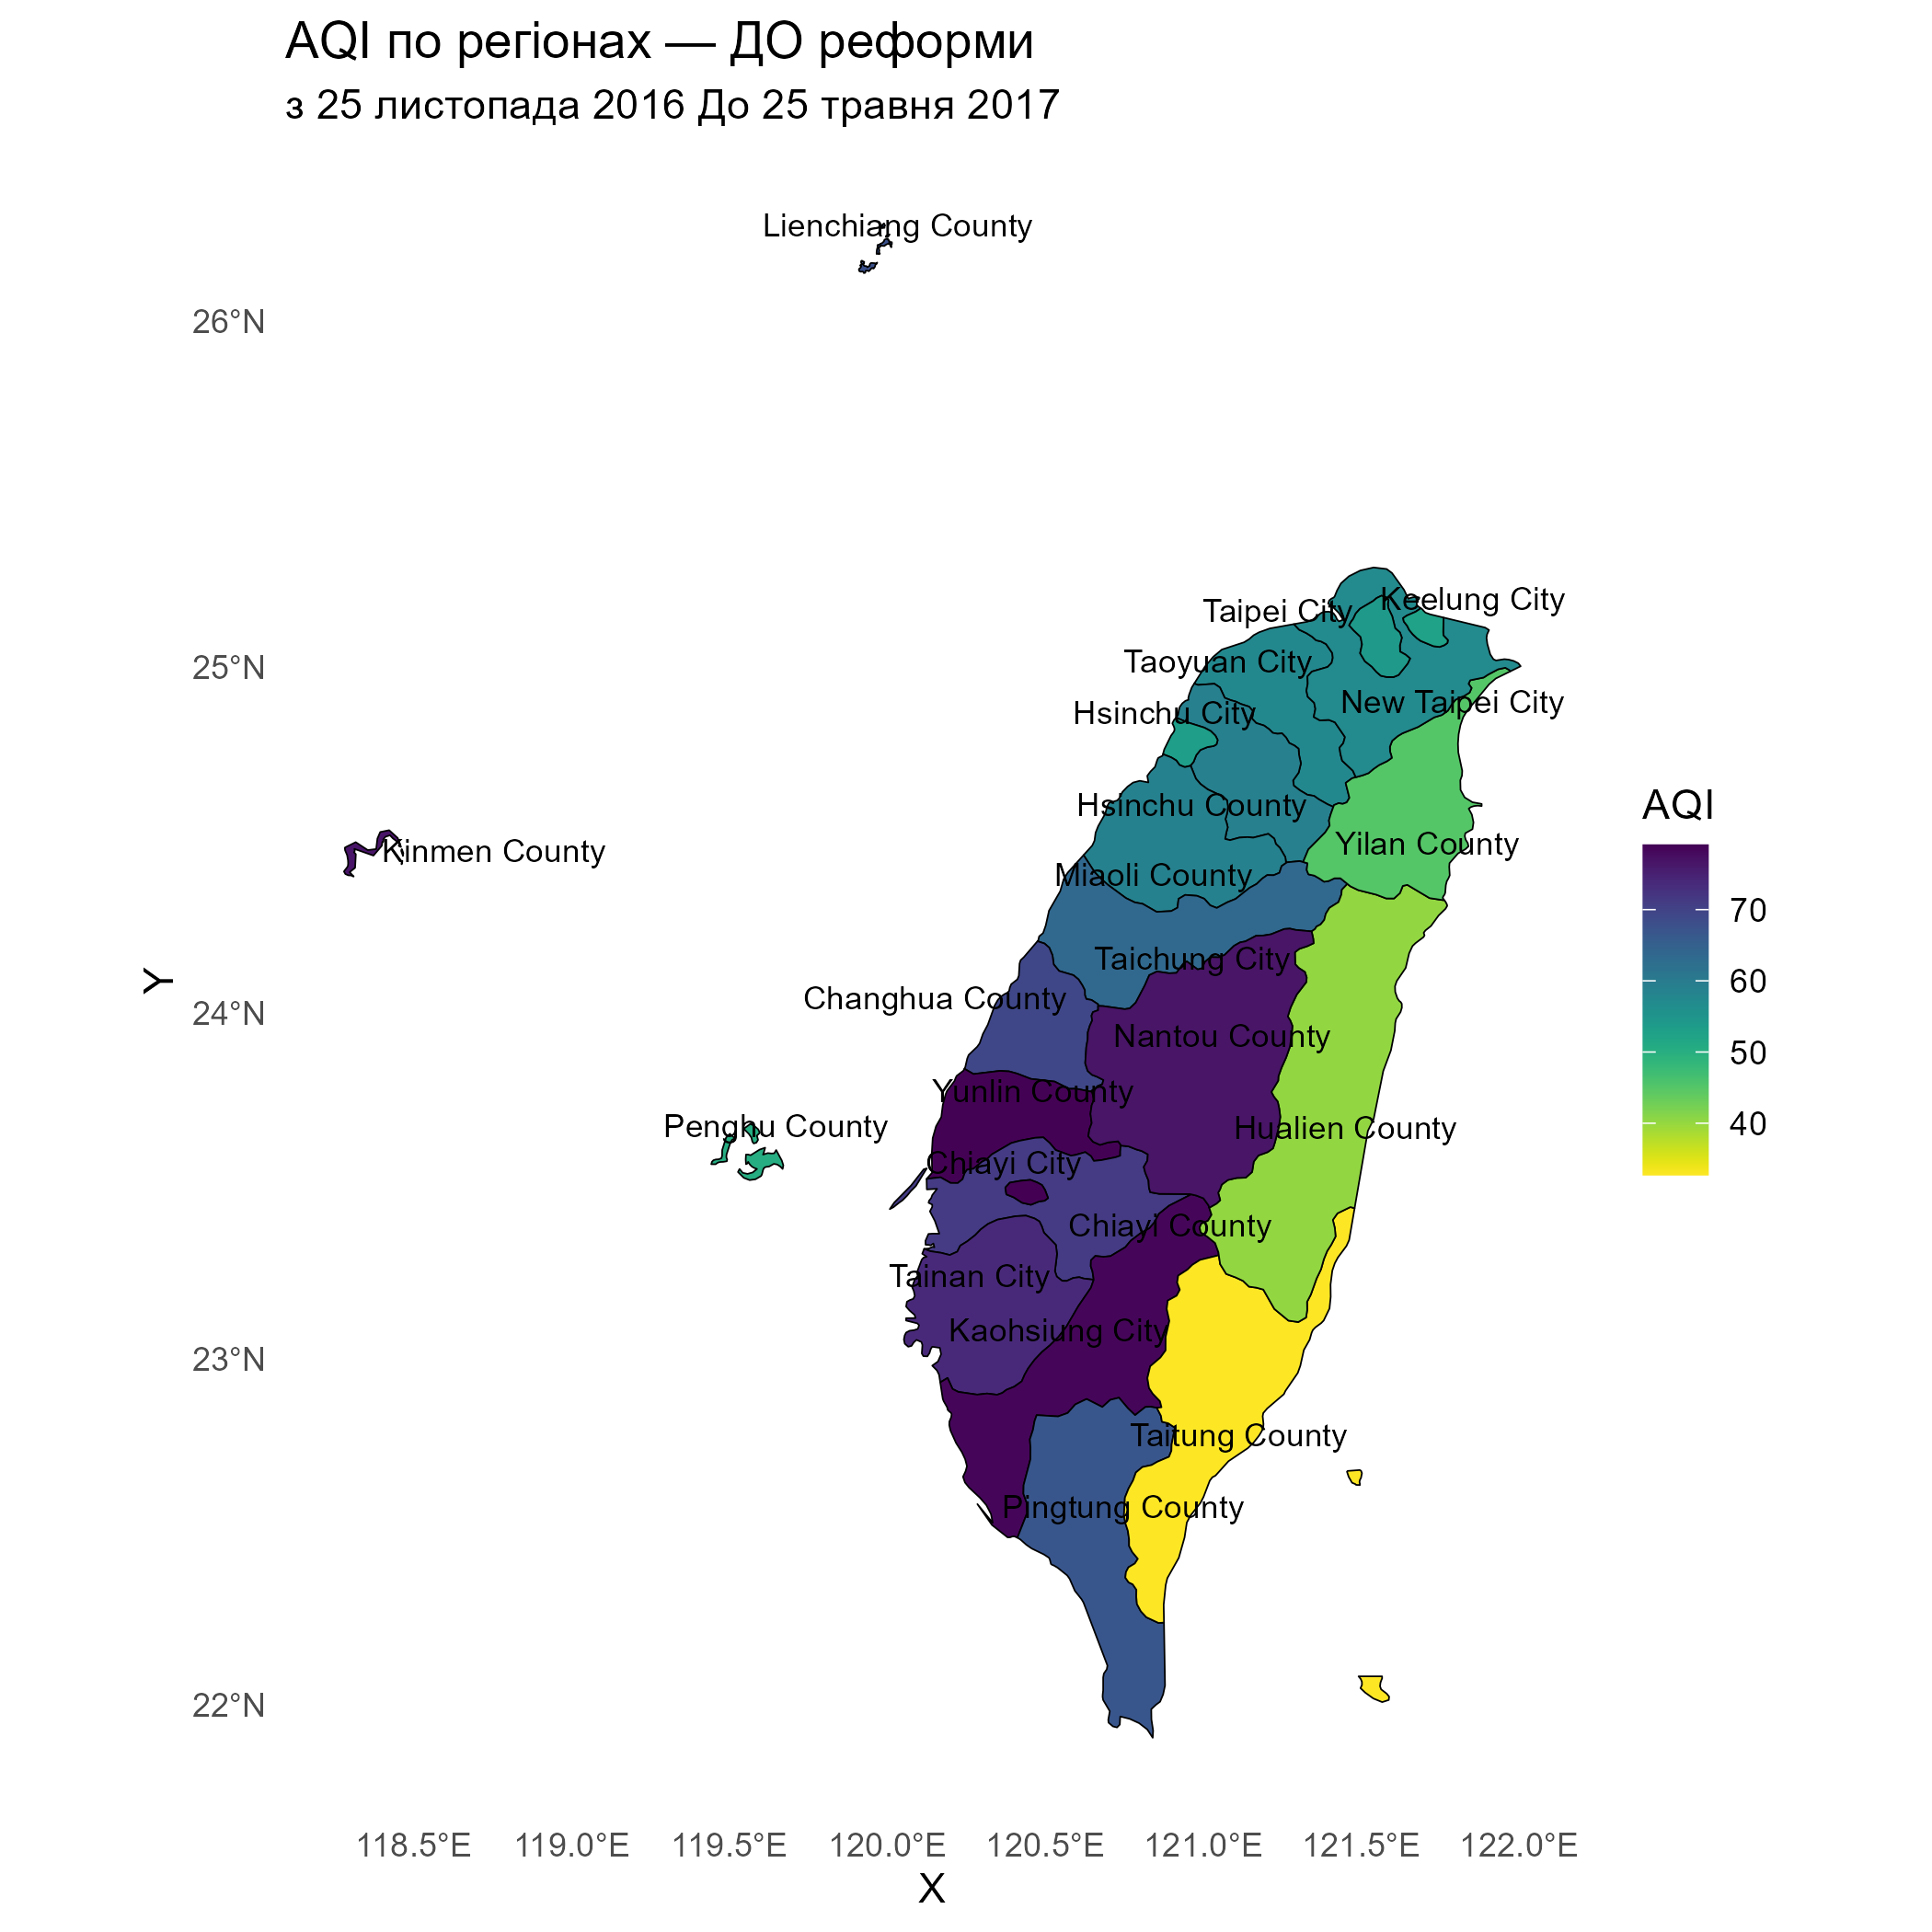
\includegraphics[width=6in]{plots/question5/map_before_reform.png}
    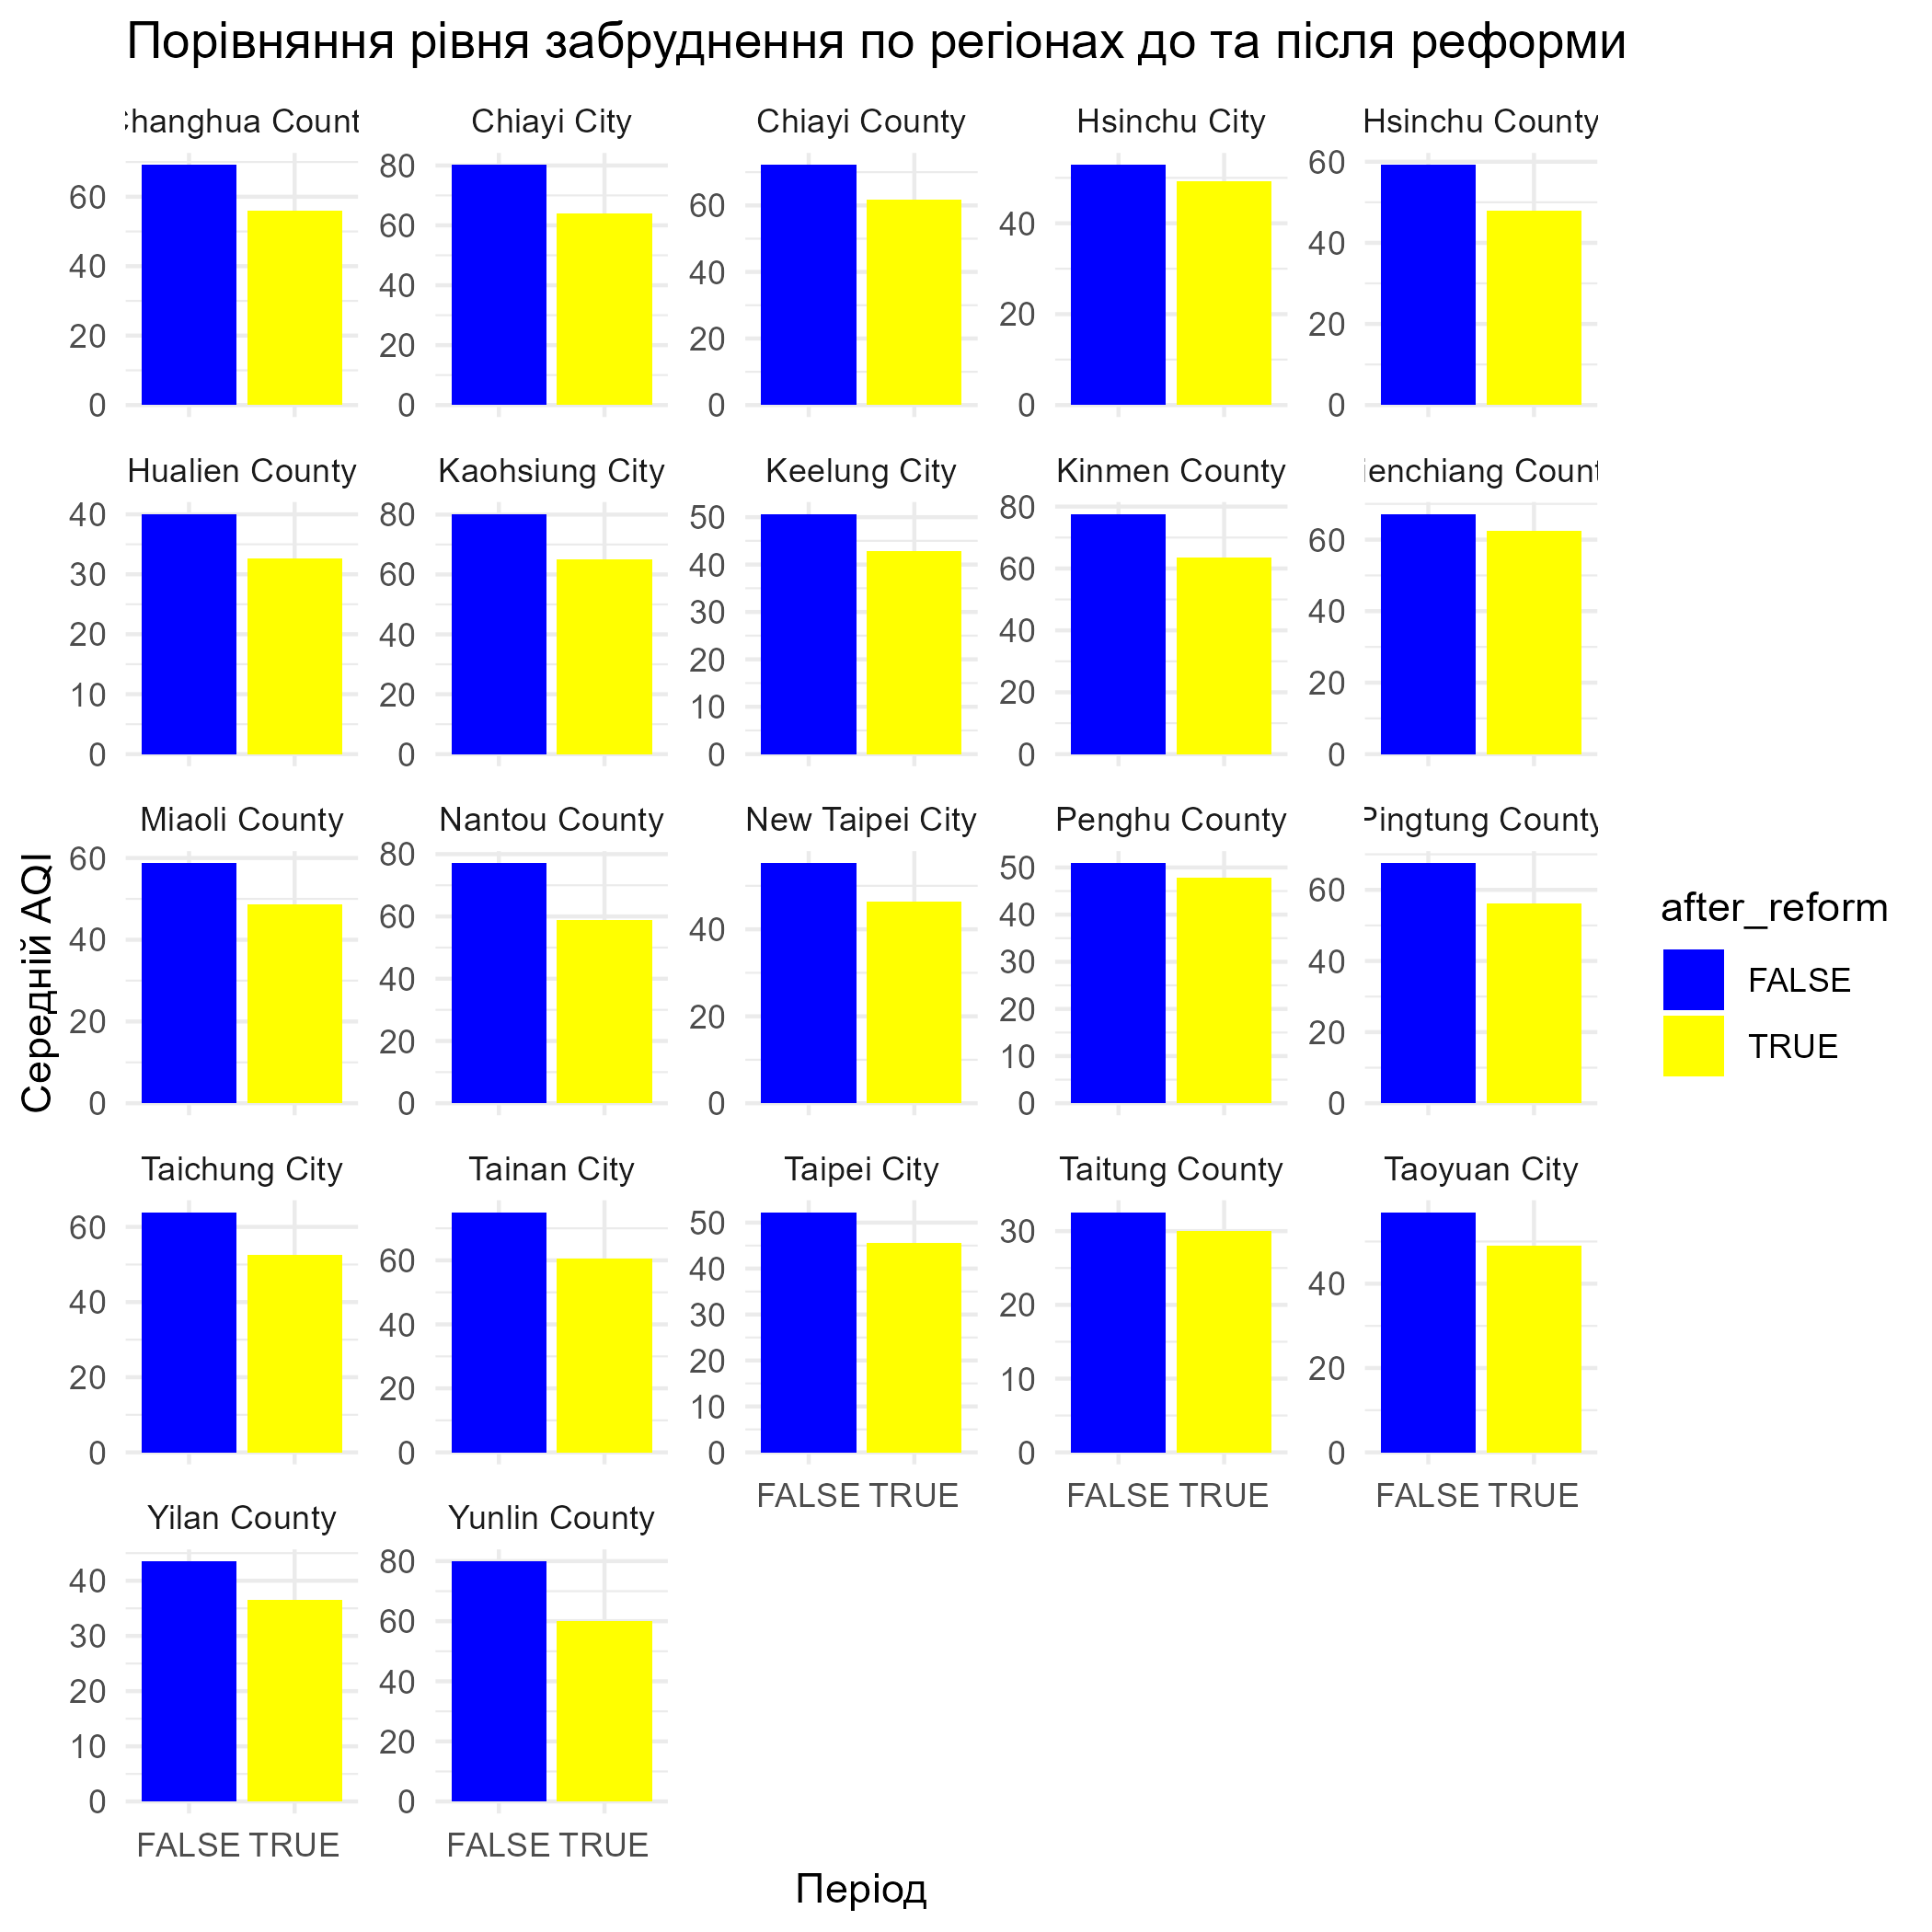
\includegraphics[width=6in]{plots/question5/region_comparison_aqi.png}
    \end{center}

    Отже, можна однозначно сказати, що загальний рівень якости повітря по регіонам покращується після реформи, це можна відмітити по насиченості забарвлення регіонів. 
    Також варто відмітити не рівномірний розподіл (зафарбовування). Провівши дослідження по таким питаняням як кількість населення та промислові регіони, було виявлено наступне: 
    \begin{figure}
        \centering
        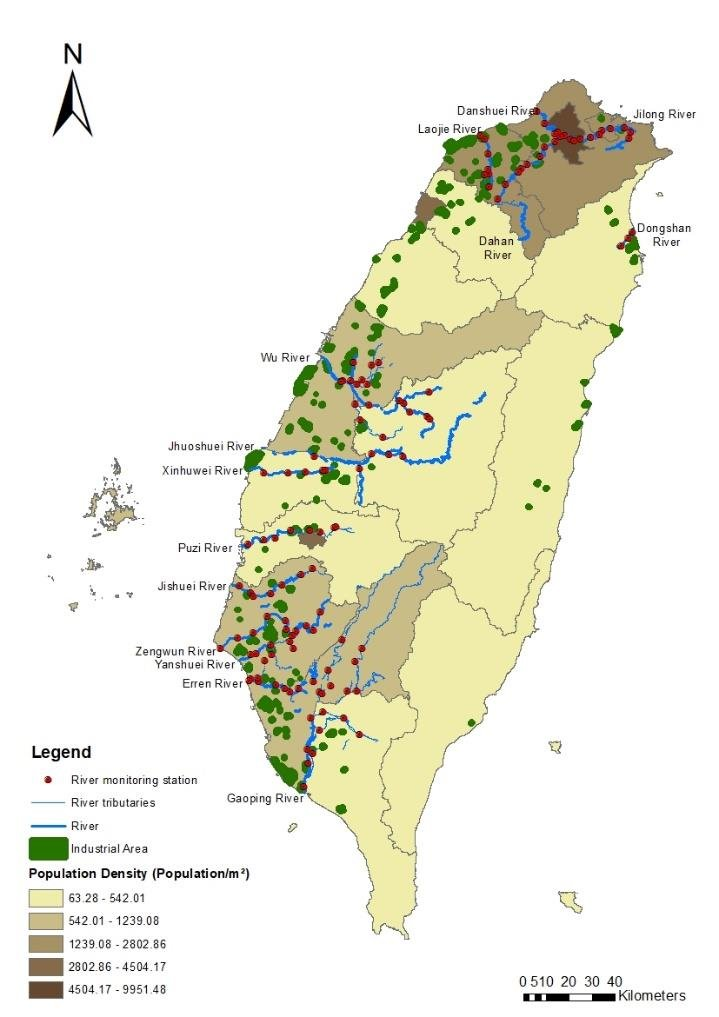
\includegraphics[width=6in]{notes/media/Study-area-of-Taiwan-representative-rivers-population-density-and-industrial-area-map.png}
        \caption{Мапа розміщення промислових зон та кількості населення по регіонам}
        \label{fig:map_after_reform}
    \end{figure}
    \footnote{\href{https://www.researchgate.net/figure/Study-area-of-Taiwan-representative-rivers-population-density-and-industrial-area-map_fig1_327245998}{Покликання на ресурс з мапою та дослідженням}}
    

    \begin{itemize}
        \item На мапі, що ми отримали, темними кольорами зафарбовані промислові та густо населені регіони. 
        Отже це може бути одним з факторів погіршення якости повітря загалом у республіці.
        \item
            \begin{quote}
            До найбільш серйозних екологічних проблем відносяться забруднення повітря, забруднення води промисловими водами та каналізацією, 
            зараження джерел питної води, незаконне вивезення тварин, занесених до Червоної книги, а також
            забруднення радіоактивними відходами. Загрозу здоров'ю населення і місцевих лісах становлять кислотні дощі. 
            На думку місцевих вчених, понад половина кислотних опадів потрапляє на острів з материкової частини Китаю під час періоду мусонів.
            \end{quote}
            \href{https://uk.wikipedia.org/wiki/%D0%A2%D0%B0%D0%B9%D0%B2%D0%B0%D0%BD%D1%8C_(%D0%BE%D1%81%D1%82%D1%80%D1%96%D0%B2)}{Покликання на статтю у Вікіпедії}
            
            Тобто саме з південних регіони найближче до материкової частини Китаю, тому "страждають" від природних катаклізмів.
        
    \end{itemize} 

    \item Чи існує залежність між початком реформ та показниками забруднення?
    
    \quad \textit{Був використаний tidy набір даних}

    \begin{center}
    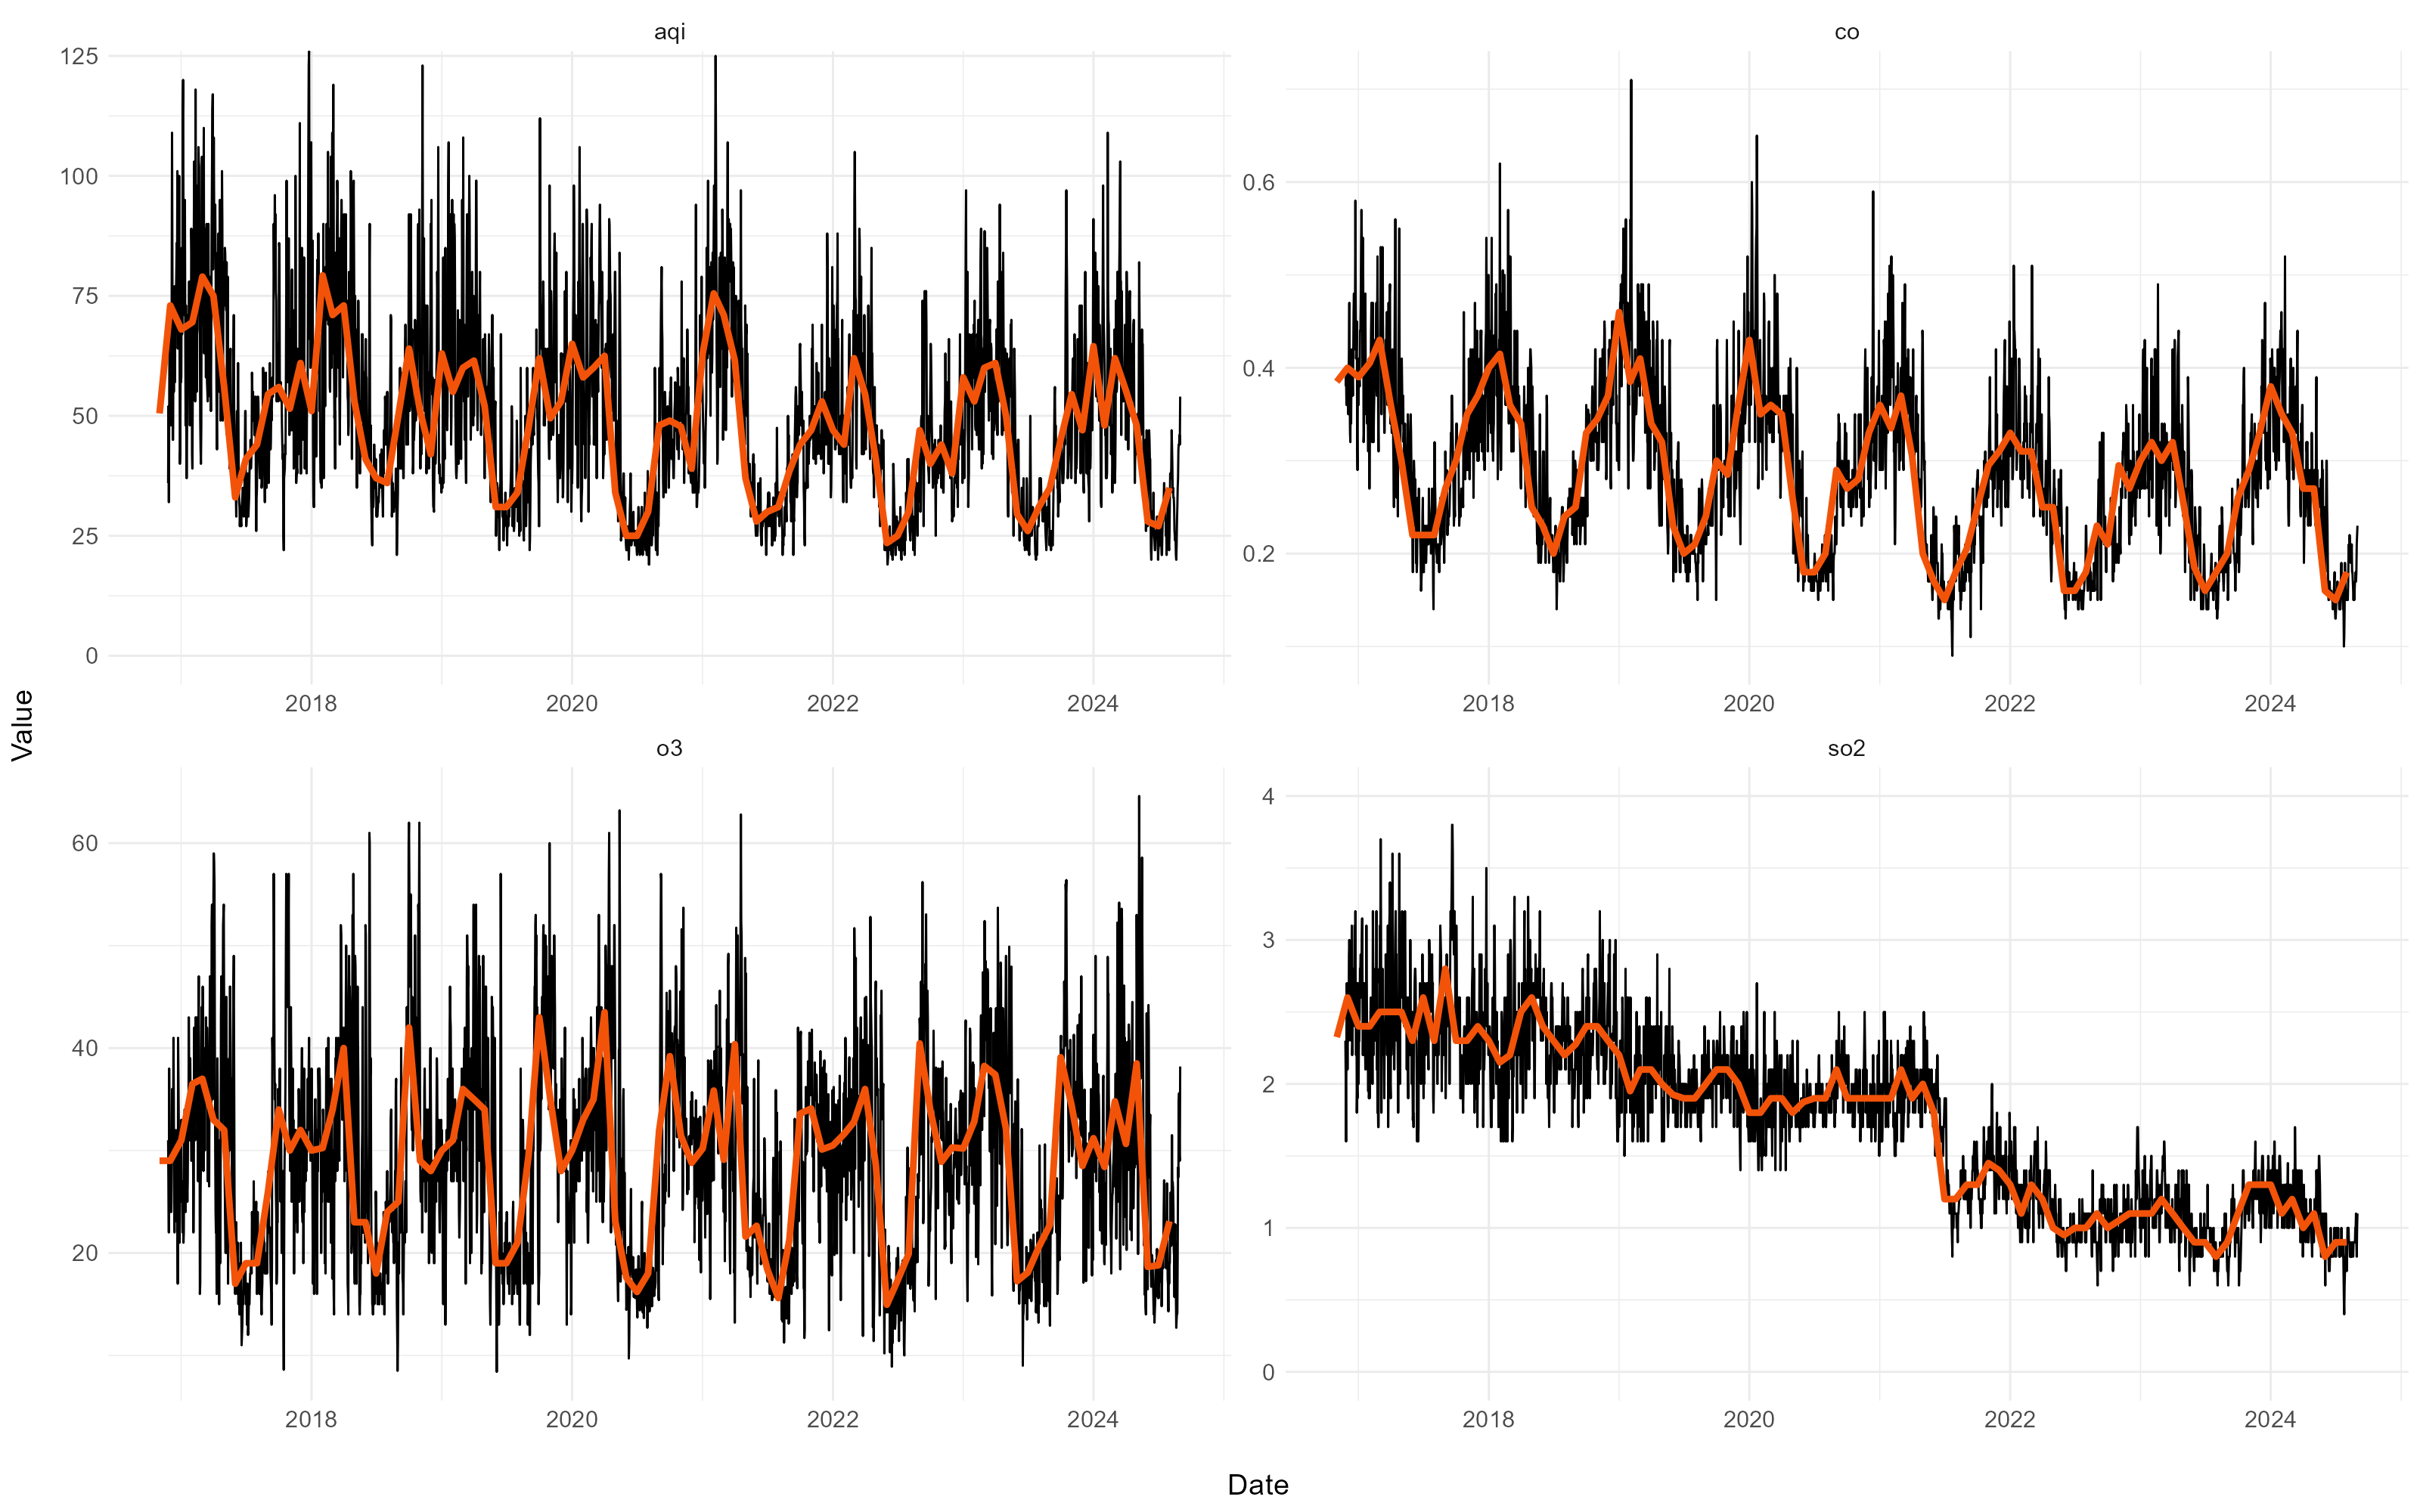
\includegraphics[width=6in]{plots/question6/line-p1.png}
    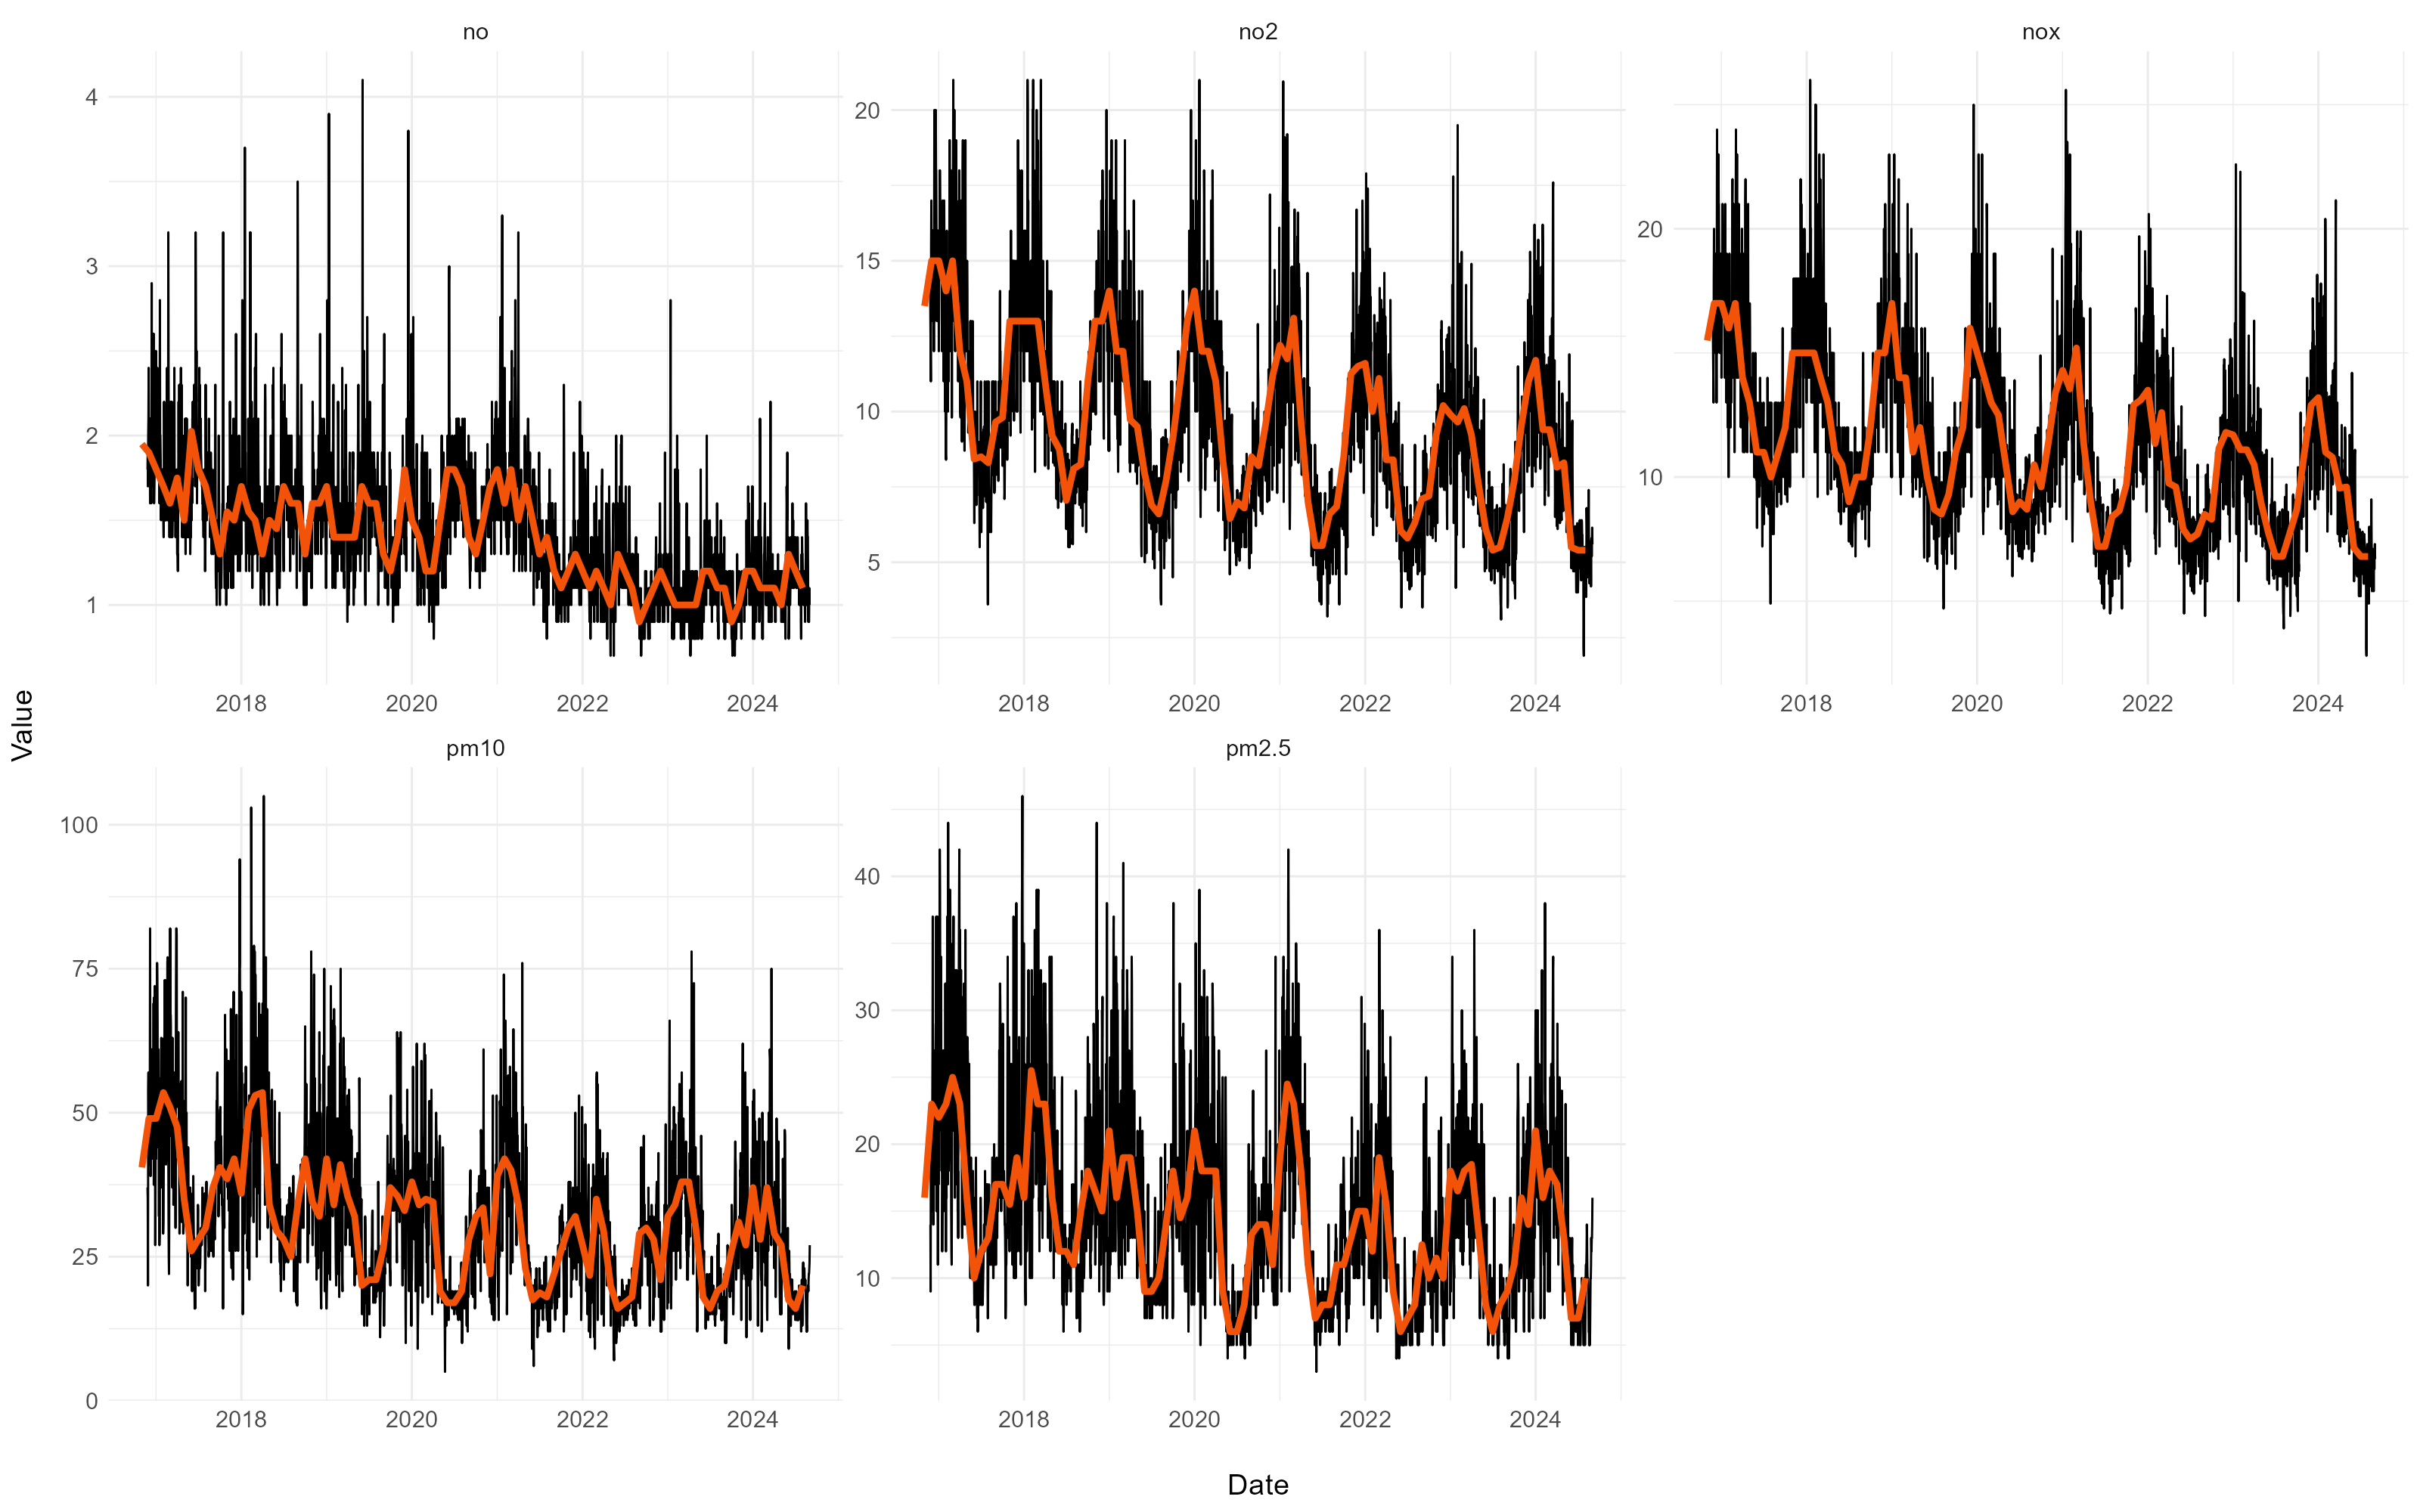
\includegraphics[width=6in]{plots/question6/line-p2.png}
    \end{center}

    Аналізуючи діаграму розсіювання для кожного типу забруднювача можна сказати, що помітні зміни і залежність від реформи зявилась лише у $SO_2$. Також не значне покращення є у $NO$.
    Всі інші показники відносно без змін. Чим це може бути обгрунтовано? Можливо зменшили викиди певні промислові регіони.
    
    \item Як змінюється якість повітря залежно від станції виміру у містах?
    
    \quad \textit{Був використаний trimmed набір даних}

    \begin{center}
    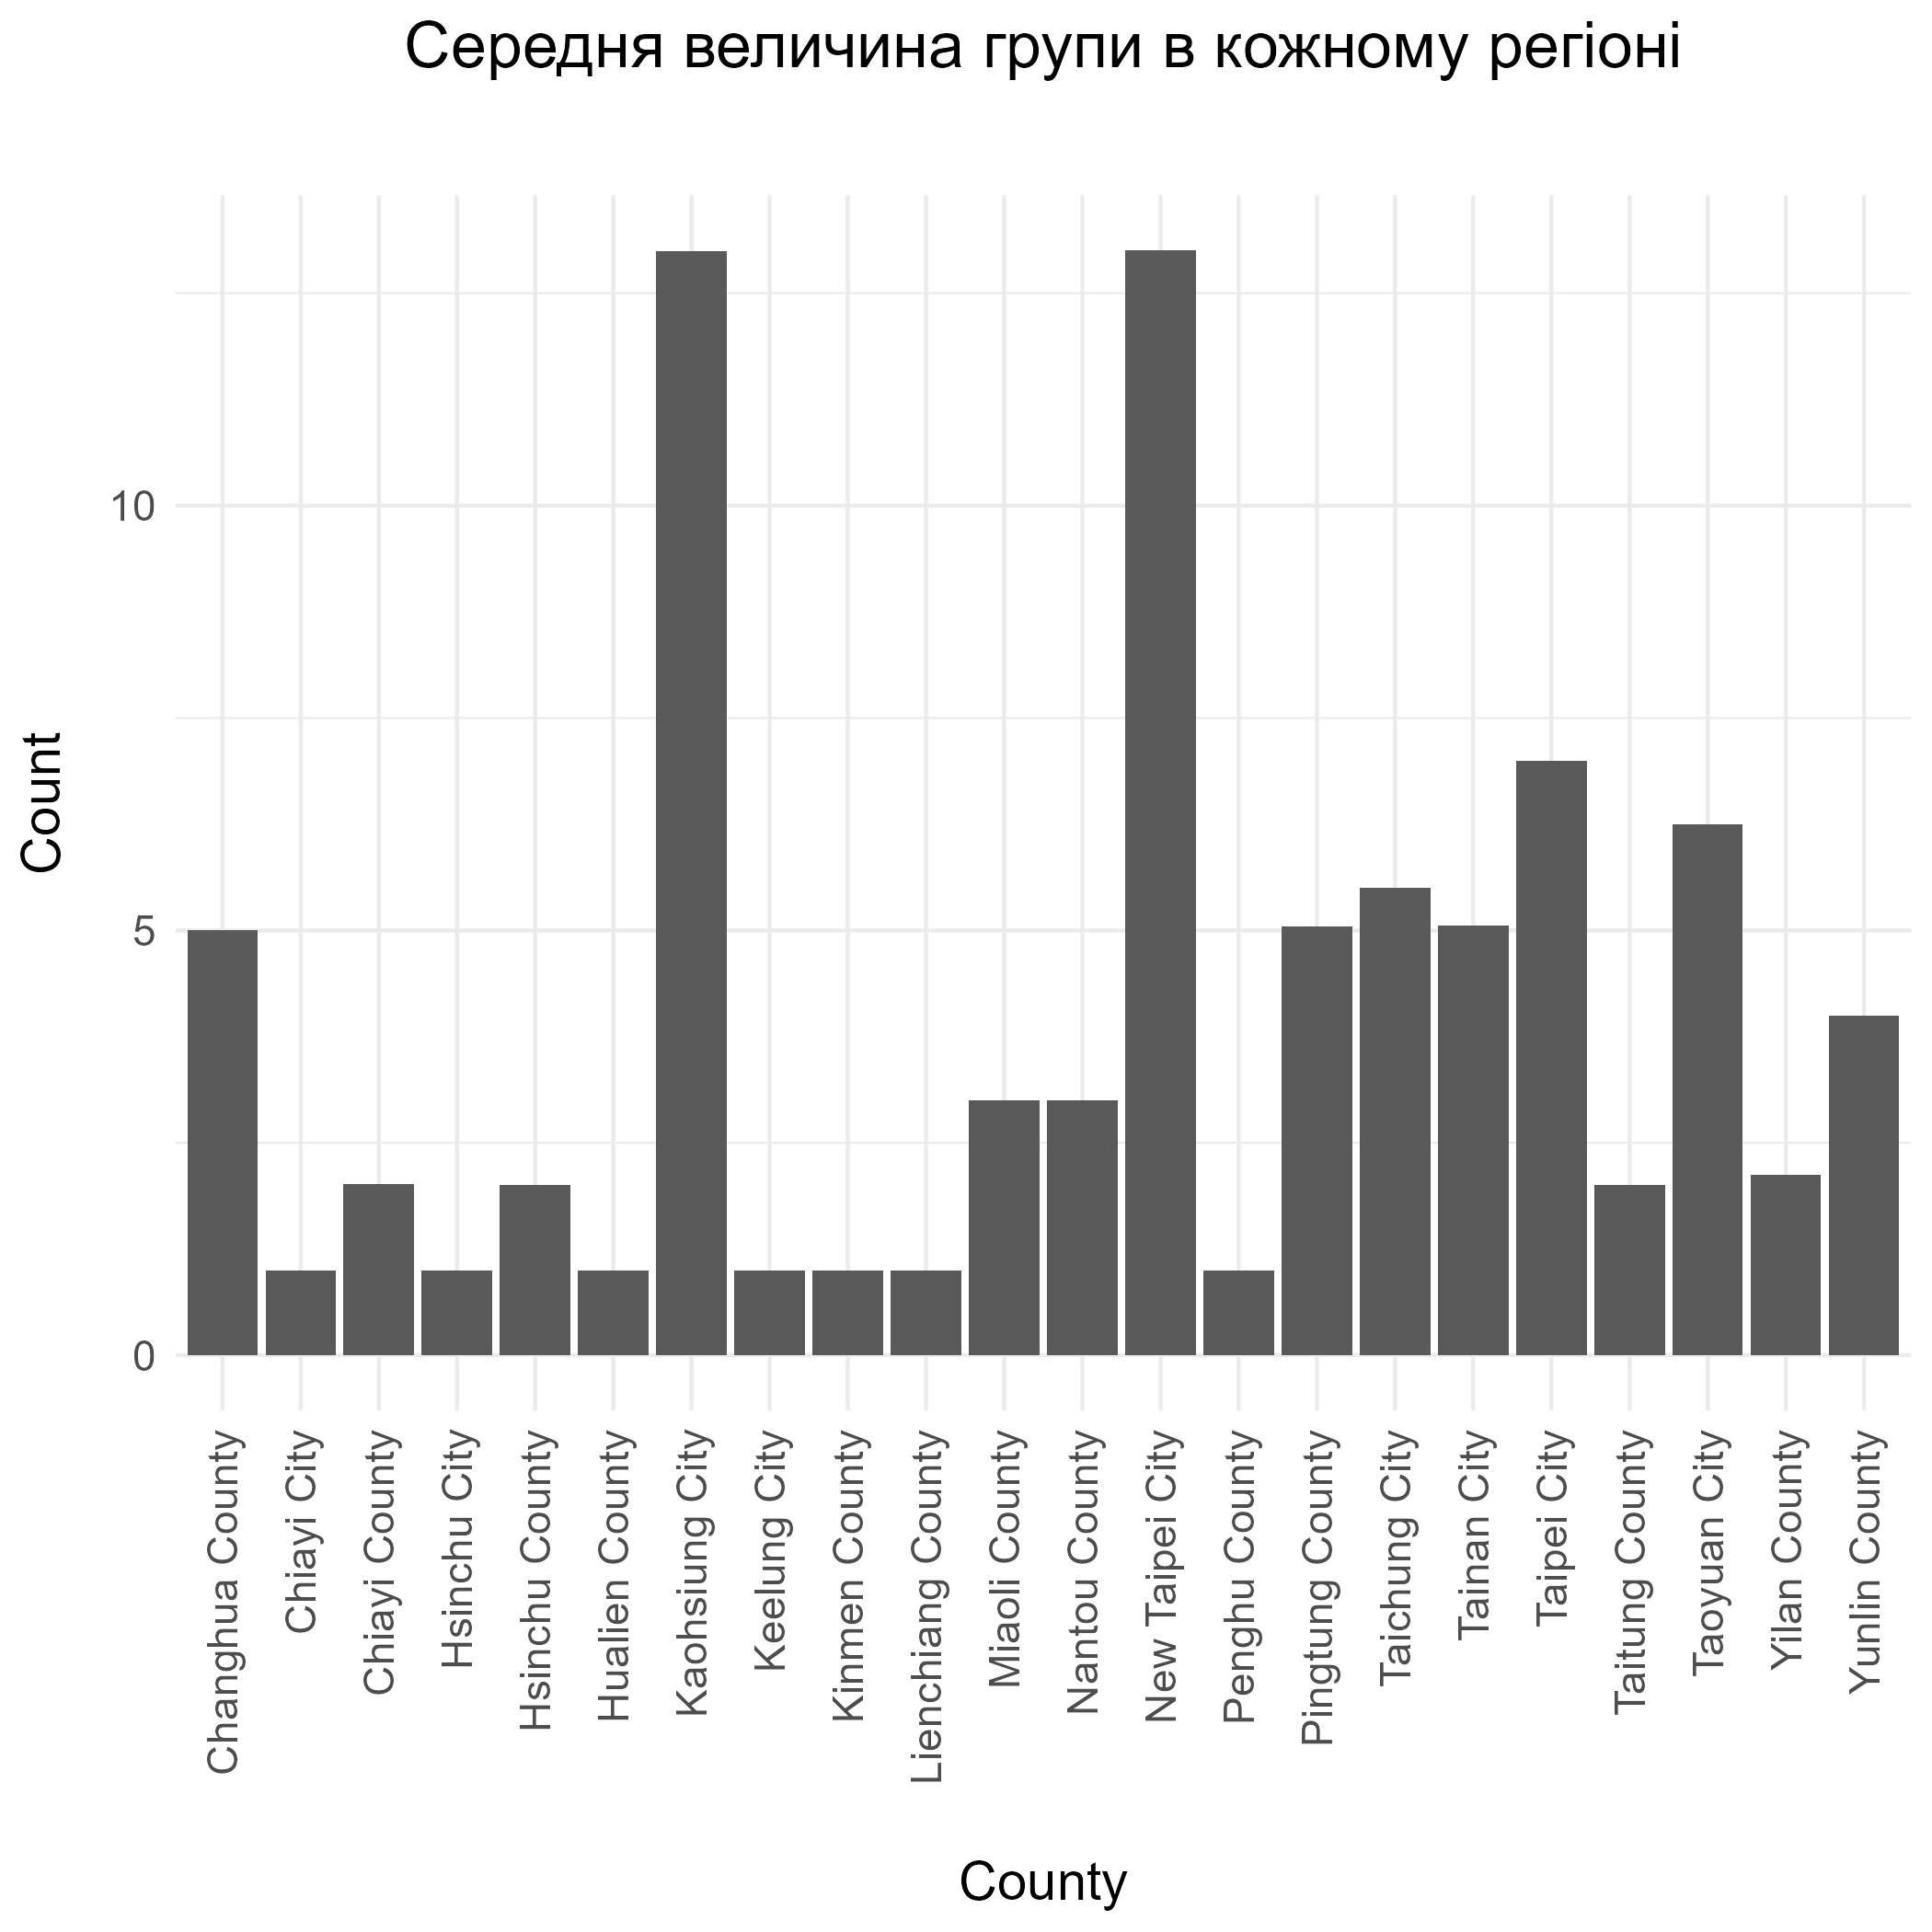
\includegraphics[width=6in]{plots/question7/bar-count.png}
    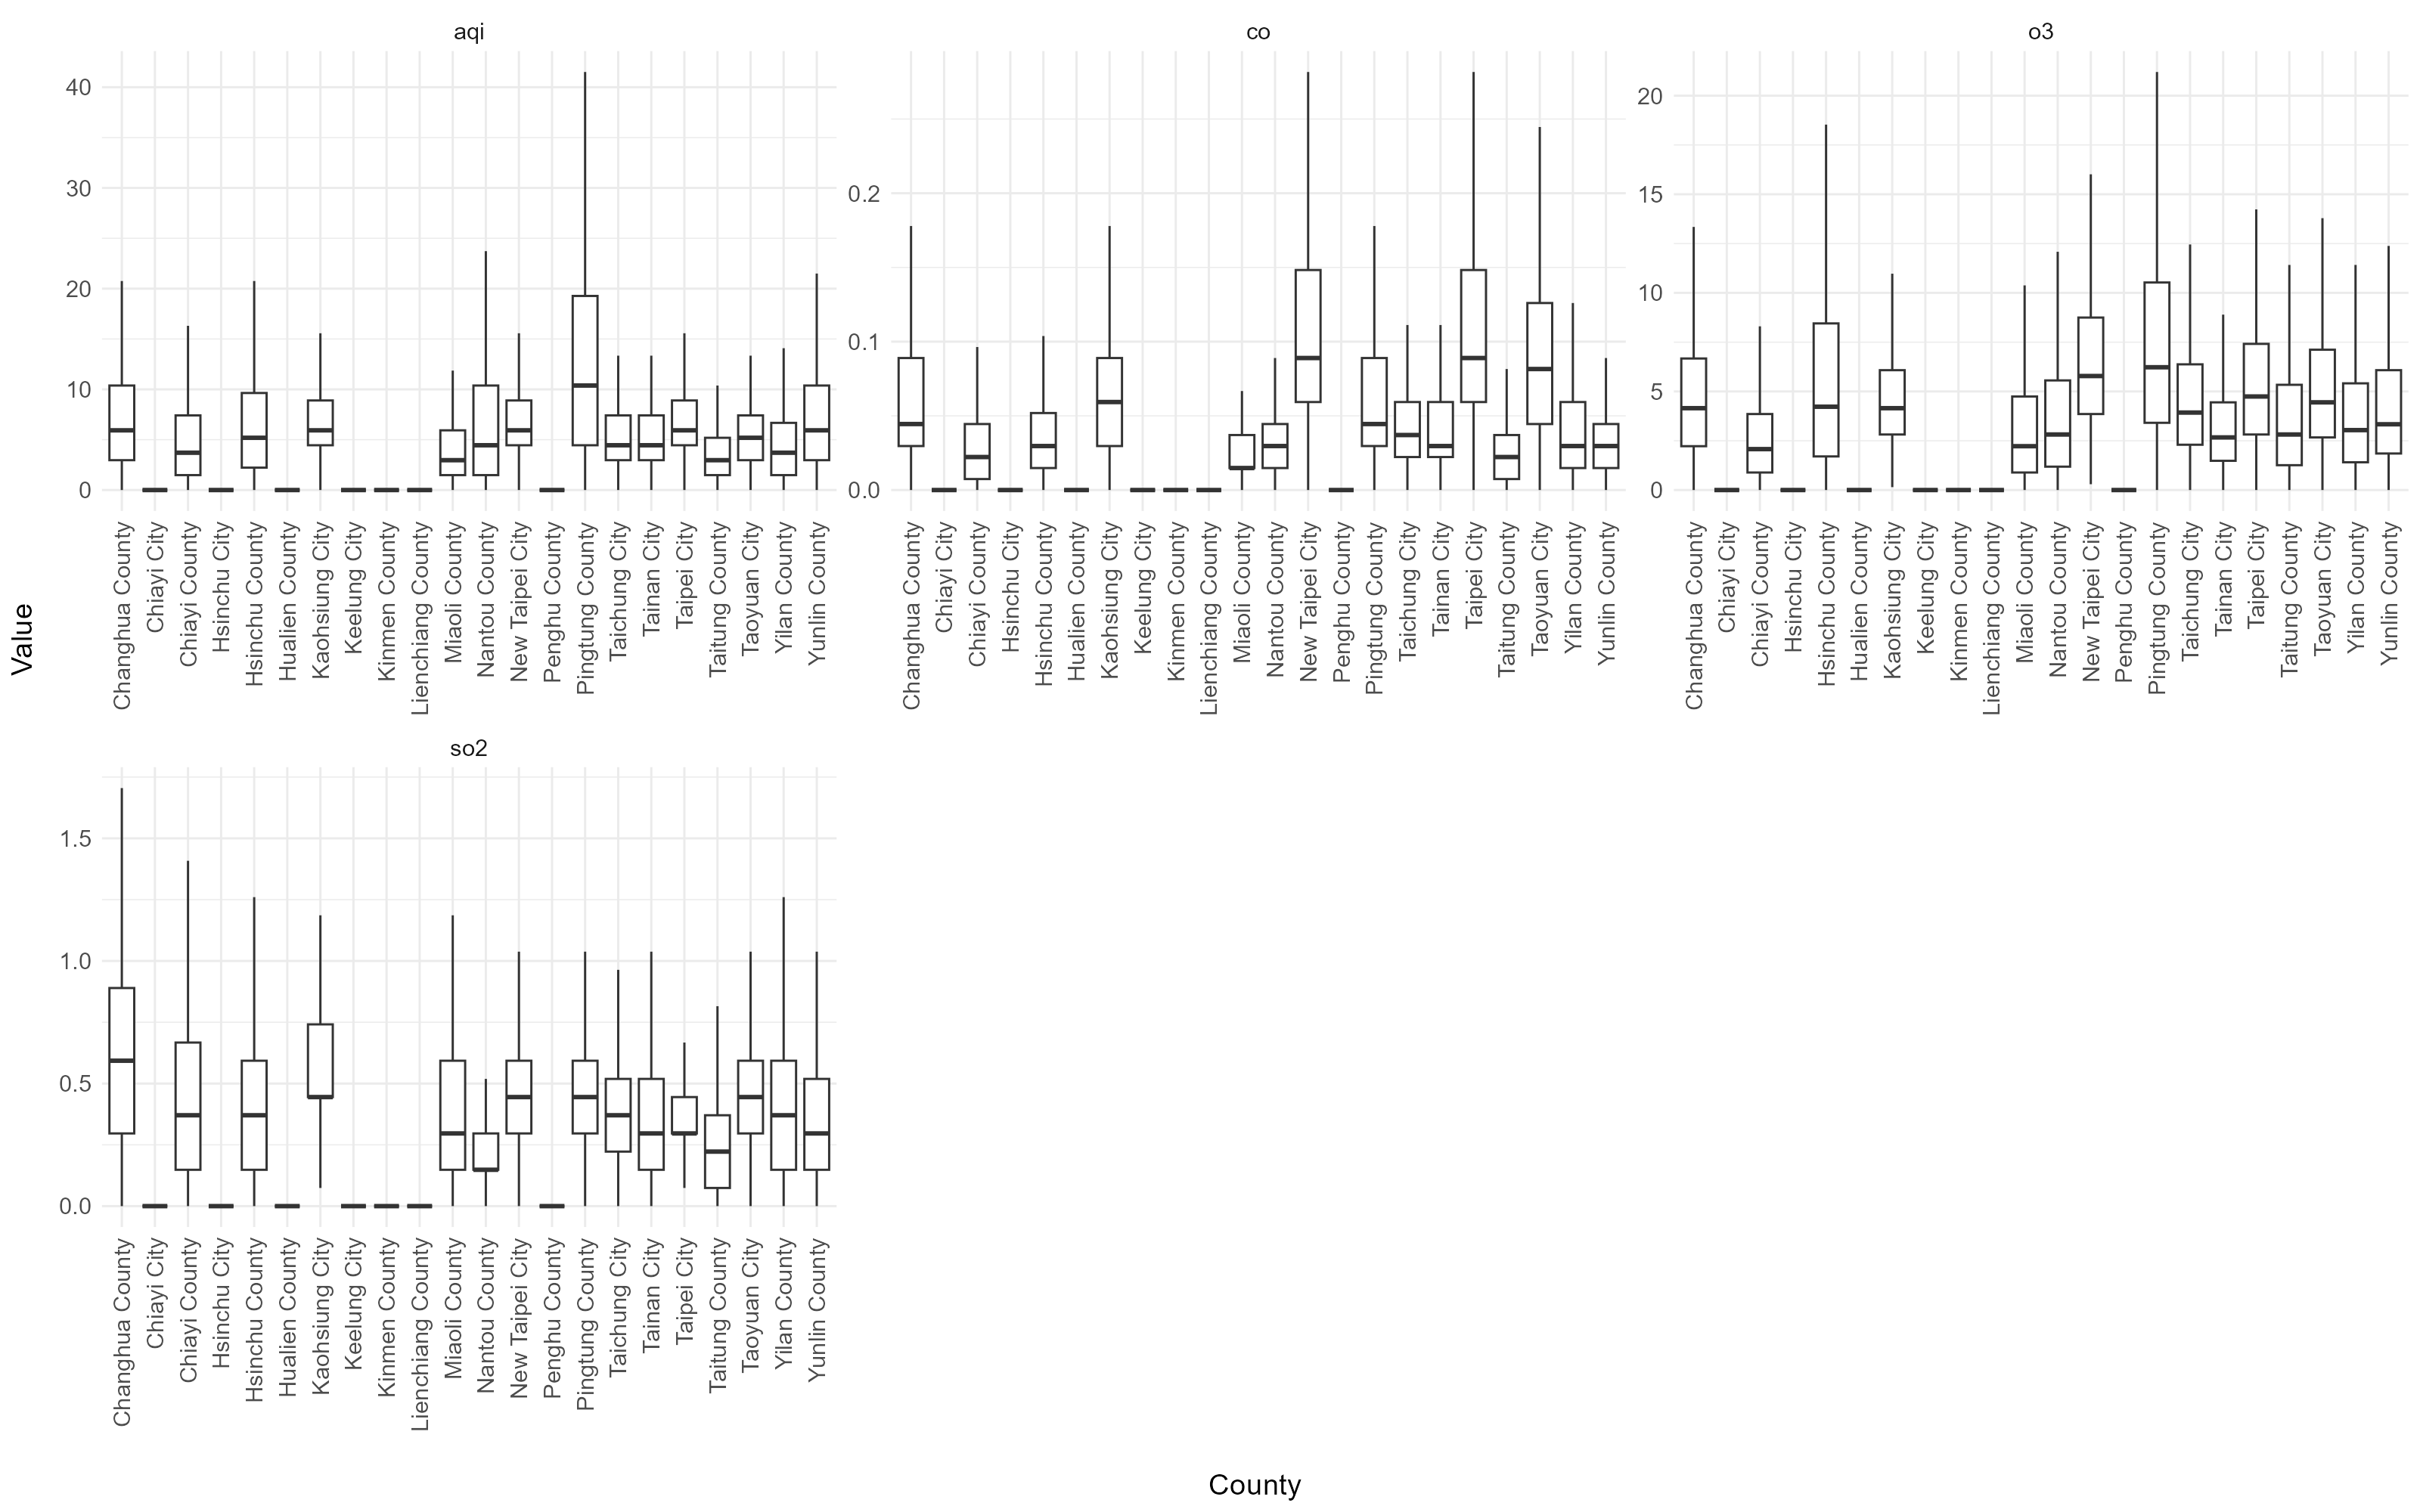
\includegraphics[width=6in]{plots/question7/box-county-p1.png}
    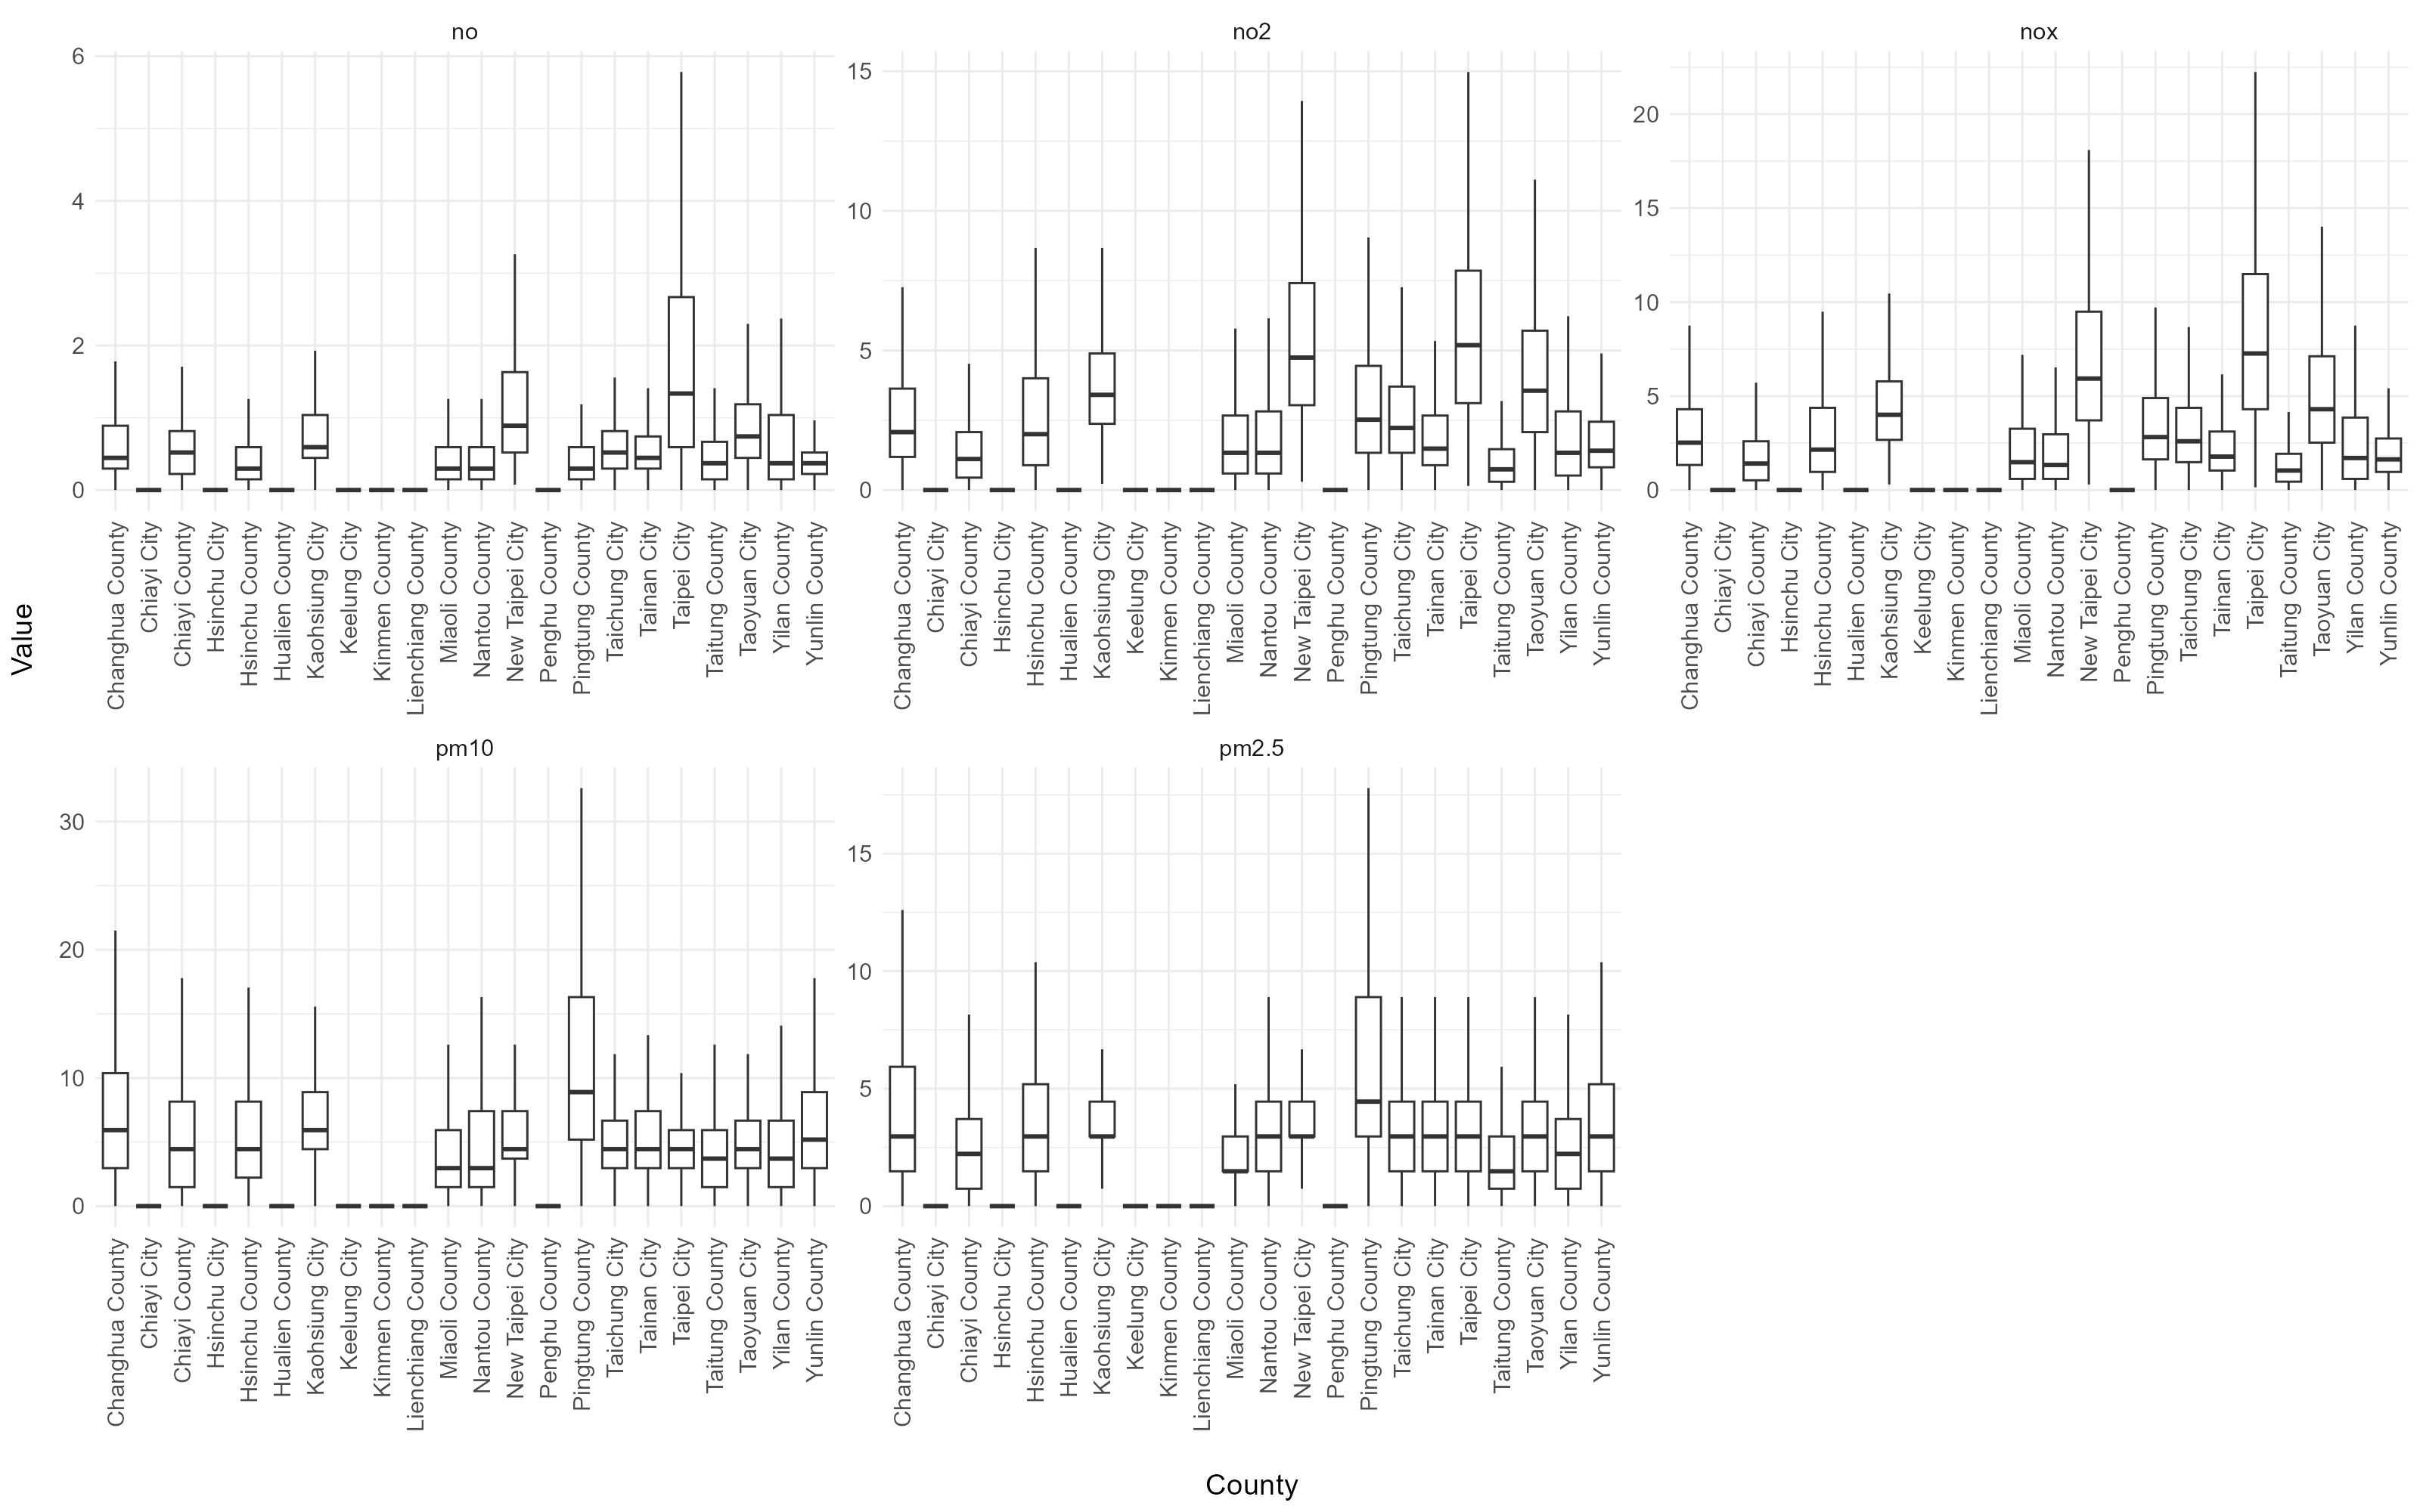
\includegraphics[width=6in]{plots/question7/box-county-p2.png}
    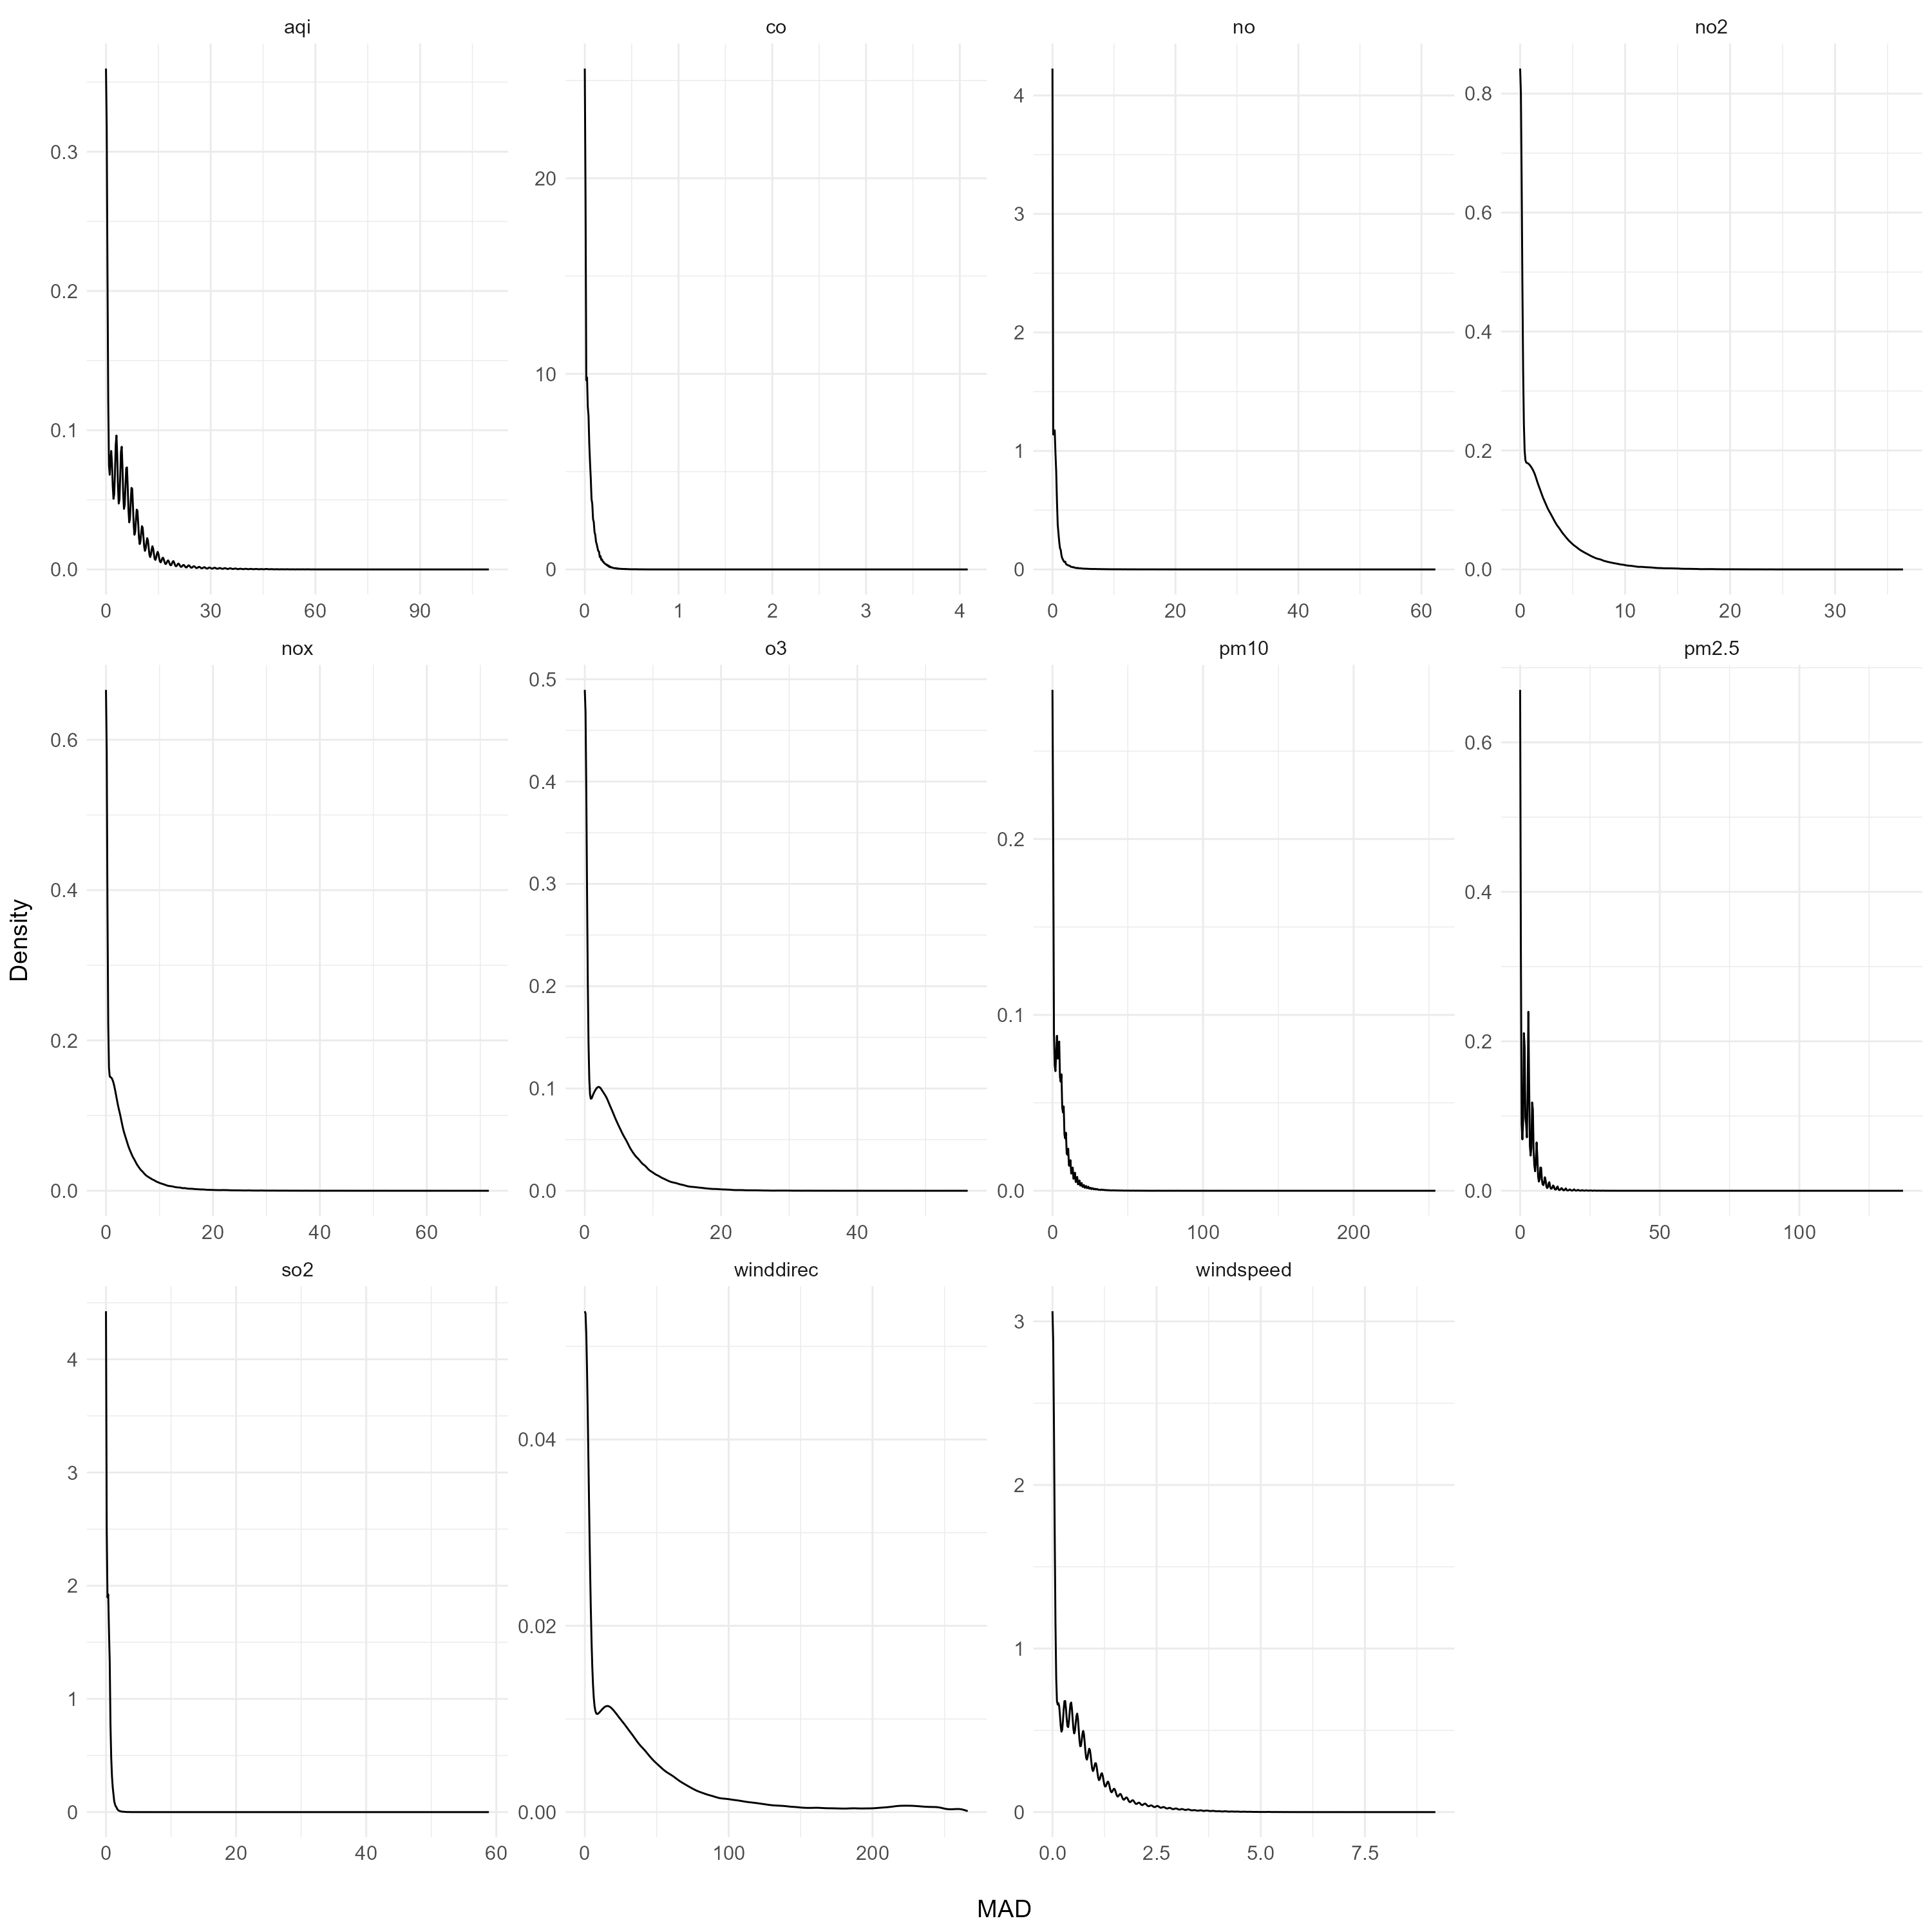
\includegraphics[width=6in]{plots/question7/density.png}
    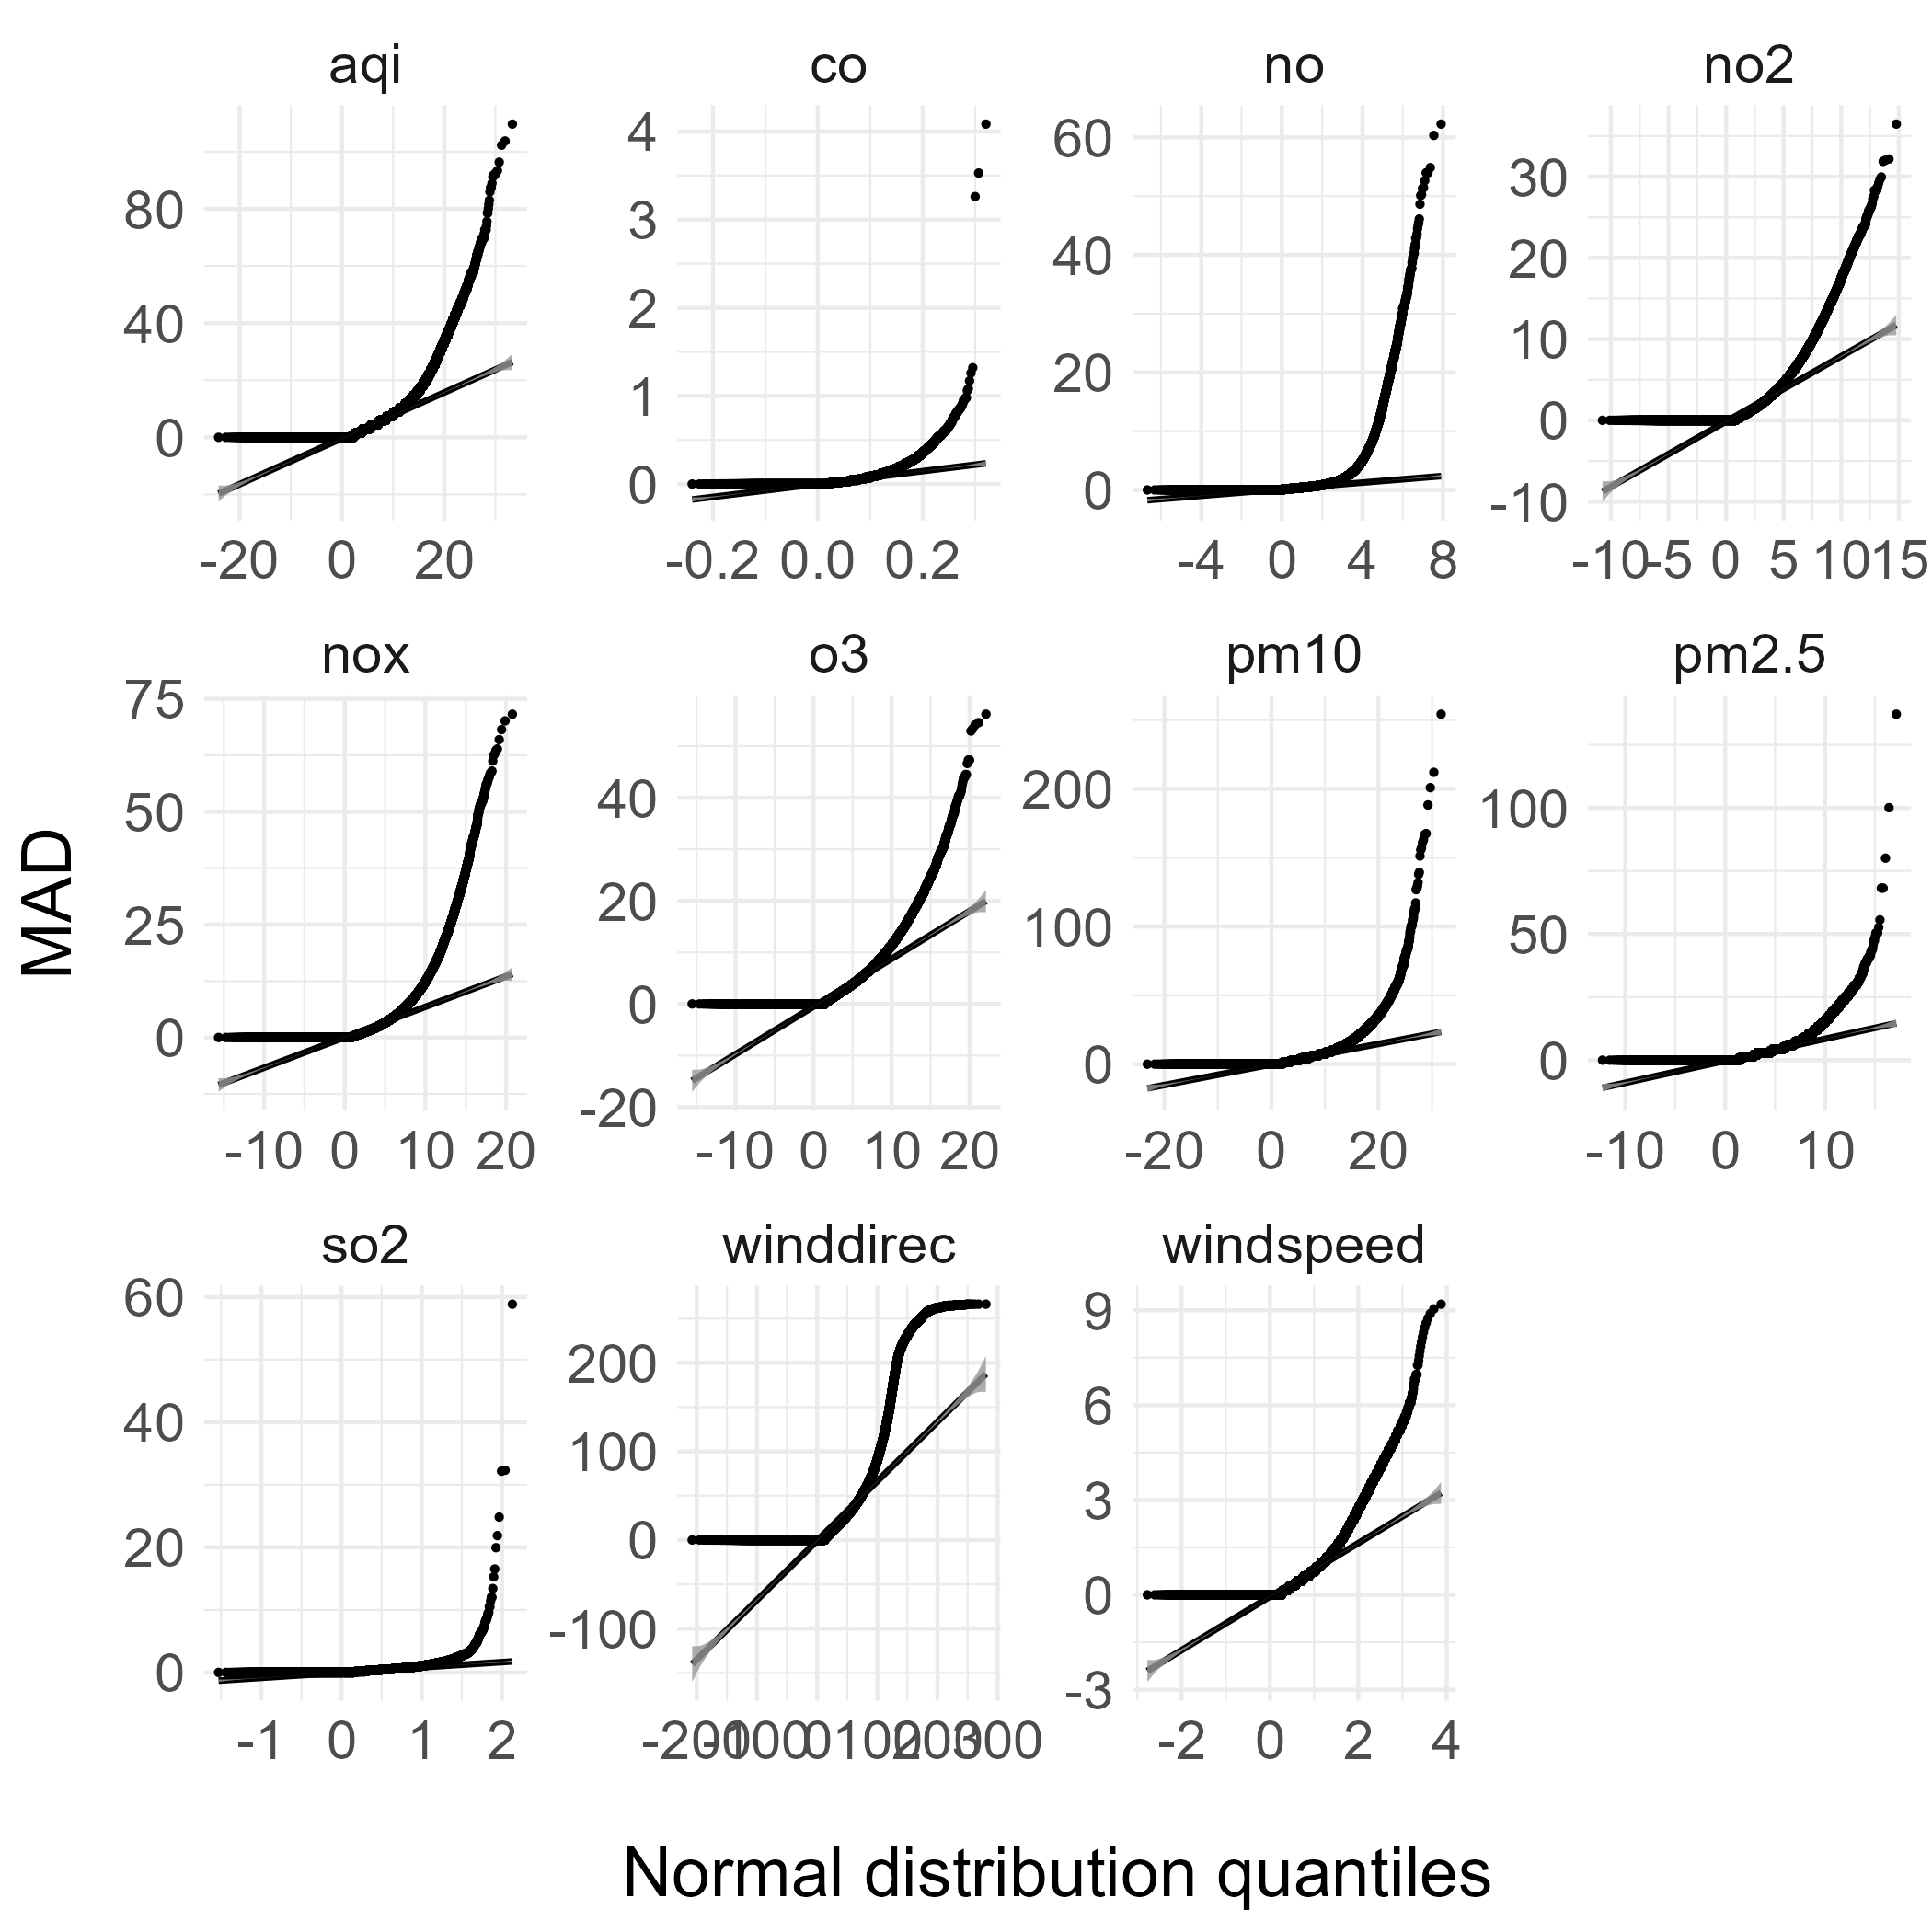
\includegraphics[width=6in]{plots/question7/qq.png}
    \end{center}
    Найбільший MAD у `winddirec`. Це можна пояснити природною різницею напрямку вітру залежно від місця знахоження.

    На графіку видно, що зміна показників не є рівномірно розподілена по регіонам. В загальному можна зробити висновок, що для більшості 
показників зміна значення залежно від станції вимірювання не є суттєвою.
\end{enumerate}

\pagebreak

\newpage
\section{ВИСНОВОК}
Питання якости повітря в світі зараз досить акутальне, тому було стандартизовано деякі показники, які дозволяють розуміти стан повітря.
Нижче наведена загальна таблиця, яка показує шкалу та рекомендації по AQI.
\begin{table}
    \centering
    \renewcommand{\arraystretch}{1.3}
    \setlength{\arrayrulewidth}{1pt}
    \begin{tabular}{|c|c|p{8cm}|}
        \hline
        \rowcolor{gray!20} \textbf{AQI} & \textbf{Рівень якості повітря} & \textbf{Рекомендації} \\
        \hline
        \rowcolor{green!40} 0-50 & Добрий & Якість повітря відмінна. Можна безпечно перебувати на вулиці. Ідеально для занять спортом. \\
        \hline
        \rowcolor{yellow!40} 51-100 & Помірний & Прийнятна якість повітря. Чутливим групам слід обмежити тривалі прогулянки. Можливі незначні проблеми для алергіків. \\
        \hline
        \rowcolor{orange!60} 101-150 & Шкідливий для чутливих груп & Люди з респіраторними захворюваннями повинні обмежити перебування надворі. Дітям та літнім людям рекомендується залишатися вдома. Уникати активного спорту на відкритому повітрі. \\
        \hline
        \rowcolor{red!60} 151-200 & Шкідливий & Всім рекомендується обмежити перебування надворі. Використовувати захисні маски при виході. Зачиняти вікна в приміщеннях. \\
        \hline
        \rowcolor{purple!50} 201-300 & Дуже шкідливий & Серйозна загроза для здоров’я. Максимально обмежити вихід на вулицю. Використовувати очищувачі повітря в приміщеннях. \\
        \hline
        \rowcolor{black!40} 301+ & Небезпечний & Надзвичайна ситуація. Виходити тільки в разі крайньої необхідності. Обов’язкове використання респіраторів. \\
        \hline
    \end{tabular}
    \caption{Шкала оцінювання AQI та рекомендації}
    \label{tab:AQI_scale}
\end{table}
Тобто розуміючи загальні характеристики та стандарти, ми можемо зробити висновок по Тайваню.\footnote{\href{https://center-ltd.com.ua/novyny/normy-indeksu-yakosti-povitrya-yak-rozumity-pokaznyky-ta-zahystyty-svoye-zdorov-ya/}{Покликання на статтю про характеристику AQI}}

В результаті виконання лабораторної роботи було проведено розвідковий
аналіз результатів виміру якости повітря у регіонах Тайваню з 2016 року по 2024. 

На жаль не вдалось відповісти на деякі поставлені питання, 
через значну кількість відсутніх даних у стовпці $'pollutant'$, а саме не дали відповідь на: 
\begin{enumerate}
    
    \item  Чи існує кореляція між рівнем забруднення повітря (AQI) і типом головного забруднювача (pollutant) в різних районах?
    
\end{enumerate}
Відповіді на ці питання сподіваємось уряд Тайваню, зможе в скорому часі оприлюднити, 
тому що зараз можна лише припускати, що саме впливає на такий рівень забруднення.

Гістограми, побудовані на основі видобутих даних, демонструють характерну залежність тих чи інших речовин 
у повітрі відповідно до регіону, часу доби, швидкості вітру та іншого.

Отже, після розвідкового аналізу та побудови графіків, можна дати відповіді на наступні питання:
\begin{enumerate}
    \item Чи впливає швидкість вітру (windspeed) на концентрацію частинок PM2.5 і PM10?
    
    Ні, на жаль, швидкість вітру має не значний вплив на концентрацію цих частинок, так як це тверді речовини. 
    
    \item Як зміни в концентрації  $O_3$  та $SO_2$ впливають на загальний рівень забруднення повітря (AQI)?
    
    Концентрація $O_3$ має більший вплив на загальний рівень AQI ніж $SO_2$.

    \item Як змінюється якість повітря (status) протягом доби в різних районах?
    
    Протягом доби якість повітря не зазнає значних змін. В загальному є незначне покращення пообіді. 

    \item Які регіони (county) мають найвищий середній рівень забруднення повітря (AQI) протягом року?
     
    Найвищий середній рівень забруднення повітря (AQI) протягом року мають такі регіони: 
    \begin{itemize}
        \item Kinmen County	 
        \item Lienchiang County
        \item Chiayi County	 
        \item Chiayi City	     
        \item Yunlin County	 
        \item Kaohsiung City	 
        \item Tainan City	     
        \item Nantou County	 
        \item Changhua County	 
        \item Taichung City	 
    \end{itemize} 

    \item Як змінився загальний рівень забруднення по регіонам після початку реформи?
    
    Загальний рівень AQI по регіонам зменшується, тобто показники покращуються після початку реформи.
    Більш явні зміни помітні через декілька років, після початку, що є цілком логічним. 
    Якщо уряд продовжить вводити обмеження та покращувати систему реформ, то показники в усій республіці нормалізуються. 

    \item Чи існує залежність між початком реформ та показниками забруднення?
    
    Після побудови низки гарфіків, було відмічено, що після реформи суттєво змінився 
    лише показник концентрації $S0_2$ та незначні зміними $NO$. Всі ініші показники, не зазнали суттєвих змін.
    
    \item Як змінюється якість повітря залежно від станції виміру у містах?
    
    Якість повітря змінюється нерівномірно у містах. Тобто саме від станції виміру не залежить, 
    на це впливають інші фактори, які зазначені вище.

\end{enumerate}


\newpage
\section{Використані джерела}
\begin{enumerate}
    \item Exploratory Data Analysis with R. Home | Bookdown. 
    
    URL:  \href{https://bookdown.org/rdpeng/exdata/}{https://bookdown.org/rdpeng/exdata/}
    
    \item Exploratory Data Analysis | R for Data Science. Welcome | R for Data Science.
    
    URL: \href{https://r4ds.had.co.nz/index.html}{https://r4ds.had.co.nz/index.html}
    \item The R Graph Gallery – Help and inspiration for R charts. The R Graph Gallery. 
    
    URL: \href{ https://r-graph-gallery.com/}{ https://r-graph-gallery.com/ }

    \item Учасники проектів Вікімедіа. Тайвань (острів) – Вікіпедія. Вікіпедія.
     
    URL: \href{https://uk.wikipedia.org/wiki/Тайвань\_(острів)}{\url{https://uk.wikipedia.org/wiki/Тайвань_(острів)}} 

    \item Air quality index (AQI)(historical data) 
    
    URL: \href{https://data.moenv.gov.tw/en/dataset/detail/aqx\_p\_488}{\url{https://data.moenv.gov.tw/en/dataset/detail/aqx_p_488}}

    \item Стаття: "План дій виконавчого врядуваня щодо контролю над забрудненням повітря. Центр екологічної інформації."
    
    URL:\href{https://e-info.org.tw/node/209138}{https://e-info.org.tw/node/209138} 

\end{enumerate}

\end{document}